\documentclass[phd,black]{PrincetonThesis}
\usepackage[margin = 1in]{geometry}
\usepackage{amsmath}
\usepackage{tikz-feynman}
\usepackage{bm}
\usepackage{fancyhdr}
\usepackage{hyperref}
\usepackage{hepnames}
\usepackage{multirow}
\usepackage{epsfig}
\usepackage{subfigure}
\usepackage{slashed}
\usepackage{amssymb}
\usepackage{array}
\usepackage{fp}
\usepackage{acronym} %texorpdfstring
\usepackage{ifthen}
\usepackage{ptdr-definitions}
\usepackage{topcapt}
\pagestyle{fancy}

\newcolumntype{T}{>{\trunc}r}
\def\trunc\ignorespaces#1\\{%
  \FPset\a{#1}
  \FPround\a\a4
  \a
  \\
}

%  Needed to insert AN-20-208 in to thesis.
\newboolean{cms@an}
\setboolean{cms@an}{true}

%\newcommand{\registered}{\ooalign{\hfil\raise .00ex\hbox{\scriptsize R}\hfil\crcr\mathhexbox20D} }
\newcommand{\lt}{\!<\! }
\newcommand{\gt}{\!>\! }
\newcommand{\instLumiUnit}{cm$^{-2}$s$^{-1}$ }
\newcommand{\CHECK}[1]{\textbf{\color{red}[#1]}\xspace }
\newcommand{\chk}[1]{\CHECK{CHECK THIS!} }

%\ from AN-12-402
\newcommand{\cmsSymbolFace}{\mathrm}
\newcommand{\X}{\ensuremath{\mathrm{X^{0}}}\xspace}
\newcommand{\XX}{\ensuremath{\mathrm{X^{0}X^{0}}}\xspace}
\newcommand{\BR}{\ensuremath{\mathrm{B}}\xspace}
\newcommand{\Higgs}{\Hz}
\newcommand{\Kshort}{\ensuremath{\mathrm{K}^0_\mathrm{S}}\xspace}
\newcommand{\Zprime}{\cPZpr\xspace}
\newcommand{\Pshiggs}{\Az}
\newcommand{\Y}{\ensuremath{\mathrm{Y}}\xspace}
\newcommand{\qq}{\Pq\Paq\xspace}

\title{A Search for Higgs Decay to Pseudoscalar Higgs-like Particles at CMS}
\author{Samuel Higginbotham}
\department{Physics}
\advisor{Daniel Marlow}
\degreemonth{November}
\degreeyear{2022}

\begin{document}
\begin{frontmatter}
  \begin{thesisabstract}
    \input abstract.tex
  \end{thesisabstract}
  \begin{acknowledgements}
    \input acknowledgements.tex
  \end{acknowledgements}
\end{frontmatter}
\graphicspath{{/mnt/c/Users/Sam Higginbotham/Dropbox/HAA/}{/mnt/c/Users/Sam Higginbotham/Dropbox/HAA/plots/}{/mnt/c/Users/Sam Higginbotham/Dropbox/HAA/paper/AN-20-208/}{/mnt/c/Users/Sam Higginbotham/Dropbox/MyPhD/figures}}


%%%%%%%%%%%%% local definitions %%%%%%%%%%%%%%%%%%%%%

\chapter{Introduction}
\label{chap:Introduction}
%Introduction.TeX
\section{The Standard Model and beyond}

%Comprising 18 particles, numerous interactions between particle fields, containing many symmetries and holding a description of the fundamental interactions within nature, the Standard Model is the leading theory that describes nature with empirical evidence. This introduction's purpose is not to derive the Standard Model or show all the fundamental interactions; however, the aim is to frame the analysis conducted by briefly showcasing the Standard Model and its extension of supersymmetry with two Higgs doublet models. A table listing the particles appears below in figure \ref{fig:SM}. 



Comprising 18 particles and numerous interactions between their fields, the Standard Model (SM) provides a description of the fundamental interactions of nature.
The SM, which is consistent with all empirical evidence, is the leading theory of the universe. 


Rather than providing a detailed description of the SM, the purpose of this introduction is to frame the analysis from a theoretical perspective.
A table listing components of the SM appears below in figure \ref{fig:SM}. 
\begin{figure}[ht!b]
  \centering
  \includegraphics[width=0.60\textwidth]{Figures/750px-Standard_Model_of_Elementary_Particles.svg.png}
  \caption{\label{fig:SM} SM particles }
\end{figure}

Particles are represented by fields and interact within the theory. The simplest SM interactions of these fields are found by looking at the Dirac Lagrangian and then establishing $U(1)$ interactions that have a conserved quantity (charge). 
Noether originally proved that local transformation symmetries imply conserved currents which has extensive implications for particle physics and theories that predict quantum numbers and conserved quantities, such as the charge in the $U(1)$ group~\cite{Noether_1971}. 

After analyzing the $U(1)$ group, one typically extends the theory to include more fields and structures through higher dimensional groups. The gauge principle will be examined for $U(1)$ and then expanded to $SU(2)$ before taking the product of these groups to form the Weinberg-Salam Model.

%\subsection{Symmetry}
\section{Gauge principle, Yang Mills theories, and the Weinberg-Salam model}
The gauge principle sets the stage for interactions between particle-fields in a theory. Much like in differential geometry and general relativity, there is a cost to interacting with a transformation. Consider the covariant derivative on a vector field $V(x)$.
\begin{equation}\mathcal{D}_\mu V(x) \equiv \lim_{\Delta x^{\mu} \rightarrow 0 } \frac{V_{||}(x+\Delta x) - V(x)}{\Delta x^{\mu}} \end{equation} 
How the field changes under the transformation will determine the nature of the field. The connection terms that link the field follow from the transformation. A unitary operator can capture the parallel component in the covariant derivative. This operator carries the field and the \textit{local} transformation law depending on the symmetries and complexity of the math structure that the unitary operator carries. The parallel component is then:  
\begin{equation}V_{||}(x+\Delta x) = U(x+\Delta x)V(x+\Delta x) \text{.}\end{equation}
After expanding the unitary operator, one can find the terms and phases that are carried under this transformation. 
For the $U(1)$ group, these steps give the electromagnetic field tensor and charge conservation. 
One defines the transformation and field, then works out the form of the covariant derivative and examines how the gauge field transforms~\cite{Tully:1417476}. 

To put it generally
\begin{equation}
\label{eq:lt}
\Psi'= U(\overrightarrow{x})\Psi \;\;\text{particle under local transformation}\end{equation}
\begin{equation}
\label{eq:cd}
\mathcal{D}^\mu = \partial^\mu + igB^\mu \;\;\text{covariant derivative}
\end{equation}
\begin{equation}
\label{eq:gt}
B'^\mu = UB^\mu U^{-1} + \frac{i}{g}(\partial^\mu U)U^{-1} \;\;\text{gauge field transform.} 
\end{equation} 

For $U(1)$ with a unitary transformation of the form $U(x) = \exp{\frac{ie}{2}Y\cdot\beta(x)}$ 
\begin{equation}\Psi'(x)= (1+\frac{ie}{2}Y\cdot\beta(x))\Psi \;\;\text{particle under local transformation}\end{equation}
\begin{equation}\mathcal{D}_\mu = \partial_\mu - \frac{ieY}{2}A_\mu \;\;\text{covariant derivative}\end{equation}
\begin{equation}A^\mu \rightarrow A^\mu + \frac{1}{e}(\partial^\mu \beta) \;\;\text{gauge field transform.} \end{equation} 

Where $Y$ is the charge-like parameter,$e$ is the magnitude of charge (often combined with $Y$ for Hypercharge), and $\beta$ is the phase. 

Notably, the commutator between the covariant derivatives yields the practical field that it carries. For the $U(1)$ case only, it is the electromagnetic field tensor. 
\begin{equation}  \left[ \mathcal{D}^\mu,\mathcal{D}^\nu\right] \Psi = ie F^{\mu\nu} \Psi\end{equation}

These relations are important when higher dimensional groups and more complex particle fields are considered. Yang-Mills theories take these components and analyze them under groups like $SU(2)$ or other special unitary groups. When one considers a local $SU(2)$ transformation, the terms that show up are more rich than $U(1)$.  

For $SU(2)$ with a unitary transformation of the form $U(x) = \exp{\frac{ig}{2}\bm{\tau}\cdot\bm{\alpha(x)}}$ 
\begin{equation}\Psi'(x)= (1 + \frac{ig}{2}\bm{\tau}\cdot\bm{\alpha})\Psi \;\;\text{particle under local transformation}\end{equation}
\begin{equation}\mathcal{D}_\mu = \partial_\mu -\frac{i}{2} g \bm{\tau}\cdot \bm{W}_\mu(x) \;\;\text{covariant derivative}\end{equation}
\begin{equation}\bm{\tau}\cdot\bm{W}_\mu \rightarrow  \bm{\tau}\cdot\bm{W}_\mu + \frac{1}{g}\bm{\tau}\cdot(\partial_\mu \bm{\alpha}) - \bm{\tau}\cdot (\bm{\alpha}\times\bm{W}_\mu) \;\;\text{gauge field transform.} \end{equation}

Where $g$ is the $SU(2)$ equivalent of $e$, $\bm{\tau}$ the Pauli matricies, and $\bm{\alpha}$ is the higher dimensional phase factor.

%\begin{equation}\partial_\mu \Psi \rightarrow \partial_\mu +\frac{ig}{2}\left(\bm{\tau}\cdot\bm{\alpha}(x)\right)\partial_\mu \Psi + \frac{ig}{2}\left(\bm{\tau}\cdot\partial_\mu\bm{\alpha}(x)\right) \Psi  \end{equation}
%
%implying the covariant derivative 
%\begin{equation}\mathcal{D}_\mu = \partial_\mu -\frac{i}{2} g \bm{\tau}\cdot \bm{W}_\mu(x)\end{equation}
%Where $\bm{\tau}$ are the Pauli matrices.
%The gauge field then transforms as 
%\begin{equation}\bm{\tau}\cdot\bm{W}_\mu \rightarrow  \bm{\tau}\cdot\bm{W}_\mu + \frac{1}{g}\bm{\tau}\cdot(\partial_\mu \bm{\alpha}) - \bm{\tau}\cdot (\bm{\alpha}\times\bm{W}_\mu) \end{equation}

%Now if we consider $SU(2)\times U(1)$ and build states out of that with a coupling of only one component in the $SU(2)$ interaction then add a scalar field, the structure is there for the Weinberg-Salam Model. 
Now if we consider states and conditions from $SU(2)\times U(1)$ and add a scalar field, the structure is there for the Weinberg-Salam Model with the Higgs boson. 

\section{The Higgs mechanism}
As mentioned in the previous section, taking the $SU(2) \times U(1)$ groups with an additional scalar field and defining their local transformations give way to the interactions within the electroweak Weinberg-Salam model. The fields transform the same way as before; however, Higgs and others thought of adding a scalar field to the theory. In order to see the interactions with the scalar field, we need to see how it transforms. 
\begin{equation}\begin{pmatrix}\phi^+ \\ \phi^0\end{pmatrix} = \frac{1}{\sqrt{2}}\begin{pmatrix} \phi_3 + i\phi_4 \\ \phi_3 + i\phi_4\end{pmatrix}  \end{equation}
This scalar field transforms in the following way under $U(1)$ and $SU(2)$ transformations 
\begin{equation}\begin{pmatrix}\phi^+ \\ \phi^0\end{pmatrix} \rightarrow \begin{pmatrix} e^{ig\frac{\beta}{2}} & 0 \\ 0 & e^{ig\frac{\beta}{2}}\end{pmatrix}\begin{pmatrix}\phi^+ \\ \phi^0\end{pmatrix} \;\;\; U(1) \end{equation}
\begin{equation}\begin{pmatrix}\phi^+ \\ \phi^0\end{pmatrix} \rightarrow e^{\frac{ig}{2}\bold{\tau}\cdot\bold{\alpha}}    \begin{pmatrix}\phi^+ \\ \phi^0\end{pmatrix} \;\;\; SU(2) \end{equation}
and the covariant derivative is then 
\begin{equation}\mathcal{D}_\mu \phi = \partial_\mu \phi - \frac{i}{2}g\bold{\tau}\cdot\bold{W}_\mu \phi - \frac{i}{2}g'B_\mu\phi \text{,}\end{equation}
yielding the Higgs field Lagrangian component 
\begin{equation}\mathcal{L} = (\mathcal{D}^\mu \phi)^\dag (\mathcal{D}_\mu \phi) + \frac{m^2_h}{2}\phi^\dag \phi - \frac{\lambda}{4}(\phi^\dag\phi)^2 \text{.}\end{equation} 
The Higgs potential contains the typical ``Mexican hat" shape. The kinetic term holds interesting interactions and implications for the gauge bosons in the theory. 
All together, the Weinberg-Salam model with the Higgs field is (with $L$ and $R$ being lefthanded and righthanded fermion fields)~\cite{Lancaster:1629337}
\begin{align}
\label{eq:ws}
\mathcal{L} &= \bar{L}i \gamma^\mu \mathcal{D}_\mu L +\bar{R}i \gamma^\mu \mathcal{D}_\mu R + (\mathcal{D}^\mu \phi)^\dag(\mathcal{D}_\mu\phi)  \\
            &+\frac{m^2_h}{2}\phi^\dag \phi - \frac{\lambda}{4}(\phi^\dag\phi)^2 - G_e(\bar{L}\phi R +\bar{R}\phi^\dag L)\nonumber \\
            &-\frac{1}{4}G^{(W)}_{\mu\nu}\cdot G^{(W)\mu\nu} - \frac{1}{4}F^{(B)}_{\mu\nu} F^{(B)\mu\nu}    \text{.} 
\end{align}

The Weinberg-Salam Model has major implications: the terms $L$ and $R$ along with their hermitian conjugates form an interaction with the Higgs field giving these fermions mass. 
This equation, along with the shape of the Higgs potential, imply spontaneous symmetry breaking and interactions that produce massive vector gauge bosons and massless photons (then the fields are typically denoted $B \rightarrow A$, $\bm{W}\rightarrow W^+,W^-,W^0$). 

\section{Higgs doublet models}
The SM can naturally be extended by giving more complexity to the fields. 
%In order to extend beyond the SM, a natural place to start is giving more complexity to the fields. 
Suppose that there were multiple scalar fields instead of just the single Higgs field $\phi$. Then one can consider adding another component, thus making it a doublet. Adding the doublet, and working out the relations for the field, creates the most general two-Higgs doublet model (2HDM) with the Higgs potential shown in equation~\ref{eq:2hd}~\cite{Branco_2012}.
\begin{align} 
\label{eq:2hd}
V &= m^2_1|H_1|^2 + m^2_2|H_2|^2 + \frac{\lambda_1}{2}|H_1|^2 + \frac{\lambda_2}{2}|H_2|^2  \\
    &+\lambda_3|H_1|^2|H_2|^2 + \lambda_4|H^\dag_1 H_2|^2 \nonumber \\
    &+\frac{\lambda_5}{2}\left((H_1H_2)^2 + c.c.\right) +m^2_{12}\left(H_1 H_2 + c.c.\right) \nonumber \\
    &+\left(\lambda_6|H_1|^2(H_1 H_2) + c.c.\right) \nonumber \\
    &+\left(\lambda_7|H_2|^2(H_1 H_2) + c.c.\right) \nonumber 
\end{align}

Expanding around the minimum of the potential yields two doublets with vacuum expectation values $v_1$ and $v_2$. They are usually mixed under a rotation parameter $\tan \beta = v_1 / v_2$. After one carries out the interactions with the SM gauge bosons which consume the complex field components and a neutral pseudoscalar combination of scalar Higgs field components, the surviving three real degrees of freedom yield one neutral pseudoscalar mass eigenstate along with two neutral scalar mass eigenstates. $A$ denotes the pseudoscalar, $h$ the lighter neutral SM like Higgs, and $H^0$ the remaining scalar. As with the notation for fields that interact with the potential, the rotation matrix that mixes these scalars into the components that interact under the potential is parametrized by the continuous parameter $\alpha$ 
\begin{equation}
\begin{pmatrix} h \\ H^0\end{pmatrix} = \begin{pmatrix} -\sin\alpha & \cos\alpha \\ \cos\alpha & \sin\alpha \end{pmatrix}   \begin{pmatrix}H^0_{1,R} \\ H^0_{2,R}\end{pmatrix} 
\end{equation}.


In the literature this parameter is important because $\tan \beta$ and $\alpha$ set the possible couplings to SM particles. Next, if a complex scalar singlet is added, couplings to SM fermions and bosons are supported~\cite{Curtin_2014}.
\begin{equation}S = \frac{1}{\sqrt{2}}(S_R + iS_I)\end{equation}

The scalar singlet doesn't have Yukawa couplings, but rather couples to $H_{1,2}$. Through its mixing with $H_{1,2}$ the singlet can couple to SM fermions. 

A possible coupling that preserves the SM Higgs by keeping $\theta_a$ small could be defined as  
\begin{equation}a \equiv \cos \theta_a S_i + \sin \theta_a A ,\;\; \theta_a << 1 \end{equation}

This allows for decays like $h\rightarrow aa \rightarrow X\bar{X}Y\bar{Y}$, where $X$ and $Y$ are SM fermions or bosons. Looking into the phase space where the mixing is small frames the Higgs pseudoscalar analysis in a region with little SM resonance---making it also a general search for any beyond SM (BSM) phenomena.
There are terms in the effective Lagrangian that support the $h \rightarrow aa $ decays:
\begin{align}
\label{eq:efflag}
\mathcal{L} &\subset g_{hAA}hAA + \lambda_S|S^2|^2  \\
            &\subset g_{hAA}\sin^2\theta_a haa + 4\lambda_S v_s \sin{\zeta_1} \cos^2\theta_a haa \nonumber 
\end{align}
here $\zeta$ is just the angle that mixes the singlet with the SM Higgs (needed because of the added state). These interactions give rise to different scenarios that favor certain SM fermions and bosons. According the literature, four distinct scenarios are typically entertained.  The scenarios, supported by the effective Lagrangian \ref{eq:efflag}, yield branching fractions as a function of $a$-mass and $\tan\beta$.  These are enumerated below:
\begin{itemize}
\item Type I: Fermions couple only to the $H_2$ field and are independent of $\tan\beta$, the pseudoscalar coupling is proportional to the SM Higgs (final state of the fermions) represented in figure \ref{fig:br2HDM-1}.
\item Type II: Down-type fermions are particularly favored supporting more NMSSM models and is dependent on $\tan\beta$ represented in figure \ref{fig:br2HDM-2}. 
\item Type III: Branching ratios are directly dependent on $\tan\beta$ and are emphasized when more than one lepton is considered. $\tau^+ \tau^-$ can dominate in this scenario represented in figure \ref{fig:br2HDM-3}. 
\item Type IV: Dependent on $\tan\beta$, for $\tan \beta < 1 $, branching ratios for $b\bar{b}$, $c\bar{c}$, and $\tau^+ \tau^-$ are similar (supports $2b2\tau$) represented in figure \ref{fig:br2HDM-4}.
\end{itemize}

For completeness, the tree level decay width to fermions $f$ for the $a$ is given by equation~\ref{eq:adecay}.
\begin{equation}
\label{eq:adecay}
\Gamma(a \rightarrow f \bar{f}) = \frac{N_C G_F}{4\sqrt{2}\pi} g^2_{a f\bar{f}} m_a m_f^2 \sqrt{1 - \frac{4m^2_f}{m^2_a}}
\end{equation}
The coupling parameter $g^2_{a f\bar{f}}$ depends on the scenario and the fermions. Compelete information can be found in reference~\cite{Branco_2012} and its supporting documentation.


\begin{figure}[ht!b]
  \centering
\includegraphics[width=0.9\textwidth]{aToSMvsaMass_type1.png}           \\
    \caption{\label{fig:br2HDM-1} Type I 2HDM+S scenario branching fractions~\cite{Branco_2012}}
\end{figure}

\begin{figure}[ht!b]
  \centering
\includegraphics[width=0.9\textwidth]{aToSMvsaMass_type2_tbeta0.5.png}
\includegraphics[width=0.9\textwidth]{aToSMvsaMass_type2_tbeta5.png}           \\
    \caption{\label{fig:br2HDM-2} Type II 2HDM+S scenario branching fractions~\cite{Branco_2012}}
\end{figure}

\begin{figure}[ht!b]
  \centering
\includegraphics[width=0.9\textwidth]{aToSMvsaMass_type3_tbeta0.5.png}
\includegraphics[width=0.9\textwidth]{aToSMvsaMass_type3_tbeta5.png}           \\
    \caption{\label{fig:br2HDM-3} Type III 2HDM+S scenario branching fractions~\cite{Branco_2012}}
\end{figure}



\begin{figure}[ht!b]
  \centering
\includegraphics[width=0.9\textwidth]{aToSMvsaMass_type4_tbeta0.5.png}
\includegraphics[width=0.9\textwidth]{aToSMvsaMass_type4_tbeta5.png}           \\
    \caption{\label{fig:br2HDM-4} Type IV 2HDM+S scenario branching fractions~\cite{Branco_2012}}
\end{figure}

\section{Previous and present searches in 2HDM+S models}

%Due to the Nature of the Electroweak Symmetry Breaking Mechanism ~\cite{Englert:1964et,Higgs:1964ia,Higgs:1964pj,Guralnik:1964eu,Higgs:1966ev,Kibble:1967sv}, the Higgs couples to all SM particles.
As shown in the previous section, the Higgs couples to all massive SM particles and also to new particles provided that the new particles have mass.  
BSM theories contain ample room for the Higgs to couple to new particles, making the Higgs an excellent window to investigate any physics beyond the SM.The two Higgs doublet model (2HDM) with its extension of a scalar singlet (2HDM+S) is investigated in this analysis.
These types of BSM theories can solve the $\mu$ coupling problem in Super Symmetry (SUSY), while maintaining general support of SUSY (Holomorphy), Axion-like Models (Peccei-Quinn), electroweak baryogensis and several Grand Unified Theories (GUTs)~\cite{Branco_2012}.

A representative diagram showing the physics process and the branching ratio as a function of $\text{tan}\beta$ is shown in figure~\ref{fig:feynman_haa}. This pseudoscalar Higgs search for ``resolved" $a$ particles in the range of $20$ to $60$ GeV is a good search for new physics.
In 2016 this general search was carried out with 35.9 $\text{fb}^{-1}$ of data, and new competitive limits were set in reference~\cite{CMS-HIG-17-029}.

Given the potential for improvements in the limits for different 2HDM+S types, extending this search using the full Run II dataset is motivated. 


\begin{figure}[ht!b]
  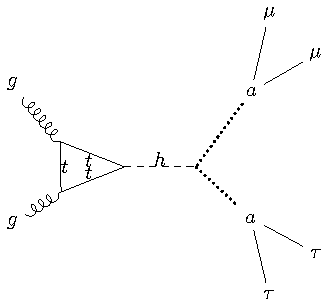
\includegraphics[width=0.47\textwidth]{figures/feynman_haa.pdf}
  \includegraphics[width=0.47\textwidth]{Figures/2m2t_BR_a40_t1-4.png}\\
    \caption{\label{fig:feynman_haa} Diagram of SM Higgs decay (denoted $h$ here) to pseudoscalar $a$ particles (Left) and branching ratios for pseudoscalar production in different $\text{tan}\beta$ scenarios and different 2HDM+S Types (right)}
\end{figure}

The branching ratios vary based on the value of $\text{tan}\beta$ depending on the type of model under investigation. In particular, Types I-IV are tested. Type III is expected to be most sensitive as it maintains a larger branching ratio compared to other decay modes over the range of the pseudoscalar masses when focusing on the final state of two muons and two tau leptons. In addition to the search for this model, any deviation from the SM prediction in the effective mass range would also be found.



\chapter{CERN, The LHC, and The CMS Detector}
\label{chap:cmsdet}
\section{CERN and the Large Hadron Collider}
The \textit{organisation européenne pour la recherche nucléaire} or CERN conducts the world's frontier particle physics experiments. 
Scientists at CERN represent numerous countries who work together for a greater understand of the universe. 
CERN hosts the Large Hadron Collider (LHC), currently the largest particle collider in the world. The LHC 27 km in circumference and holds eight experimental caverns 150 meters underneath the earth. Accelerator physicists and engineers strive to provide high energy collisions along these eight sites. More than 1500 superconducting magnets to steer and focus the accelerating protons. 
The beams are brought into collision at the four caverns where the experiments are sited.
%Crossing points facilitated by crab cavities force these particles to cross, collide, and interact at the caverns where the experiments take data. 
%Multiple campaigns for particle physics are done such as low intensity fills, lead-lead collisions, and proton collision. 
The LHC is capable of colliding both protons and heavy ions. 
The Compact Muon Solenoid (CMS) is the general purpose detector located at collision point 5(P5) in Cessy, France ~\cite{Bruning:782076}. 

\begin{figure}[ht!b]
  \centering
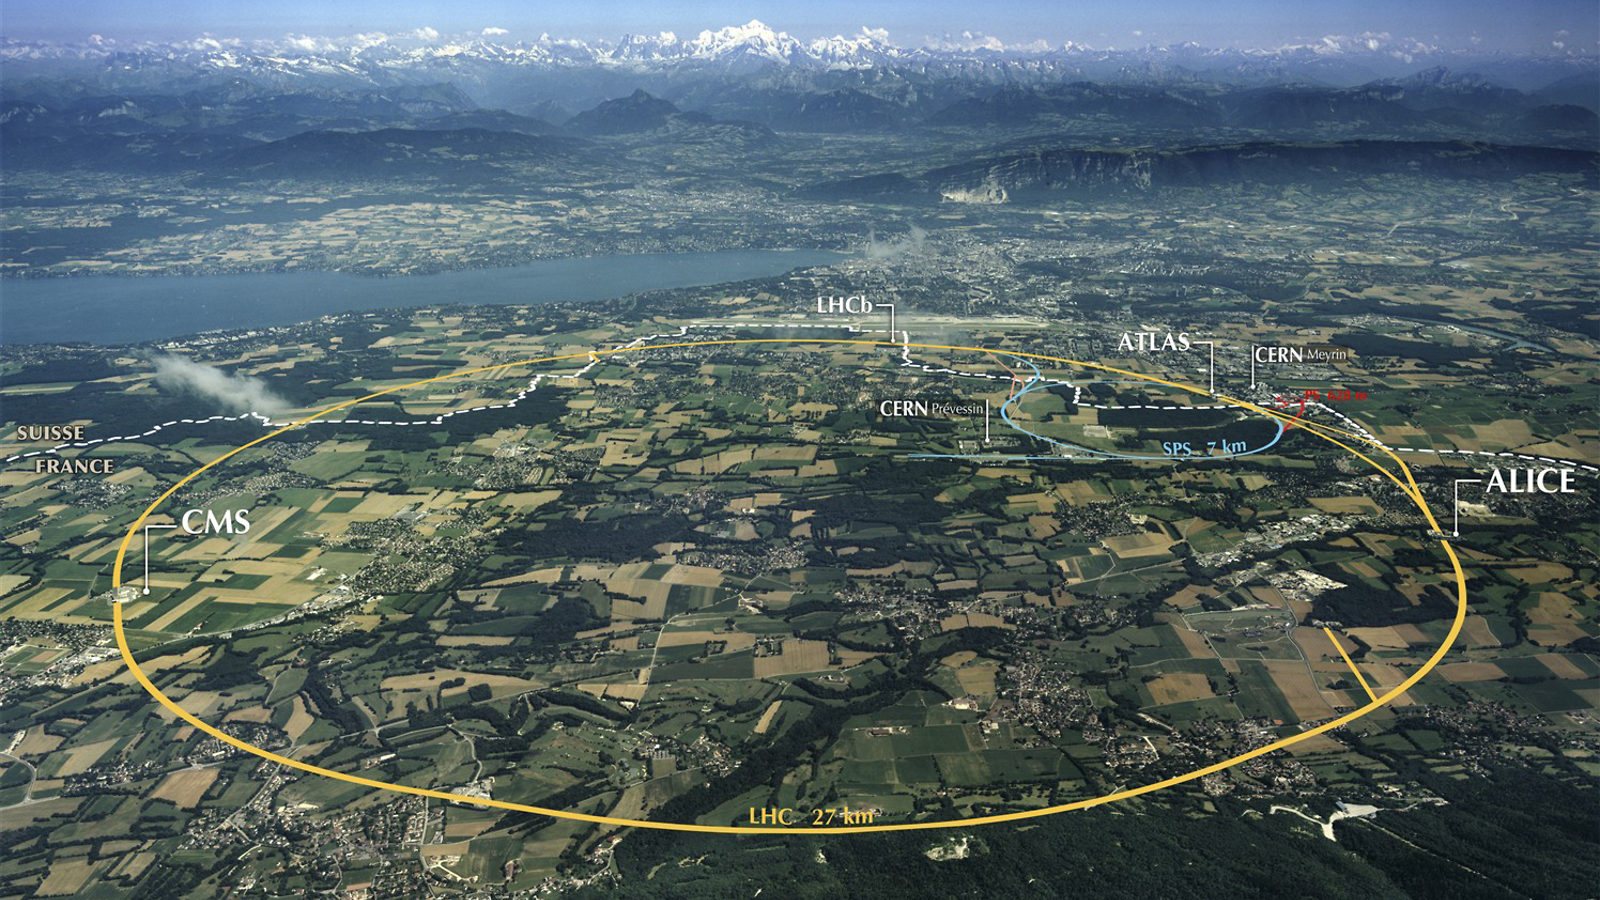
\includegraphics[width=0.75\textwidth]{figures/LHC_map-s.jpg}    
    \caption{\label{fig:lhc} Overview of the Large Hadron Collider spanning Switzerland and France - Maximilien Brice, CERN }
\end{figure}

\section{The Compact Muon Solenoid detector}
At around 14,000 tonnes, the CMS detector may not seem like it would be compact; however, it is quite dense. 
As shown in the diagram, the detector contains many subdetectors housed within a powerful solenoid magnet. At a diameter of 6 meters, a combined weight of 12,500 tonnes, and a field of 3.8 Tesla, the solenoid is the central feature of the Compact Muon Solenoid (CMS) \ref{fig:cmsdet}.
\begin{figure}[!htb]
\begin{center}
\includegraphics[width=0.75\textwidth]{Figures/cmsDet.png}
\caption{\label{fig:cmsdet}The CMS detector full 3D image with all subsystems labeled}
\end{center}
\end{figure}
 Within the solenoid volume, there is the
silicon pixel and strip tracker, a lead tungstate crystal 
electromagnetic calorimeter (ECAL), and a brass plus scintillator 
hadron calorimeter (HCAL). Each tracker and calorimeter comprises a barrel and two endcap 
sections. Forward calorimeters extend the pseudorapidity ($\eta$)
coverage provided by the barrel and endcap detectors. 
Muons are detected in gas-ionization chambers embedded 
in the steel flux-return yoke outside the solenoid.

A coordinate system centered on the nominal collision point is adopted. 
The $y$-axis points vertically outward toward the sky, the $x$-axis tangent to the Earth, and the $z$-axis along the direction of the beam pipe. The azimuthal angle $\phi$ and the radial coordinate $r$ in the $x$ and $y$ plane, and the polar angle $\theta$ measured from the $z$ axis are typically used to denote space points. 
Often pseudorapidity, defined by
\begin{equation}\eta = - \ln \tan(\theta/2)\end{equation}  
 is used to describe the angular distance from the beam pipe. 

%From the central interaction point, the CMS detector hosts
%the silicon pixel and strip tracker, the lead tungstate crystal electromagnetic
%calorimeter (ECAL), and the brass-scintillator hadron calorimeter (HCAL),
%each composed of a barrel and two endcap sections. The silicon pixel and tracking systems as well as
%the calorimeters are contained within the solenoid volume.  %cite

%The nominal $\Pp\Pp$ bunch crossing rate at the LHC is 40\unit{MHz}. This rate would be too extreme for any data taking system. In order to reduce the rate of events that are recorded for offline analysis, events of interest are selected using a two-step trigger system~\cite{Khachatryan:2016bia}.
%The first level (L1) is composed of custom built electronics which makes use of
%high speed optical links and large Field Programmable Gate Arrays (FPGAs). 

%L1 reduces the event rate from the nominal bunch crossing to a rate of aroun 100\unit{kHz} within a time interval of less than 3.5\mus.
%L1 reduces the rate from 40 MHz to 100 kHz.

%The second level, known as the High Level Trigger (HLT), consists of a farm of 
%generic processors running a version of the full event reconstruction software that
% has been optimized for fast processing. The HLT reduces the event rate to about
%1\unit{kHz} before data storage.

%Since the 2012 data taking, significant upgrades of the L1 trigger 
%have benefited this analysis, especially in the final state with two semi-hadronically decaying 
%$\Pgt$ leptons, denoted as $\tauh$.  
%These upgrades improved the $\tauh$ identification at L1 by giving more flexibility 
%to object isolation, allowing new techniques to suppress the contribution from 
%additional $\Pp\Pp$ interactions per bunch
%crossing, and to reconstruct the L1 $\tauh$ object in a fiducial region that matches 
%more closely that of a true $\tauh$ decay.

A more detailed description of the CMS detector can be found in Reference ~\cite{Chatrchyan:2008zzk}.

%In Phase 2, many upgrades are planned after Run III---which is currently on-going. 


\section{Subdetector Systems}
Several subdetector systems play an important role in the identification of the muons and tau leptons that are used in the analysis. 
While all subdetector systems are important to event reconstruction in CMS, there are several detectors that contribute to the particles that are identified in the pseudoscalar search. These are the tracker system, electromagnetic calorimeter, the hadronic calorimeter, and muon system. 

\subsection{Tracker}
%Working around silicon for almost 10 years, I have a slight bias in presenting this sub-detector system and I plan to share more details in this section than others. 

The tracker comprises several groups of silicon detectors. 
Going outward from the beam pipe, there is the pixel detector and then the silicon tracker.
A silicon detector works by sensing the ionization trail left by an energetic charged particle.
Typically, multiple band gaps are created through the process of lithography which adds artificial impurities of p-type (holes) or n-type (electrons). This process is known as ``doping". When a minimum ionizing particle (MIP) disturbs the latent charge---set by the bias voltage on the sensor---there is a current generated in the n and p type components which is given by the Shockley equation.
\begin{equation}
\label{eq:shockley}
\mathcal{J}_{n,p} = \frac{q_0 D_{n,p} d_{n,p}}{L_{n,p}}\left(e^{\frac{q_0 V}{k_B T}} - 1 \right)
\end{equation}
For reference: $L_{n,p}$ is the diffusion length, $D_{n,p}$ the diffusion coefficients, $d_{n,p}$ the charge/hole density, $V$ the bias voltage, $q_0$ the standard charge unit, $k_B$ the Boltzmann constant, and $T$ the temperature. 
This current is sensed by the electrodes etched onto the silicon substrate. 
A graphical display of surface current using simulation as a function of time is shown in figure \ref{fig:sd}. A wealth of silicon information can be found in reference ~\cite{Eichhorn:2112017}.

\begin{figure}[ht!b]
  \centering
  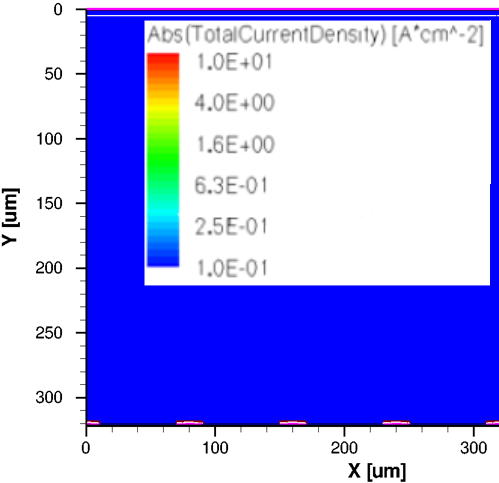
\includegraphics[width=0.31\textwidth]{figures/silicon/silicon_t0.0.png}
  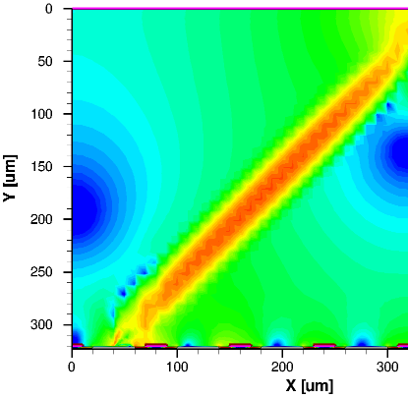
\includegraphics[width=0.31\textwidth]{figures/silicon/silicon_t1.1.png}
  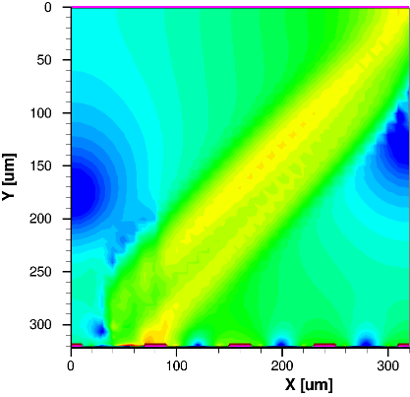
\includegraphics[width=0.31\textwidth]{figures/silicon/silicon_t1.5.png}\\
  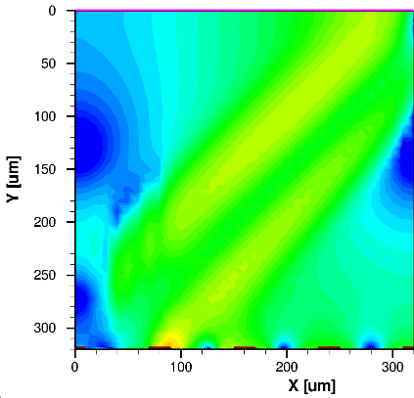
\includegraphics[width=0.31\textwidth]{figures/silicon/silicon_t2.0.png}
  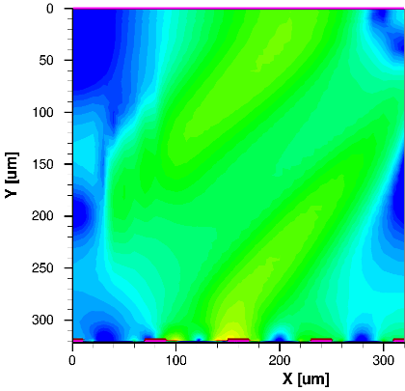
\includegraphics[width=0.31\textwidth]{figures/silicon/silicon_t3.0.png}
  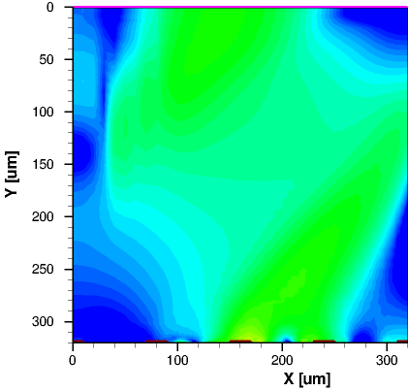
\includegraphics[width=0.31\textwidth]{figures/silicon/silicon_t4.0.png}\\
  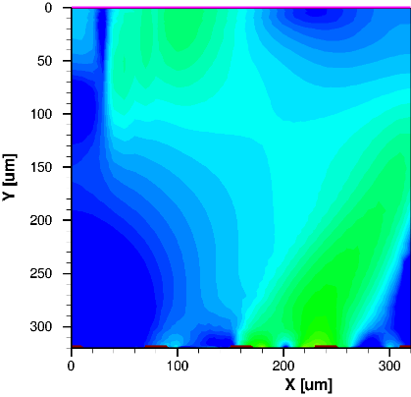
\includegraphics[width=0.31\textwidth]{figures/silicon/silicon_t5.0.png}
  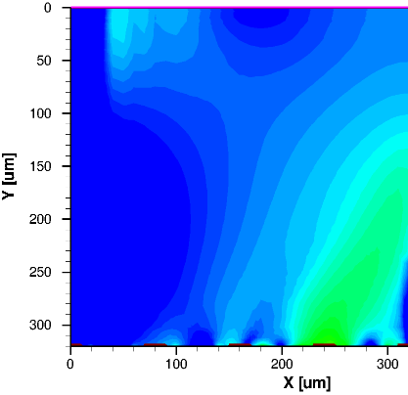
\includegraphics[width=0.31\textwidth]{figures/silicon/silicon_t6.0.png}
  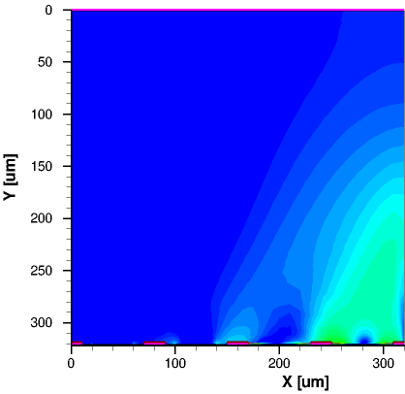
\includegraphics[width=0.31\textwidth]{figures/silicon/silicon_t7.0.png}\\
    \caption{\label{fig:sd} (simulation) MIP particle traveling across a silicon strip sensor at $45^\circ$ over time from 0.0, 1.1,1.5,2,3,4,5,6,7 nanoseconds. The induced surface current dissapates and would be collected by the channels of the silicon module ~\cite{Eichhorn:2112017}.}
\end{figure}





\subsubsection{Pixel Detector}
\label{sec:pixeldet}
The pixel detector contains the Barrel Pixels (BPIX) and the Forward Pixels (FPIX).  
Similar $2\times8$ silicon detector modules make up both the BPIX and FPIX systems.

In 2016, the phase 1 Forward Pixel System (FPIX) was constructed and tested. At Purdue University, an Aerotech robotic gantry control system was used to join a hybrid flex circuit to a bump-bonded silicon pixel module. After wirebonding, the gantry system encapsulated the wirebonds for protection from corrosion and magnetic field resonance. Purdue was one of the manufacturing sites alongside University Nebraska-Lincoln. 

Using LabVIEW, we developed a state machine to assemble and encapsulate these pixel modules. Pattern recognition and a linear algebra suite were developed to perform precise operations at a 50 micron resolution. An example of a post encapsulated token bit manage--which resides on top of the high density interconnect of a completely assembly module---is shown in figure \ref{fig:tbm}.

\begin{figure}[ht!b]
    \centering
  \includegraphics[width=0.65\textwidth]{fpixtbm.jpg}
    \caption{\label{fig:tbm} encapsulated token bit manager of a forward pixel module currently installed in CMS}
\end{figure}


In 2017, this system was installed in CMS, increasing the number of disks to three and the number of barrel layers to four.  The design of CMS is such that the inner sub-detector systems may be taken out of the solenoid and serviced.  
These forward disks, which are especially important for the reconstruction of boosted charged particles, are located in high regions of $\eta$ and are overlapped for improved hermeticity.  


\subsubsection{Silicon Tracker}
The silicon tracker comprises larger silicon modules by area than the pixel system and is located further from the beam pipe. A representative layout of the silicon tracker and the pixel system can be found in figure \ref{fig:tracker} ~\cite{Chatrchyan:2008zzk}. 

\begin{figure}[ht!b]
\label{fig:tracker}
  \centering
  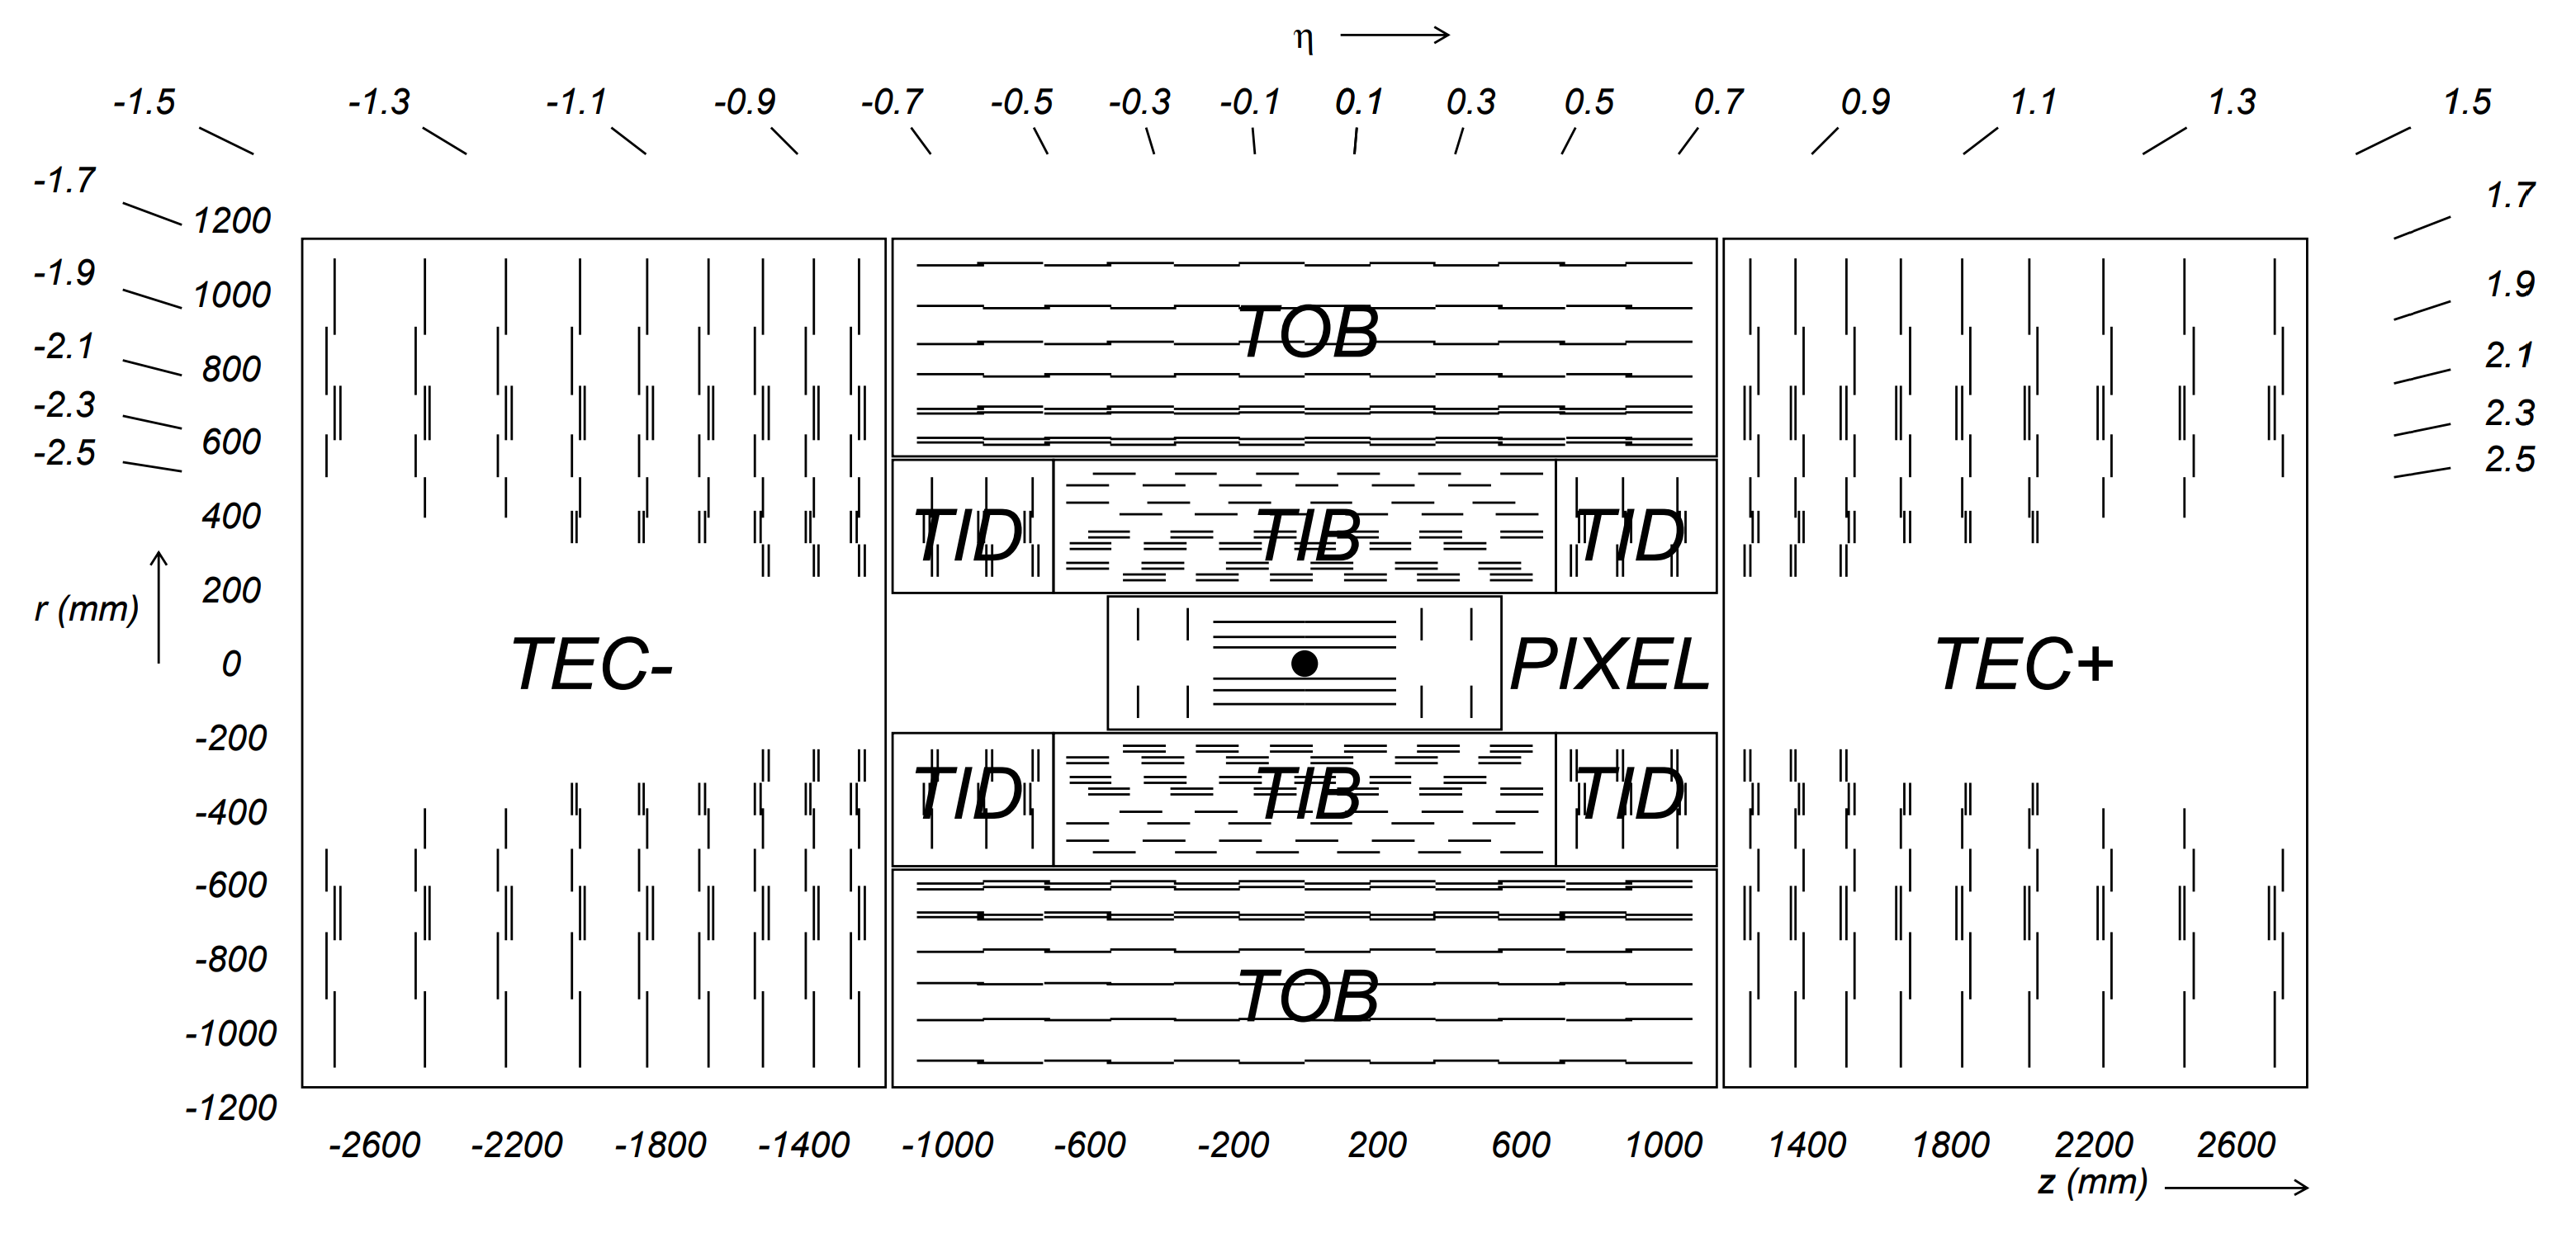
\includegraphics[width=0.85\textwidth]{figures/silicon/SiliconTracker.png}\\
    \caption{ The silicon tracker system, consisting of the inner pixel system (BPIX and FPIX), The Tracker End Caps (TEC), Tracker Inner Detector(TID), Tracker Inner Barrel (TIB), and the Tracker Outer Barrel (TOB) by position in r, z , and $\eta$ ~\cite{Chatrchyan:2008zzk}}
\end{figure}



\subsection{Electromagnetic Calorimeter (ECAL)}

The principal components of the ECAL are the 76200 lead tungstate ($\text{PbWO}_4$) crystals, which scintillate and absorb energy from incoming particles. These detector components are also separated in barrel and endcap regions. A photomultiplier is attached to each the crystal to detect its light signal. The relative energy resolution is 
\begin{equation*}
\label{eq:ecal}
\left(\frac{\sigma}{E}\right)^2 = \left( \frac{2.8\%}{\sqrt{E}}  \right)^2 + \left( \frac{0.12}{E}  \right)^2 + (0.3\%)^2 
\end{equation*}
 The first, second, and third terms in equation \ref{eq:ecal} reflect the stochastic, noise, and constant terms as determined in the calibration run with a 440 nm blue laser ~\cite{Chatrchyan:2008zzk,Eichhorn:2112017}. 

\subsection{Hadronic Calorimeter (HCAL)} 
The Hadronic Calorimeter is the primary sub-detector to identify ``jets", which are collimated collections of hadrons. 
Brass plates interwoven with plastic scintillators are used to induce particle showers. 
Light signals from the scintillators are propagated through wavelength shifting fibers and read out through an optical decoding unit, before ultimately landing at a hybrid photodiode. 
There are barrel (HB) and endcap (HE) inside the solenoid. The Hadronic Outer (H0) and super forward detector (HF) sit outside the solenoid. An overview of the HCAL system is shown in figure \ref{fig:hcal} ~\cite{Chatrchyan:2008zzk,Eichhorn:2112017}. 

\begin{figure}[ht!b]
  \centering
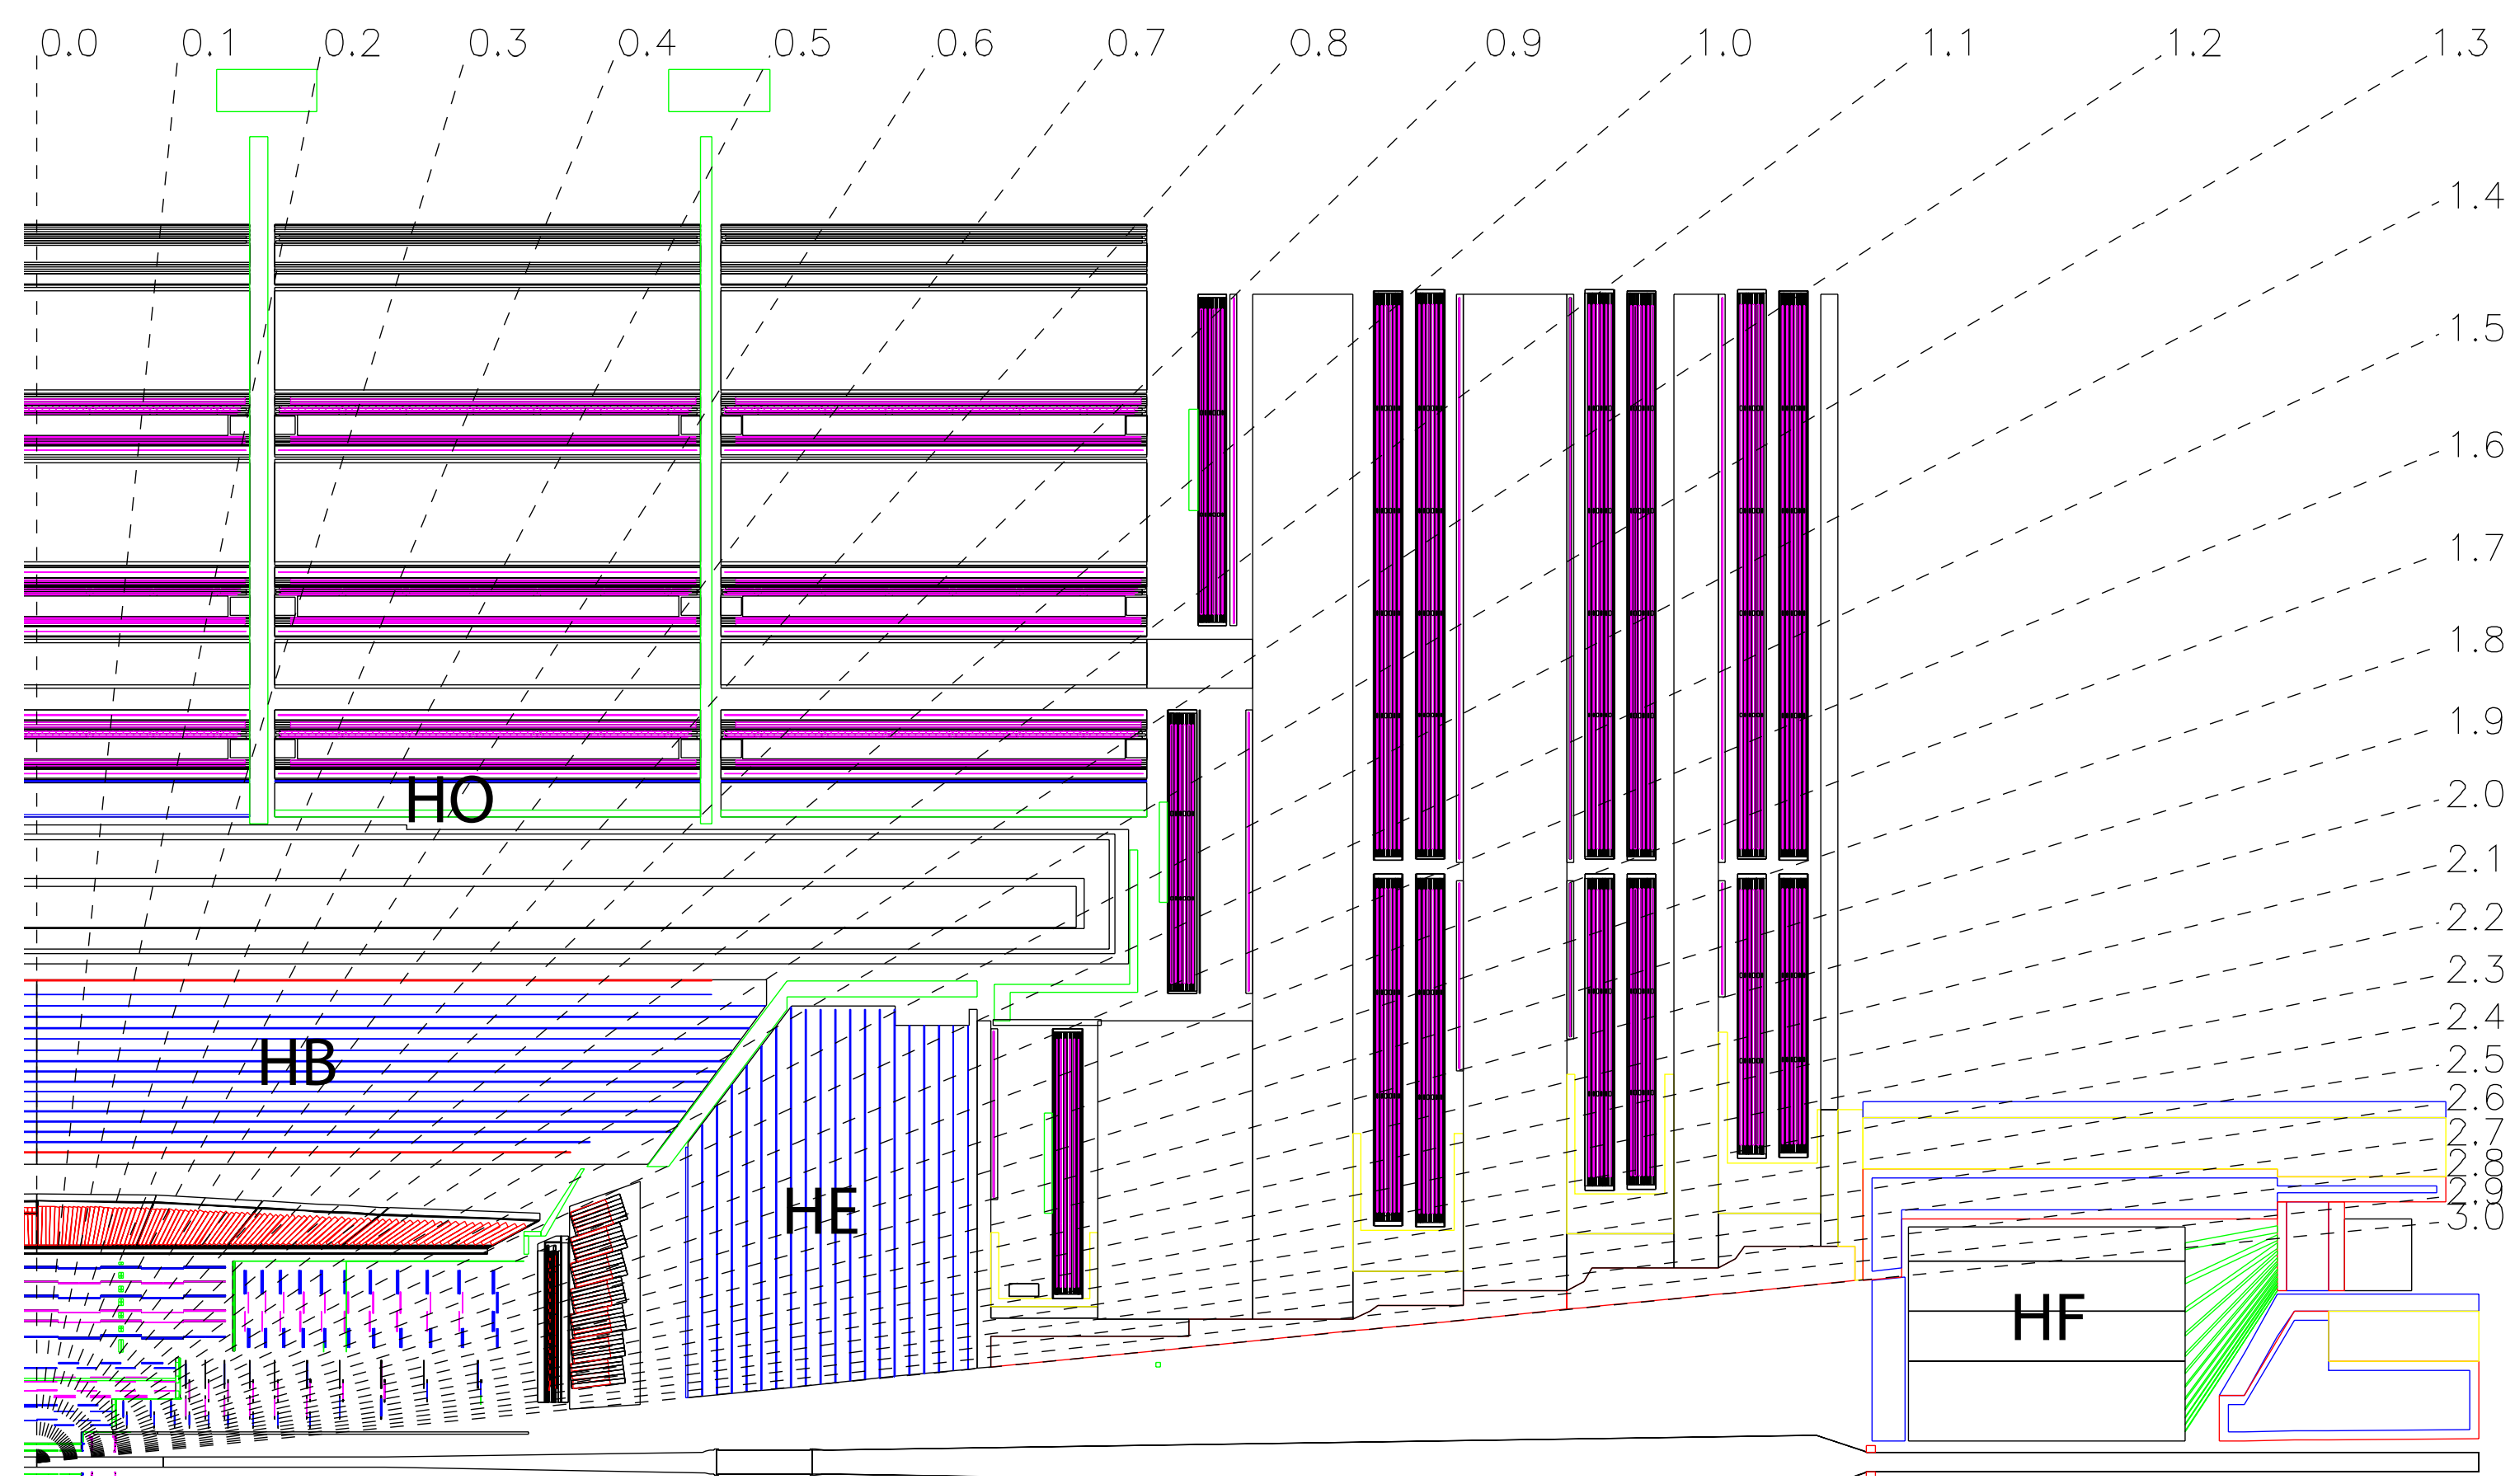
\includegraphics[width=0.85\textwidth]{figures/HCAL.png}    
    \caption{\label{fig:hcal} Overview of the HCAL system from the z---$\eta$ plane showing the hadron barrel (HB), encap(HE), outer (HO), and the forward (HF) subsystems ~\cite{Chatrchyan:2008zzk}}
\end{figure}




\subsection{Muon System} 
The muon system comprises drift tubes which cover a pseudorapidity region ($|\eta|<1.2$) split into four stations interleaved in the flux return plates.
In the higher $|\eta|$ endcap regions, cathode strip chambers (CSCs), which provide fast response time, fine segmentation, and radiation resistance, are used ~\cite{Chatrchyan:1129810}. For a visual representation of a cross section of the muon system please refer to figure ~\ref{fig:muonsystem}. 
Notably, the track of the muon is bent inside the solenoid by the Lorentz force, and then reverses after it exits. 

\begin{figure}[ht!b]
  \centering
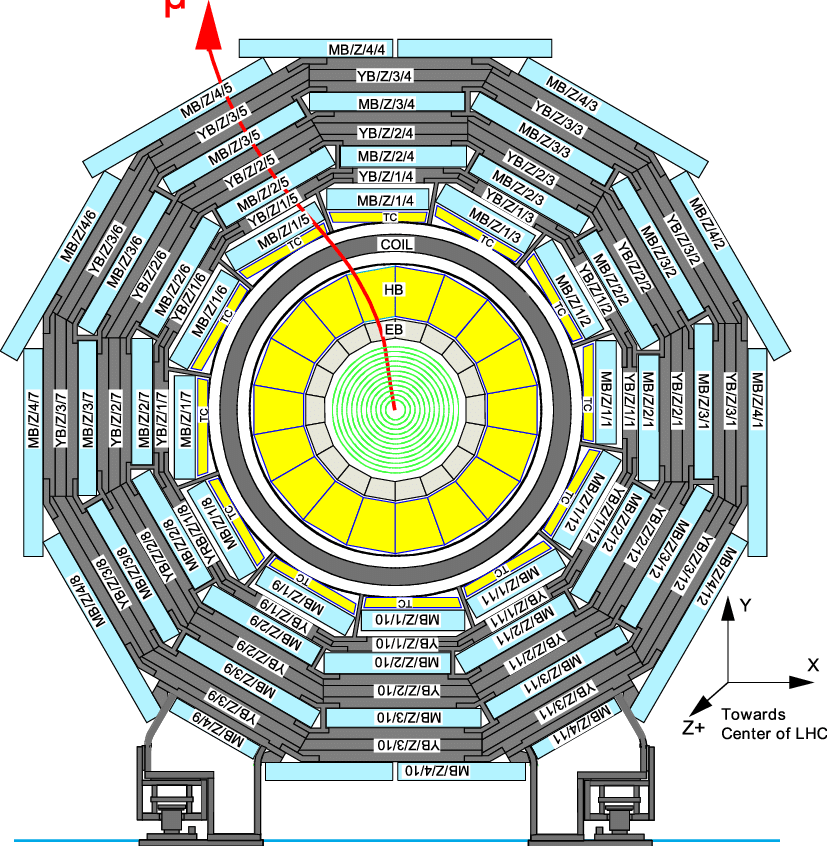
\includegraphics[width=0.75\textwidth]{figures/Layout-of-the-CMS-barrel-muon-DT-chambers-in-one-of-the-5-wheels-59.png}    
    \caption{\label{fig:muonsystem} Muon system involving multiple subdetector systems: tracker, solenoid, and the muon gas chambers around the iron yoke (grey) - Maximilien Brice, CERN }
\end{figure}


\section{Level 1 Trigger System and High Level Trigger}
Particle collisions happen at a rate of 40 MHz with each bunch crossing, resulting in about 20 minimum bias events. The bandwidth that would be needed to record all these collisions is prohibitively high ~\cite{Bruning:782076,Foudas:2232067}. The Level 1 trigger (L1) and High Level Trigger (HLT) work to reduce these rates by selecting events of interest. 

The L1 trigger system, which comprises many subsystems,can process data at the beam collision rate. Algorithms are in place that take input from the calorimeters, the muon systems, and other detectors in the form of ``trigger primitives'' and use pattern recognition, along with fast summing techniques, to trigger on the event. Many of these algorithms are run on Field Programmable Gate Arrays (FPGAs). 
After 144 beam crossings, the Global Trigger (GT) initiates readout for events of interest at the front end electronics. 
 The L1 system also outputs physics objects to seed the reconstruction algorithms used by the HLT ~\cite{Foudas:2232067}. 
The HLT maximum input rate is 100~kHz and the output is on the order of kHz. It is constrained by the processing power available, the data recording and transfer rate of Tier 0, and the prompt reconstruction algorithms. Late in Run II  ``Scouting'' and ``Parking'' data were used to make more efficient use of the available bandwidth. Scouting reduces the event size by saving only objects reconstructed by the HLT. Parking reduces the immediate load on the T0 system by postponing prompt reconstruction to a time when CMS is not running ~\cite{Thomas:2703017}.


\section{Particle Flow Algorithms}
The event data model requires association of higher level physics objects---like leptons---with energy deposits and tracks in the detector. 
The particle flow algorithm at CMS has the goal of associating these primary detector signatures with these particles so that direct comparison to Monte Carlo simulation can be done. 
The list of particle objects includes jets, missing transverse energy, taus, charged-leptons, photons, and bottom quark jets among others.
To outline the algorithm: charged particle tracks reconstructed in the tracker, energy clusters from the ECAL, HCAL, and preshower detector (ES), and forward calorimeter (HF) are topologically linked into blocks. The linking is done through many associations of energy deposits and tracks in $\phi,\eta$ space. These blocks are then interpreted as particles. Further details can be found in reference ~\cite{CMS-PAS-PFT-10-001}.

\section{Computational Infrastructure}
Over 200 peta-bytes of information have been gathered in Run II. A schematic overview of the computing infrastructure can be found in figure \ref{fig:t0} ~\cite{Hufnagel:1319049}.

\begin{figure}[ht!b]
  \centering
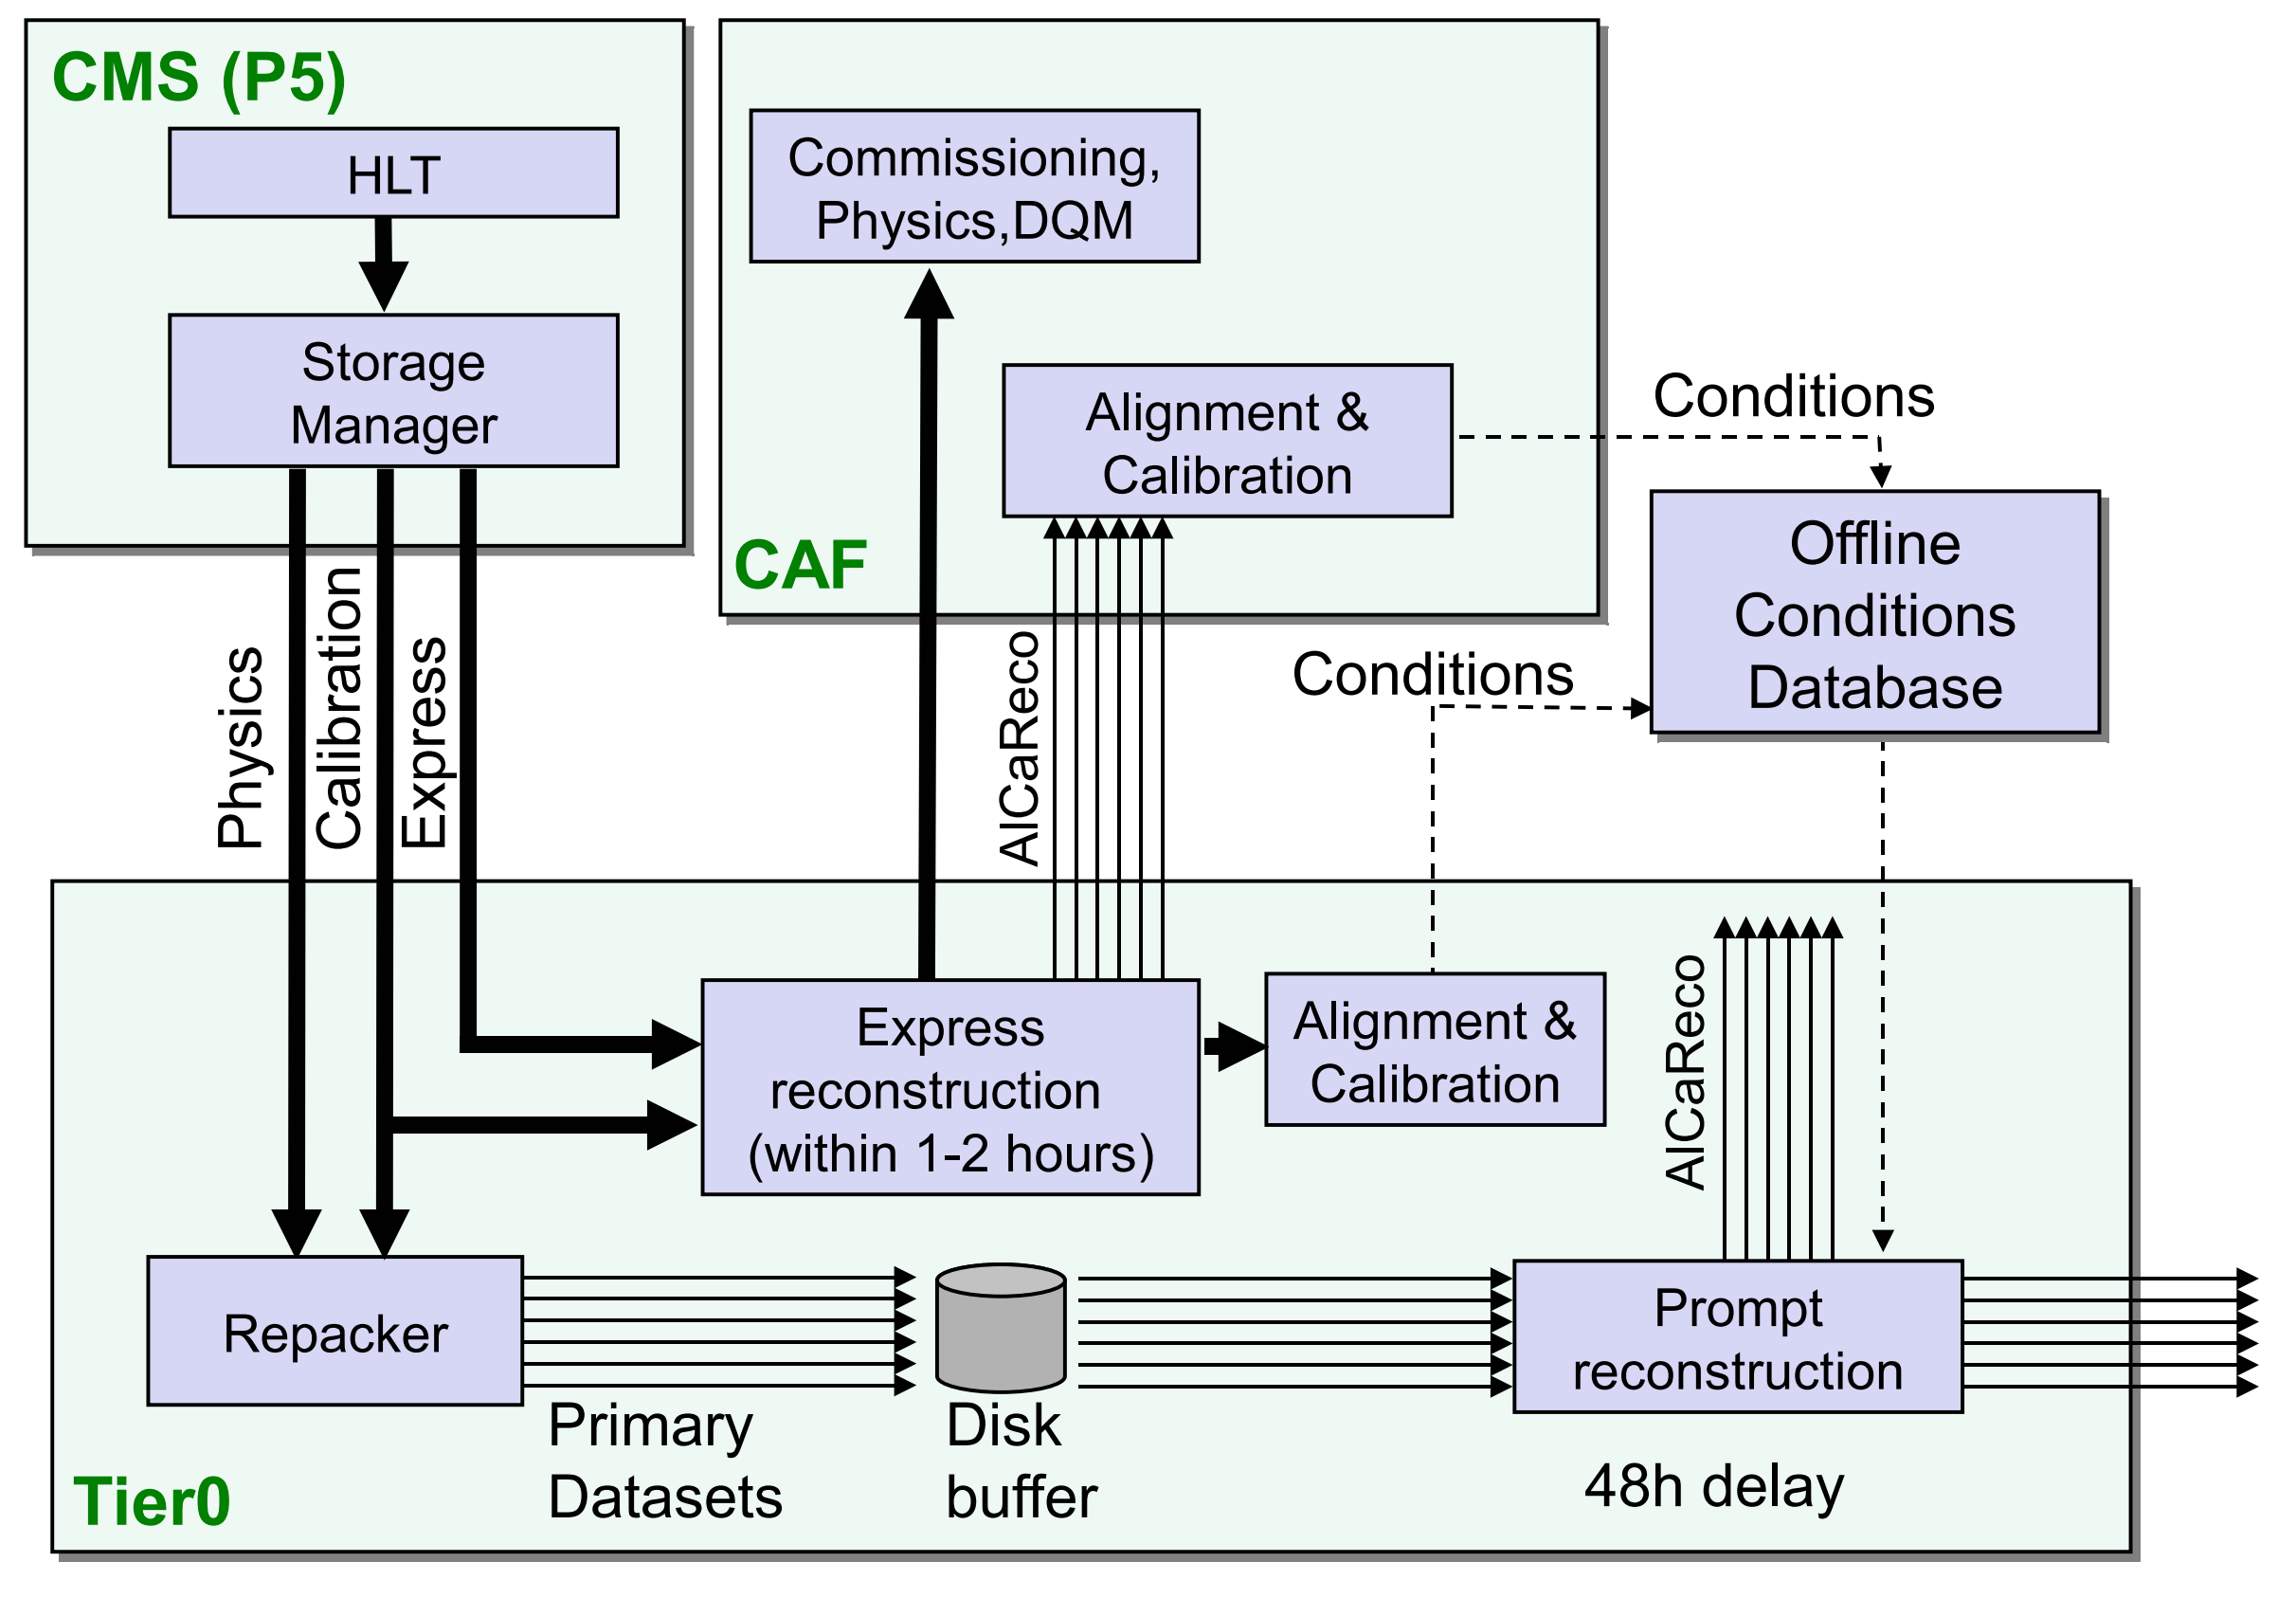
\includegraphics[width=0.75\textwidth]{figures/Tier0.png}    
    \caption{\label{fig:t0} Schematic overiew of Tier0 computing, data can be available from different sections allowing for data quality monitoring and also storage to several databases ~\cite{Hufnagel:1319049} }
\end{figure}

The Tier 0 (T0) facility which comprises 32,000 24-core processors is where higher level reconstruction of physics objects is done.  
The data are stored and processed at many different sites, organized by tiers. There is one Tier-0, seven Tier-1, about one-hundred fifty Tier-2, and numerous Tier-3 centers. The sum of these tiers is the ``grid'' or the Worldwide LHC Computing Grid (WLCG), which in total combines 900 000 CPUs from over 170 sites in 42 countries. Tools like \texttt{XrootD} and \texttt{Rucio} allow physicists from around the world to access centrally supported data. An abundance of up to date information can be found \texttt{https://home.cern/science/computing/grid}. 





\chapter{Luminosity}
\label{chap:lumi}
\section{Luminosity at the LHC}
Luminosity sets the scale for the number of events recorded at the LHC. It is how bright the beam is and dictates how many interactions can be expected over a data taking period. Therefore, it is important for all physics analyses to use the correct luminosity, and its measured error, to obtain an accurate result. The number of expected events for any given process is the luminosity $\mathcal{L}$ times the cross section $\sigma$.  
\begin{equation}
N_{\text{event}} = \mathcal{L} \sigma_{\text{event}}
\end{equation}
\begin{equation}
\mathcal{L} = \frac{N_b^2 n_b f_\text{LHC} \gamma_r}{4\pi\epsilon_n \beta*}\left( 1 / \sqrt{1+ (\frac{\theta_c \sigma_z}{2\sigma*})^2} \right)
\end{equation}

$N_b$ is the number of particles in the bunch crossing, $n_b$ the number of bunches, $f_{\text{LHC}}$ the revolution frequency of the LHC, $\gamma_r$ the relativistic factor, $\epsilon_n$ the normalized beam emmittance, $\beta*$ the beta function at the collision point (related to the crossing angle), $\theta_c$ is the full crossing angle, $\sigma_z$ the RMS bunch length and $\sigma^*$ the transverse RMS beam size at the interaction point.

\section{Luminometers}
Several subsystems are used to measure luminosity at CMS. Particularly, the Pixel Luminosity Telescope, HF with summed transverse energy (ET) and occupancy (OC), BCM1F, and Tracker/Pixel based luminosity detectors to name several. 
In this section, the tracker based luminosity will be the focus. The pixel system is integral in the reconstruction of events for physics analyses and in measuring the luminosity.

There was calibration of the new pixel detector in early 2017, from the BPIX and FPIX upgrades mentioned in section \ref{sec:pixeldet}. The Lumi-POG---Luminosity physics object group---commisioned luminosity measurement using the clusters from the new pixel detector in an automated workflow. 
%Taking many local hits in the pixel module - a.k.a. a pixel cluster - 
We measure the luminosity by counting pixel clusters in a low channel occupancy setting and scaling it by a visual cross section---the measured cross section for the instrument---determined in a separate analysis. Using the relation in equation \ref{eq:pcclum}, the instantaneous luminosity can be obtained once the number of clusters and the visible cross section $\sigma_\text{cluster}$ are measured. 
\begin{equation}
\label{eq:pcclum}
\langle N_{\text{cluster}}\rangle\equiv\frac{\sigma_{\text{cluster}}}{f_{\text{LHC}}}\mathcal{L}_{\text{SBIL}}
\end{equation}

$\mathcal{L}_{\text{SBIL}}$ is the instantaneous luminosity of a single bunch crossing---the aggregate collection of protons that are in the beam typically 3564 total bunches during standard pp-collisions. $\sigma_{\text{cluster}}$ is the cross section that is measured in a separate analysis involving Van-de-Meer scans (beam dynamic scans). More details can be found here ~\cite{Knolle:2792593}. 


\subsection{Tracker luminosity}
For the pixel luminosity, a two component correction is applied on the fly to correct for self-radiative effects on the pixel modules under particle fluence and for inefficiencies.  
One detail that is important in estimating the luminosity from the pixel detector is ensuring that the data that is taken and analyzed has consistent performance. Several times in a year, the Lumi-POG and Beam Radiation Instrumentation Luminosity (BRIL) groups analyze the performance of each subdetector used to measure luminosity and certify the data once the analysis is complete. In 2017 and 2018 data taking campaigns, the luminosity from the pixel detector was vetted by looking at relative module performance over the runs of data taking for those years. If the modules didn't have consistent performance, they were removed from the final result. 

Even though up to half of the modules were vetoed after this procedure, there was plenty of statistics due to high numbers of pixel clusters per event. 
This module veto decision was made by taking the total clusters in each module and scaling them so that the overall total clusters are one. Then, on a per-module basis, the performance relative to the total clusters was compared. This helped the analyzer look at consistent performance and manage a list of passing modules used in a final luminosity measurement using the pixel detector. 

For Run III data taking, integration of the cluster counting procedure was included at the HLT. A data compression of $10^3$ was made by taking the low level data from the silicon pixels and storing them in a simple data container, which saved a peta-byte of data. Luminosity measurements using these data containers and methods are being investigated as more CMS-physicists are interested in using the central tracking system for luminosity measurements.






\chapter{Lepton Identification and Object Selection}
\label{chap:samples}

\section{Lepton identification}
The following three sections briefly describe how certain subsystems of the CMS detector work together to identify muons, electrons, and tau leptons. 

\subsection{Muon identification systems}

As CMS implies in its name, muons are certainly a focal point in particle detection. 
Looking at muons that come from the interaction vertex---prompt muons---the tracker plays an important role in identifying charged particle tracks. 
The tracker system works in conjunction with the gas chambers to reconstruct muons, and the solenoid bends the muon's tracks allowing the momentum to be measured for an accurate mass resolution. By design, muons should be the only particle that should reach the gas chambers, making for great muon efficiency. 
During reconstruction, muons are identified and are ultimately divided into four working points (very loose, loose, medium, tight). These points are defined based on their efficiencies and depend on the $\chi^2$ of the track and momentum of the candidate muon ~\cite{CMS-PAS-PFT-09-001,Kratschmer:1956760}.


\subsection{Electron identification systems}
The main subdetector involved with electron identification is the ECAL. To identify electrons, a cluster of energy in the ECAL is associated with a track that is constructed in the silicon detector system. 
The tracks are identified in the typical fashion using the Kalman Filter tracking technique to pick good quality tracks, and then the tracks are refitted using a Gaussian Sum Filter. 
These tracks are then associated with an ECAL super cluster---grouped energy deposits---by requiring matching in $\eta,\;\phi$ space
\begin{equation}|\Delta\eta| = |\eta_{\text{SC}} - \eta_{\text{in}}^{\text{extrap}}| < 0.02\end{equation}
\begin{equation}|\Delta\phi| = |\phi_{\text{SC}} - \phi_{\text{in}}^{\text{extrap}}| < 0.15\end{equation}
This method has an overall efficiency of about 93\% ~\cite{Khachatryan:2015hwa}. 

\subsection{Tau identification systems}
Tau leptons decay in many different ways. It is the heaviest lepton, so heavy it can decay to intermediate mesons such as the $\rho$, $a$, and $\pi$ mesons.
Ergo, when it comes to tau identification, many algorithms are needed to properly identify them using information across the detector. 
Tau leptons decay both hadronically and leptonically as shown in the table \ref{tab:taudecay} below. 



\begin{table}[h!tbp]
\centering
    \topcaption{Possible hadronic tau decays, $h$ doesn't indicate a Higgs particle but a hadronic prong~\cite{Workman:2022}}
\label{tab:taudecay}
\begin{tabular}{c c r}
Decay Modes & Resonance & \multicolumn{1}{c}{$\mathcal{B}(\%)$} \\\hline
Leptonic Decay && \multicolumn{1}{l}{35.2}\\
$\tau^- \rightarrow e^- \bar{\nu}_e \nu_\tau $ & & 17.8 \\
$\tau^- \rightarrow \mu^- \bar{\nu}_\mu \nu_\tau$ & & 17.4 \\\hline
Hadronic Decay && \multicolumn{1}{l}{64.8}\\
$\tau^- \rightarrow h^-\nu_\tau$ & & 11.5 \\
$\tau^- \rightarrow h^-\pi^0 \nu_\tau$ & $\rho(770)$ & 25.9 \\
$\tau^- \rightarrow h^-\pi^0 \pi^0 \nu_\tau$ & $a_1(1260)$ & 9.5 \\
$\tau^- \rightarrow h^- h^+ h^- \nu_\tau$ & $a_1(1260)$ & 9.8 \\
$\tau^- \rightarrow h^- h^+ h^- \pi^0 \nu_\tau$ & & 4.8 \\
Other & & 3.3 \\\hline
\end{tabular}
\end{table}

%The important algorithms directly related to hardware are the Hadron Plus Strips (HPS) algorithm which combines the use of the tracker system and the electromagnetic calorimeter (ECAL) for hadronic tau identification ~\cite{Sirunyan_2018}.  

The Hadron Plus Strips (HPS) combines the use of the tracker system and the electromagnetic calorimeter (ECAL) for hadronic tau identification ~\cite{Sirunyan_2018}.  


 


\section{Data and simulation}
For this analysis, muons are paramount, so there must be a certain number of muons triggered for the event to be selected. Two final states contain electrons, so datasets containing electrons are also used. The single muon, double muon, and electron plus photon datasets are used depending on the year. These datasets contain the triggers that are the most important for object selection. Single muon triggers that contain isolated muons at 22, 24, and 27 GeV thresholds are implemented, along with double muon triggers with good reconstructed muons at a 17 GeV threshold. More information on triggers and selection is given in the event selection section ~\ref{sec:trig}. 

The simulation typically used to compare with data is MadGraph5@NLO with PYTHIA 8 for hadronization \cite{PYTHIA}. These CMS centrally-generated samples are then digitized using GEANT4 \cite{GEANT4} to the same format as real data events collected and processed at CMS HLT. This raw data is then reconstructed to physics objects---such as tracks and higher level objects like leptons. A direct comparison between data and simulation can be made after calibrating simulation in control regions. 

Data taken from CMS during the entire Run II period was examined, corresponding to 137 $\text{fb}^{-1}$ of integrated luminosity. The list of data and simulation Monte Carlo (MC) is exhaustive and listed in the appendix \ref{app:data}.   

For the MC production of the signal samples, to reflect the 2HDM modeling, events were generated at tree level for a pseudoscalar Higgs like boson between the masses of 15 and 60 GeV in intervals of 5 GeV with the parent Higgs produced through gluon fusion. These masses are sufficient for the parametric modeling, which is used in the fit model, to obtain a precise peak resolution ~\ref{sec:fitmodel}. Signal samples were produced centrally by CMS for 2016, but privately produced for 2017 and 2018. The scripts and conditions used are located here:\\
 \texttt{https://github.com/samhiggie/iDM-analysis-AODproducer/tree/haa} .\\
The NMSSMHET model was used to simulate the events. Parameters and information can be seen in the package:
https://cms-project-generators.web.cern.ch/cms-project-generators/ .



\section{Physics object selection} 
\label{sec:objsel}
%Baseline selections are recommended by the various Physics Object Groups (POGs) for object selection. Ultimately, these take the form of cuts for leptons based primary on kinematic variables like the momentum. 
Baseline selections for objects are recommended by the various Physics Object Groups (POGs). The process of making selections on variables is known as ``making cuts". Ultimately, these take the form of cuts for leptons based primary on kinematic variables like the momentum. 
Selections are made to identify muons, electrons, and tau leptons. These three leptons form the objects under selection and comprise the final states in the analysis.
All leptons under consideration must pass trigger requirements that depend on momentum of the lepton. Special triggers are used for the different final states depending on the number of muons in the event. A precise description of the triggers used are given later in section ~\ref{sec:trig}.
Identifying particles in object selection is critical, particularly differentiating between lepton candidates that come from the interaction vertex (prompt) and those that appear from decays down the line (nonprompt). Relative isolation is typically defined in order to ensure there is no overlap between candidate leptons, to make sure that each lepton is not associated with other physics objects like jets. More details on this variable and it's usage in the Particle Flow algorithm can be found here  ~\cite{Sirunyan_2017}. 
\begin{equation}
I^{\ell} \equiv \frac{\sum_\text{charged}  \PT + \max\left( 0, \sum_\text{neutral}  \PT
                                         - \frac{1}{2} \sum_\text{charged, PU} \PT  \right )}{\PT^{\ell}}.
\label{eq:reconstruction_isolation}
\end{equation}
$\sum_\text{charged}  \PT$ is the scalar sum of the
transverse momenta of the charged particles originating from
the primary vertex and contained in a cone of size
$\Delta R = \sqrt{\smash[b]{(\Delta \eta)^2 + (\Delta \phi)^2}} = 0.4$\,(0.3)
centered on the muon (electron) direction. The sum $\sum_\text{neutral}  \PT$ is
a similar quantity for neutral particles. Track association isn't possible with neutral particles and thus not with primary vertex information; therefore, to take pileup into consideration, an estimate of the transverse momentum from the pile up contribution is subtracted (PU $\PT$).  

As mentioned in the instrumentation and detector chapter~\ref{chap:cmsdet}, the muon identification system uses the tracker to identify charged tracks and the muon chambers to identify the particles later in their trajectory after they exit the solenoid. Typically, ``good" muons are those that are both associated with a track and their subsequent identification in the drift tubes, CSCs, or RPCs. The average muon lifetime is 2.2 $\mu$s so they travel quite far from the interaction point.  The physics object group's recommendations are followed, which select muons with $\pt>15\GeV$ and $\abs{\eta}<2.4$ in addition to selecting only ``good" muons.

Electrons originating from the tau decay are reconstructed by track association along with energy deposition in the Electronic Calorimeter (ECAL). Events are vetoed for candidate electrons that also show a substantial energy deposition in the HCAL for better efficiency. The hits and track quality from two separate algorithms, along with the geometrical and energy matching from the ECAL are used in a Multivariate Analysis (MVA) technique to select good electrons for analysis 
~\cite{Khachatryan:2015hwa}.

To identify $\tauh$ candidates, the hadron-plus-strips (HPS) algorithm is used to identify the major modes of the hadronic tau decay ~\cite{Sirunyan_2018}. Typically, events with hadronic prongs---charged hadrons---are considered in combination with a number of neutral pions and missing transverse energy from the neutrinos. Neutral pions almost always decay to photons, so a hadronic tau identification algorithm should combine the identification of charged hadrons and neutral pions. 
The hadron plus strips (HPS) algorithm combines inner track information, hits in the HCAL, and pion association in the ECAL by deposits in a $\eta,\phi$ strip region to identify hadronic tau leptons. 
The $\tauh$ is matched to $h^{\pm}$, $h^{\pm}\pi^{0}$, $h^{\pm}h^{\mp}h^{\pm}$, or $h^{\pm}h^{\mp}h^{\pm}\pi^{0}$ depending on the overall charge vs neutral constituents ~\cite{Sirunyan:2018pgf,Hassanshahi:2797703}.
In addition to the HPS algorithm, a Deep Neural Network (DNN) was constructed to further aid in identification by discriminating between genuine tau leptons and those that originate from quarks or gluon jets, electrons, or muons.  
In the DNN, the tau four-momentum and charge,
the number of charged and neutral particles constituents,
the isolation variables,
the compatibility of the leading tau track with the primary vertex,
the properties of a secondary vertex in case of a multiprong tau decay,
observables related to the $\eta$ and $\phi$ distributions of energy reconstructed in the ECAL strips,
observables related to misidentified taus as electrons, 
and the estimated pileup density in the event are all used. In total, 47 high-level input variables are incorporated 
~\cite{https://doi.org/10.48550/arxiv.2201.08458}.
In practice, the DNN has discriminators against muons, electrons, and jets that fake genuine taus and has efficiencies that go from 40\% to 90\%, in a 10\% granularity of the discriminating variable. The medium working point is used for each of these discriminators. 
All leptons also have a momentum threshold and isolation requirements to place them in a kinematic region where good agreement between data and MC is expected in control regions.  

\begin{table}[h!tbp]
\centering
\topcaption{$t\bar{t}$ baseline cuts and identification for lepton selection $\delta Z$ and $\delta xy$ are distances from the interaction vertex
\label{tab:basecuts}
}
\begin{tabular*}{0.8\textwidth}{c|p{0.6\linewidth}}
\hline
lepton          & baseline cuts \\\hline 
Muon            & $\delta Z < 0.2$, $\delta xy < 0.045$, $\pt > 5.0 GeV$, $\text{Iso.} <= 0.2$, $\eta \geq 2.4$\\\hline
Electron        & $\delta Z < 0.2$, $\delta xy < 0.045$, $\pt > 7.0 GeV$, $\text{Iso.} <= 0.15$, $\eta \geq 2.5$ \\\hline
Tau             & $\delta Z < 0.2$, $\delta xy < 0.045$, $\pt > 18.5 GeV$, $\text{Iso.} <= 0.2$, $\eta \geq 2.3$, Med. DNN \\\hline
\end{tabular*}
\end{table}


\section{Corrections to simulations}
\label{sec:corrections}

%corrections.TeX
For accurate results that reflect true experimental data, many corrections to MC samples are made. In general, in compliance with CMS's Physics Object Groups (POGs), standard techniques are applied to ensure proper simulation. Corrections to energy scales for the leptons in the analysis are most critical. These corrections will affect the nominal energy recorded for the event as well as the rates in which objects are identified.  In order to protect against bias and to investigate systematic errors, corrections that could effect the results are considered in the overall error in the statistical inference model.

\subsection{Muon energy scale}
Corrections to the muon's energy scale are computed for the muons that pass the selection for this analysis. Medium muons with track based isolation that pass any of the isolated single muon triggers at 22 GeV, 24 GeV, and 27GeV are then rescaled multiple interactions at the primary vertex (pileup), efficiency, di-lepton $p_T$ and electroweak re-weighting based on accurate gauge boson measurements. After selection, the scale factors for energy corrections are measured and parametrized in $\eta$ and $\phi$ in multiplicative and additive corrections 
\begin{equation}\rho^{\text{cor}}=\kappa(\eta,\phi)\rho+Q \lambda(\eta,\phi)\text{.}\end{equation} 
The correction coefficients $\kappa$, and $\lambda$ are measured in a tag and probe method and $\rho$, $Q$ related to the energy scale.

In practice, these are just scale factors applied to the energy scale in certain eta phi regions. \\
\begin{table}[h]
  \begin{center}
    \topcaption{Measured $\mu$ energy scale correction for genuine $\mu$ across all years.}
    \label{tab:MES}
    \begin{tabular} { l | c }
      \hline \multicolumn{2}{c}{Correction (\%)} \\
      \hline $\eta$ region & scale factor  \\ \hline
      $0 - 1.2$ & $0.4$ \\ 
      $1.2 - 2.1 $& $0.9 $\\ 
      $> 2.1$ & $2.7$ \\ 
    \end{tabular}
  \end{center}
\end{table}\\

\subsection{Electron energy scale}

Electron energy scale and resolution requires corrections to be applied to MC in order to match data ~\cite{EGammaEnergyScale}. These corrections are provided directly by the E/Gamma POG, and applied to genuine electrons coming from tau lepton decays for the channels $\mu\mu e \mu$ and $\mu\mu e \tau$.

The energy shift is split depending on the $\eta$ of the electron shown in table \ref{tab:EES}.\\
\begin{table}[h]
  \begin{center}
    \topcaption{Measured $e$ energy scale correction for genuine $e$ across all years.}
    \label{tab:EES}
    \begin{tabular} { l | c }
      \hline \multicolumn{2}{c}{Correction (\%)} \\
      \hline $\eta$ region & scale factor  \\ \hline
      $0 - 1.2$ & $1.0$ \\ 
      $1.2 - 2.1 $& $1.0 $\\ 
      $> 2.1$ & $2.0$ \\ 
    \end{tabular}
  \end{center}
\end{table}\\

\subsection{$\tau$ energy scale}
There is a central energy shift based on the type of tau decay. Due to the electroweak interactions, $\tau$ leptons decay hadronically and leptonically. Figure \ref{fig:taudecay} shows how taus decay leptonically or hadronically.  \\

\begin{figure}[ht!b]
\begin{center}
  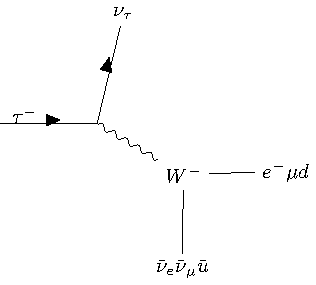
\includegraphics[width=0.35\textwidth]{"Figures/taudecay.pdf"}
    \caption{\label{fig:taudecay} diagram depicting the possible decays of the tau lepton: 65\% to a hadronic tau, 18\% to an electron, and 17\% to a muon (each with associated lepton neutrino)}
\end{center}
\end{figure} 
When the tau decays hadronically, many different intermediate mesons are produced. Each type of meson decay has a different signature, particularly when they hadronize and deposit their energy within HCAL. The Tau-POG has measured the central value systematic deviation as a form of scalar factor that is applied for an accurate result of measuring the tau's energy. This is split by the prongs (charged hadrons) and $\pi^0$ s.  

\begin{table}[h]
  \begin{center}
    \topcaption{Measured $\tauh$ energy scale correction for genuine $\tauh$'s across all years.}
    \label{tab:TES}
    \begin{tabular} { l | c  c  c }
      \hline \multicolumn{4}{c}{Correction (\%)} \\
      \hline Decay mode & 2016 & 2017 & 2018 \\ \hline
      $h^{\pm}$ & $-0.6$ & $0.7$ & $-1.3$  \\ 
      $h^{\pm}\pi^{0}$ & $-0.5$ & $-0.2$ & $-0.5$  \\ 
      $h^{\pm}h^{\pm}h^{\pm}$ & $0.0$ & $0.1$ & $-1.2$ \\ 
    \end{tabular}
  \end{center}
\end{table}

The deviation in the model is measured by taking the difference in data and MC for different values of hadronic tau energy. The uncertainty is measured for each decay mode considered in the analysis. Figures \ref{fig:taues} shows the differences in data and MC for the 1 prong + $\pi_0$ decay mode as a function of tau energy; all other tau decay modes are also measured. 

\begin{figure}[h!]
    \begin{center}
        \includegraphics[width=0.32\textwidth]{Figures/TauPOG/mtau_1ProngPi0_nominal_v3.pdf}
        \includegraphics[width=0.32\textwidth]{Figures/TauPOG/mtau_1ProngPi0_minus6percent_v3.pdf}
        \includegraphics[width=0.32\textwidth]{Figures/TauPOG/mtau_1ProngPi0_plus6percent_v3.pdf}
    \end{center}
    \caption{Tau mass distributions considering the nominal $\tau_h$ energy scale in simulation (left), or the $\tau_h$ energy scale shifted by -6 (left) or +6\% (right), in the $\mu\tau_h$ final state, for the 1 prong + $\pi^0$ decay mode.}
    \label{fig:taues}
\end{figure}

\subsection{$\tauh$ identification efficiency}

Genuine $\tauh$ identification efficiency can be different in Data and MC ~\cite{TAUIDTwiki}. To correct for this difference, measurements are 
made using genuine Z+jets production (Drell-Yan) to two $\tau$ leptons, one decays leptonically and the other hadronically. The invariant mass of the system is used as an observable. Naturally, this region has far more statistics than the control and signal regions in the pseudoscalar analysis. To measure the identification efficiency precisely, it is done in the inclusive event selection regions ~\ref{chap:selection} with an emphasis of simulation containing real taus. This measurement is done by the Tau POG, and the scale factors are provided to CMS. 
%For the $\mu\mu e \tauh$ and $\mu\mu\mu\tauh$ channels, scale factors are binned in 3 different $\pt$ bins: 30--35, 35--40, and 40+ \GeV. In the $\tauh\tauh$ final state, the efficiencies are also binned by decay mode. 

While used in the primary event and the parameter of interest in the fit, the efficiency's error is not considered in the overall systematic error as they are expected to have very little impact on fit and limits based on the 2016 result. 


\subsection{$e \rightarrow \tauh$  and $\mu \rightarrow \tauh$ misidentification rate}
The efficiency of the discriminators against electrons or muons misidentified as $\tauh$ candidates can also be different between simulation and data. 
These data/MC scale factors are
binned by barrel/endcap region of the measured $\eta(\tauh)$, and by $\tauh$ decay mode.
%Scale factors are measured to correct this difference and are applied to $e \rightarrow \tauh$ or $\mu \rightarrow \tauh$ in MC. 
Scale factors are measured to correct this difference misidentification and are applied to electrons or muons faking tau leptons in MC. 
Full information on misidentification measurements and application in analyses can be found in reference ~\cite{TAUIDTwiki}. 


The misidentification scale factors are derived by pass and fail regions. The regions are set up by selecting events where a reconstructed $\tauh$ passes the DNN working point and also fails the DNN discriminant against muons or electrons. The regions considered are QCD multijet, W+jets, and Z+jets---similar to the regions used in chapter \ref{chap:background}. QCD multijet is estimated from a same sign lepton region within data. W+Jets normalization is carefully selected from a region with high transverse mass. The visible mass distributions of the events in these regions are fit, and the overall signal yield remains constant in the pass and fail regions. 
The expected impact on the systematic error from these anti-lepton discriminators are expected to be very small so they are not included in the uncertainty model either.

%The scale factors are obtained by separating events with a reconstructed muon and a reconstructed $\tauh$ passing
%the deep tau ID into a category where the $\tauh$ passes or fails the discriminator against muons. All the processes in
%these regions are taken from simulation, except the QCD multijet background, which is estimated from SS data, and the W+jets background, which is normalized in a region with high $m_T$. The visible mass distributions in the pass and fail regions are fitted using the $e\to\tauh$ scale factor as parameter of interest. An increase of the POI causes an increase of the signal yield in the pass region and simultaneously a decrease of the signal in the fail region, such that the signal yield in the two regions combined is unchanged. 
%Additionally, the normalization of the $\PZ\to\Pe\Pe$ background is freely floating to modelna scale
%factor related to applying the discriminator against jets to muons. The scale factor applied to muons faking taus in the 
%analysis is the product of the scale factor of the discriminator against jets and scale factor of the discriminator against muons.


\subsection{Pileup re-weighting}

MC events are re-weighted using a minimum bias cross section equal to the luminosity for the corresponding year. This pileup re-weighting is to rescale the events for effective number of primary interactions during collisions. During Run II, pileup or the number of primary vertices in a crossing or underlying event could reach close to 100 and in Run III this will exceed 200.   

\subsection{Electron and muon identification efficiency}

Scale factors derived within the HTT group are applied for muons~\cite{SMHTTarXiv}, and the EGamma POG scale factors are applied for electrons~\cite{EGammaMVAID}. The scale factors for muons with $5<\pt<9$ GeV and $9<\pt<10$ GeV, are computed privately as there are no official numbers, and were approved by the MuonPOG in the 2016 analysis. These scale factors are used for the full RunII dataset. 
  
%\subsection{B tagging efficiency}

%The analysis vetoes events with at least one b tagged jet. The scale factors provided by the BTV POG~\cite{btvtwiki} are applied.

\subsection{Generator event weights and luminosity}

Generator weights are applied on an event-by-event basis. Samples produced with the aMCatNLO generator contain both positive and negative event weights. The presence of negative event weights reduces the effective yield of the samples and is included.
The event weights for simulation are scaled to the expected yields for each sample. 

To correct for differences between leading order and next to leading order cross sections, scale factors called K-factors are used. They are applied to W+Jets and Drell-Yan samples. For Drell-Yan a factor of 1.1637 is used and for W+Jets a factor of 1.221 is used.

\subsection{Low momentum muon selection}
Due to the selection of muons at 5 GeV, which is below the trigger threshold, scale factors were measured in the barrel and encaps using the tag and probe technique in the 2016 analysis. These factors are used to correct for low pt muon selection, in addition to the Muon POG's recommendation, to support correct simulation of data. 
\begin{table}[h!tbp]
\centering
\topcaption{Scale factors to correct for low momentum muon selection being less than the trigger threshold. 
\label{tab:event_yield}
}
\begin{tabular*}{0.6\textwidth}{c|c|c}
   & Barrel & Endcap \\\hline
Muons with $5 < pT < 9$ GeV & 0.956 & 0.930\\\hline
Muons with $9 < pT < 10$ GeV & 0.916 & 0.897\\\hline 
\end{tabular*}
\end{table}


\subsection{Visualizing the corrections}

The energy scales for the various leptons used in the analysis are not only changed in the nominal case, but their uncertainty is measured and then propagated to the fit model via changes in the normalization for the distribution. To visualize this and provide a cross check, distributions for the $\tau$, $\mu$, and $e$ energy scale shifts in the parameter of interest ( the mass of the di-muon system from the leading $\pt$ pseudoscalar $a$ particle) is plotted. 
These systematics for $\mu\mu\tau\tau$ channel are shown in figure \ref{fig:sys_shift_mmtt2016}.
\begin{figure}[ht!b]
  \centering
\includegraphics[width=0.31\textwidth]{Figures/outplots_v7plots_allsys_scale_m_etalt1p2Down/mll_fine_mmtt_inclusive.png} 
\includegraphics[width=0.31\textwidth]{Figures/outplots_v7plots_allsys_Nominal/mll_fine_mmtt_inclusive.png}
\includegraphics[width=0.31\textwidth]{Figures/outplots_v7plots_allsys_scale_m_etalt1p2Up/mll_fine_mmtt_inclusive.png} \\

    \caption{\label{fig:sys_shift_mmtt2016} Systematic Shift in the Uncertainty Model for 2016 $\mu\mu\tau\tau$ for the muon energy scale shift down (left), nominal (mid), and up (right), no data is shown on this plot as it directly reflects the signal region without the extraction cuts }
\end{figure}

In the end, the uncertainty considered in the fit model would then be the percent yield up and down as a flat error (log-normal) that affects the normalization of the template. Because the model is so statistically limited, the log-normal is sufficient in capturing the changes in the distributions over the fit range.  


\chapter{Event Selection}
\label{chap:selection}
%Selections.TeX
\section{Framing an Analysis at CERN}
In order to make a definitive statement and concrete hypothesis test, two perspectives are taken. 
There is the null hypothesis, ergo the hypothesis of the accepted standard within High Energy Physics --- the Standard Model --- which will comprise all possible events that are categorized as \textit{background}. 


Then the alternative hypothesis is taken to be the model that encompasses the Standard Model and adds additional physics that will contain events from the theory under consideration in the analysis \textit{signal}. For this analysis, it's events pertaining to the pseudoscalar Higgs-like particle "a", with two muons and two tau leptons in the final state. 

\section{Defining Signal and Control Regions}
The next thing to consider is what data should be used to test that hypothesis. Working with CMS, central Standard Model simulation samples are provided. Then to make the analysis competitive, regions of the full data and simulation are cut away in order to increase the number of signal events relative to background events. This process is known as "making cuts". In order to not bias the result, typically regions are setup to investigate the agreement of simulation with data (the control region) and to conduct the statistical hypothesis test (signal region). When the data and MC simulation agreement are reasonable in the control region then the statistical test can be made in the signal region.  



%Selections.TeX
\subsection{Optimizing Lepton Pair Selection}
\label{sec:selection}
In order to maximize the signal event yield - as it is expected that the analysis is statistically limited - a simple selection algorithm was used to identify good lepton pairs that come from the pseudo scalar $a$. Standard working point cuts are made, in addition to delta R cleaning, two prompt-like muons with opposite charge and leading scalar summed $P_t$ are chosen to form the first decay products of the $a$ and two opposite charged leading scalar summed $P_t$ $\tau$ leptons are chosen for the second $a$. This approach increased the signal acceptance compared to choosing mass window cuts to form the $a$ pairs. The following table reflects the pair matching efficiency study done with the preliminary dataset from 2016 NanoAODv6:
\begin{table}[h]
\begin{center}
    \topcaption{Lepton Pair Matching Efficiency}
    \label{tab:paireff}
\begin{tabular}{|c|c|c|c|c|c|c|c|c|c|c|}\hline
$a$ - Mass & 15     & 20    & 25    & 30    & 35    & 40    & 45    & 50    & 55    & 60 \\\hline
Efficiency & 0.87   & 0.82  &0.79   & 0.79  & 0.79  & 0.80  & 0.80  & 0.83  & 0.85  & 0.87 \\\hline 
\end{tabular}
\end{center}
\end{table}

All selections follow the Physics Object Group (POG) recommendations for object selection.
Since the search in 2016, a new identifier for $\tau$ leptons was considered using a Deep Neural Network (DNN) ~\cite{Hassanshahi:2797703}.
To identify the dimuon pair which come from one pseudoscalar $a$, several cuts were applied across all channels:
\begin{itemize}
    \item each $\mu_{pt} > 5.0$ GeV,
    \item charge $\text{dimuon} < 0$
    \item all $\mu_{iso}<=0.2$
    \item medium ID of the $\mu$, require global and track requirements (good $\mu$)
    \item number of b-quark tag jets $<$ 1 
    \item signal extraction cuts (not shown in data MC control plots)
    \begin{itemize}
    \item invariant mass of the 4 lepton system (AMass)$<120GeV$ 
    \item $M_{\mu\mu} > M_{\tau\tau}$   
    \end{itemize}
\end{itemize}


The trigger requirements are inclusive, selecting events that pass single muon and double muon triggers. Events that are triggered by the single muon triggers criteria contain muons that are isolated with either $22$, $24$, and $27$ GeV muons. Double muon triggers have a $17$ GeV threshold for the leading muon and $8$ GeV for the subleading muon. Triple muon triggers are used for the channels that have three muons in the final state and have a descending threshold of $12$, $10$, and $5$ GeV. These triggers and other minimal selection requirements are listed in table ~\ref{tab:inclusive_selection}.


\begin{table}[h!tbp]
\centering
\topcaption{Event selection requirements for the four decay channels. These demarcate cuts that are applied to the $\pt$, $\eta$, and isolation of the particle in addition to the trigger requirements. 
\label{tab:inclusive_selection}
}
\begin{tabular}{lllll}
  Channel     &  Trigger requirement                      & \multicolumn{3}{c}{Minimal lepton selection}                        \\ \cline{3-5}
              &                                            & $\pt$ ($\GeVns{}$)  & $\eta$                    &    Isolation      \\
\hline
$\mu\mu\tauh\tauh$  &  $\mu[22]$ $\mu[24]$  $\mu[27]$   or  $\mu\mu[17,8]$       &all $\pt^\mu>5$ $\pt^{\tauh}>18.5$    & $\abs{\eta^{\tauh}}<2.3$  &   Med. DNN $\tauh$   \\

$\mu\mu\mu\tauh$    &  $\mu[22]$ $\mu[24]$  $\mu[27]$   or  $\mu\mu[17,8]$                     & all $\pt^\mu>5$ $\pt^{\tauh}>18.5$      &  $\abs{\eta^\mu}<2.3$    &   $I^{\mu}<0.2$ \\

& or  $\mu\mu\mu[12,10,5]$  &  & & \\ 

$\mu\mu e \tauh$    &$\mu[22]$ $\mu[24]$  $\mu[27]$   or  $\mu\mu[17,8]$                         & all $\pt^\mu>5$ $\pt^e>7$      &  $\abs{\eta^e}<2.5$     &   $I^{e}<0.15$  \\
              &                          & $\pt^{\tauh}>18.5$    &  $\abs{\eta^{\tauh}}<2.4$ &   Med. DNN $\tauh$   \\

$\mu\mu e \mu $     & $\mu[22]$ $\mu[24]$  $\mu[27]$   or  $\mu\mu[17,8]$       &all $\pt^\mu>5$ $p_T^e >7\; p_T^\mu >5$      & $\abs{\eta^e}<2.4$      & $I^{e}<0.15$    \\
& or  $\mu\mu\mu[12,10,5]$  &  & & \\ 

\hline
\end{tabular}
\end{table}

%Muons are reconstructed and identified with requirements on the
%quality of the track reconstruction and on the number of hits in the tracker and muon systems. %~\cite{Chatrchyan:2012xi}.
%They are selected with $\pt>15\GeV$ and $\abs{\eta}<2.4$.

As mentioned in the instrumentation and detector section, the muon identification system uses the tracker to identify charged tracks and the muon chambers identify the particles later in their trajectory after they exit the solenoid. Typically "good" muons are those that are both associated with a track and their subsequent identification in the drift tubes or the CSC chambers. The average muon lifetime is 2.2 $\mu$s so they travel quite far from the interaction point the sub detectors.  The physics object group's recommendations are followed, which select muons with $\pt>15\GeV$ and $\abs{\eta}<2.4$ in addition to selecting only "good" muons.

%Electrons are reconstructed using tracks from the tracking system,
%calorimeter deposits in the ECAL, and a veto on objects with a large HCAL to
%ECAL energy. They are identified using a multivariate discriminant
%combining several quantities that describe the shape of the energy deposits
%in the ECAL, the quality of tracks, and the compatibility of the measurements from
%the tracker and the ECAL
%~\cite{Khachatryan:2015hwa}.


Electrons originating from the tau decay are reconstructed in by track association in tandem with energy deposition in the Electronic Calorimeter (ECAL). To clarify selection in the calorimeter systems, events are vetoed for candidate electrons that also show a substantial energy deposition in the HCAL. The hits and track quality from two separate algorithms, along with the geometrical and energy matching from the ECAL are used in a Multivariate Analysis (MVA) technique like Boosted Decision Trees (BDTs) to select good electrons for analysis 
~\cite{Khachatryan:2015hwa}.

%In order to reject leptons that originate from nonprompt interactions or are misidentified, a relative lepton
%isolation is defined and used:

Of critical importance in event selection is identification of unique particles, particularly differentiating between lepton candidates that come from the interaction vertex (prompt) and those that appear from decays down the line (nonprompt). Relative isolation is typically defined in order to ensure there is no overlap between candidate leptons. More details on this variable and it's usage in the Particle Flow algorithm can be found here  ~\cite{Sirunyan_2017}. 

\begin{equation}
I^{\ell} \equiv \frac{\sum_\text{charged}  \PT + \max\left( 0, \sum_\text{neutral}  \PT
                                         - \frac{1}{2} \sum_\text{charged, PU} \PT  \right )}{\PT^{\ell}}.
\label{eq:reconstruction_isolation}
\end{equation}
$\sum_\text{charged}  \PT$ is the scalar sum of the
transverse momenta of the charged particles originating from
the primary vertex and contained in a cone of size
$\Delta R = \sqrt{\smash[b]{(\Delta \eta)^2 + (\Delta \phi)^2}} = 0.4$\,(0.3)
centered on the muon (electron) direction. The sum $\sum_\text{neutral}  \PT$ is
a similar quantity for neutral particles.

%Concerning the Deep Neural Net for Tau identification, reconstruction of $\tauh$ candidates is performed with
%the hadrons-plus-strips (HPS) algorithm. The algorithm works by
%combining the signature of charged hadrons, tracks left in the tracker and
%energy deposits in the hadronic calorimeter, with the electron/photon
%signature of neutral pions reconstructed by collecting energy inside of
%``strips'' in $\eta-\phi$ space inside of the ECAL~\cite{Sirunyan:2018pgf}.
%The combination of these signatures provides the four-vector of the
%parent $\tauh$. Based on the overall neutral-versus-charged contents
%of the $\tauh$ reconstruction, a decay mode is assigned as either
%$h^{\pm}$, $h^{\pm}\pi^{0}$, $h^{\pm}h^{\mp}h^{\pm}$, or $h^{\pm}h^{\mp}h^{\pm}\pi^{0}$.
%The identification of $\tauh$ candidates makes use of isolation discriminators to reject quark
%and gluon jets misidentified as $\tauh$. The input variables to the DNN include variables
%related to the $\tauh$ isolation, $\tauh$ lifetime, and other detector-related
%variables. The threshold on the output discriminant depends on the $\tauh$ $\pt$ and provides
%a $\tauh$ ID and reconstruction efficiency of about 60\%.
%Two other DNNs are used to reject electrons and muons misidentified as $\tauh$ candidates using dedicated criteria
%based on the consistency between the measurements in the tracker, the calorimeters, and the muon detectors.
%Electrons are also selected using a Multivariate Analysis (MVA) technique, as recommended by the Electron POG.


To identify $\tauh$ candidates, the hadron-plus-strips (HPS) algorithm is used to identify the major modes of the hadronic tau decay ~\cite{Sirunyan_2018}. Typically events with hadronic prong are considered in combination with a number of neutral pions and missing transverse energy from the neutrinos. Pions almost always decay to photons, so an algorithm is considered that joins the identification of charged hadrons and neutral pions. 
The HPS algorithm combines inner track information, hits in the HCAL, and pion association in the ECAL by deposits in a $\eta,\phi$ strip region to identify hadronic tau leptons. 
The $\tauh$ is matched to $h^{\pm}$, $h^{\pm}\pi^{0}$, $h^{\pm}h^{\mp}h^{\pm}$, or $h^{\pm}h^{\mp}h^{\pm}\pi^{0}$ depending on the overall charge vs neutral constituents ~\cite{Sirunyan:2018pgf}.
In addition to HPS algorithms, a Deep Neural Network (DNN) was constructed to further aid in identification by discriminate between genuine tau leptons and those that originate from quark or gluon jets, electrons, or muons.  
In the DNN, the tau four-momentum and charge,
the number of charged and neutral particles used to reconstruct the tau candidate,
the isolation variables,
the compatibility of the leading tau track with coming from the primary vertex,
the properties of a secondary vertex in case of a multiprong tau decay,
observables related to the $\eta$ and $\phi$ distributions of energy reconstructed in the ECAL strips,
observables related to the compatibility of the tau candidate with being an electron, 
and the estimated pileup density in the event are all used. In total, 47 high-level input variables are incorporated 
~\cite{https://doi.org/10.48550/arxiv.2201.08458}.
In practice, the DNN has discriminators for muons, electrons, and jets that fake genuine taus and have efficiencies that go from 40\% to 90\% in a 10\% granularity of the discriminating variable. The medium working point is used for each of these discriminators. 


%\begin{figure}[ht!b]
%  \centering
%  \includegraphics[width=0.47\textwidth]{Figures/outplots_2016_combo_mmmt_Nominal/AMass_blinded_mmmt_inclusive.png}
%  \includegraphics[width=0.47\textwidth]{Figures/outplots_2016_combo_mmet_Nominal/AMass_blinded_mmet_inclusive.png}\\
%  \includegraphics[width=0.47\textwidth]{Figures/outplots_2016_combo_mmem_Nominal/AMass_blinded_mmem_inclusive.png}
%  \includegraphics[width=0.47\textwidth]{Figures/outplots_2016_combo_mmtt_Nominal/AMass_blinded_mmtt_inclusive.png}\\
%    \caption{\label{fig:AMass_2016_v1} Invariant Mass of the four lepton system for 2016 data in all Channels}
%\end{figure}
%\begin{figure}[ht!b]
%  \centering
%  \includegraphics[width=0.47\textwidth]{Figures/outplots_2017_combo_mmmt_Nominal/AMass_blinded_mmmt_inclusive.png}
%  \includegraphics[width=0.47\textwidth]{Figures/outplots_2017_combo_mmet_Nominal/AMass_blinded_mmet_inclusive.png}\\
%  \includegraphics[width=0.47\textwidth]{Figures/outplots_2017_combo_mmem_Nominal/AMass_blinded_mmem_inclusive.png}
%  \includegraphics[width=0.47\textwidth]{Figures/outplots_2017_combo_mmtt_Nominal/AMass_blinded_mmtt_inclusive.png}\\
%    \caption{\label{fig:AMass_2017_v1} Invariant Mass of the four lepton system for 2017 data in all Channels}
%\end{figure}
%\begin{figure}[ht!b]
%  \centering
%  \includegraphics[width=0.47\textwidth]{Figures/outplots_2018_combo_mmmt_Nominal/AMass_blinded_mmmt_inclusive.png}
%  \includegraphics[width=0.47\textwidth]{Figures/outplots_2018_combo_mmet_Nominal/AMass_blinded_mmet_inclusive.png}\\
%  \includegraphics[width=0.47\textwidth]{Figures/outplots_2018_combo_mmem_Nominal/AMass_blinded_mmem_inclusive.png}
%  \includegraphics[width=0.47\textwidth]{Figures/outplots_2018_combo_mmtt_Nominal/AMass_blinded_mmtt_inclusive.png}\\
%    \caption{\label{fig:AMass_2018_v1} Invariant Mass of the four lepton system for 2018 data in all Channels}
%\end{figure}

\begin{figure}[ht!b]
  \centering
  \includegraphics[width=0.47\textwidth]{Figures/outplots_mmmt_combo_Nominal/AMass_blinded_combined.png}
  \includegraphics[width=0.47\textwidth]{Figures/outplots_mmet_combo_Nominal/AMass_blinded_combined.png}\\
  \includegraphics[width=0.47\textwidth]{Figures/outplots_mmem_combo_Nominal/AMass_blinded_combined.png}
  \includegraphics[width=0.47\textwidth]{Figures/outplots_mmtt_combo_Nominal/AMass_blinded_combined.png}\\
    \caption{\label{fig:AMass_v1} Invariant mass of the four lepton system for 2018 data in all Channels}
\end{figure}

\begin{figure}[ht!b]
  \centering
  \includegraphics[width=0.47\textwidth]{Figures/outplots_allyears_combo_Nominal/AMass_blinded_combined.png}
  \includegraphics[width=0.47\textwidth]{Figures/outplots_allyears_combo_Nominal/pt_1_combined.png}\\
  \includegraphics[width=0.47\textwidth]{Figures/outplots_allyears_combo_Nominal/eta_1_combined.png}
  \includegraphics[width=0.47\textwidth]{Figures/outplots_allyears_combo_Nominal/pt_3_combined.png}\\
    \caption{\label{fig:AMass_RunII}  Several data-MC control plots for full RunII data in all Channels}
\end{figure}






\chapter{Background Estimation}
\label{chap:background}
%background.TeX

Due to the stringent cuts in the tight signal region and absense of resonance, MC simulation suffers from low statistics for some background processes.  
Therefore, in addition to the MC simulation, a data driven method is used to estimate a significant portion of background that is not reliably estimated using MC.

The hadronic $\tau$ decays produce jets; therefore, jets coming from other processeses effectively fake the hadronic $\tau$ signature. This is a non-trival fake rate that needs to be measured and accounted for in this analysis. 

In order to conduct the data driven method, a proportion is made to extract the jet faking tau background. Generally, this proportion is constructed using a region orthogonal to the statistical hypothesis test. For example, one requirement could be a charge sign inversion on a lepton pair used in the final state. In this orthogonal region and in the tight signal region, tight and loose identification criteria are made to extrapolate the scale factor that estimates the tau's fake rate. 
The tight identification should be excellent at selecting genuine tau leptons and the loose identification more inclusive to all tau leptons, even those that are fake. 
Therefore, using the orthogonal reigons---same sign and opposite sign---along with the loose signal region, one can extrapolate the number of events in the tight signal region. Due to the four regions, the method is also referred to as the ``ABCD" method. 


\section{Brief outline of the fake rate method}
The fake rate function in the same sign (SS) region is \textit{known}.
Events passing loose identification---that includes tight indentification---in the opposite sign (OS) region is \textit{known}.
Events passing in the tight signal region is \textit{unknown}. 
Assuming that the loose and tight identification is not dependent on the sign of the leptons. Then one can make the equivalence statement: 
\begin{equation}
\label{eq:abcd}
\frac{\text{Events}_\text{SS Tight}}{\text{Events}_\text{SS Loose}} \doteq \frac{\text{Events}_\text{OS Tight}}{\text{Events}_\text{OS Loose}}
\text{.}
\end{equation}
To make the expression more precise, the fake rate function is typically parametrized in lepton candidate transverse momentum. 
 Also, prompt MC is subtracted from data, which is motivated by estimating the true jet faking tau background (non-prompt taus). If tau leptons in MC are identified as prompt then it is unlikely that the tau is a jet, so they are removed: 
\begin{equation}
f(p_T)=\frac{\text{Data Events}_\text{S.S. Tight} - \text{Prompt MC Background}_\text{S.S. Tight}}{{\text{Data Events}_\text{S.S. Loose} - \text{Prompt MC Background}_\text{S.S. Loose}}}
\text{.}
\end{equation} 

After the measurement is made for each tau candidate, the fake rate is applied as an event weight---$w(f(p_T))$ a transfer function explained~\ref{eq:frw}---to the opposite sign loose region in order to extrapolate to the tight signal region. So isolating the events in the tight signal region and flipping the relation in equation \ref{eq:abcd}, one obtains the result: 
\begin{equation}
\text{Events}_\text{OS Tight} = w(f(p_T))\cdot \text{Events}_\text{OS Loose} \;\text{.}
\end{equation}

\section{Measurement of the fake rate}
To measure the fake rate, multiple categories are considered and motivated through the processes which produce jets. As outlined in the SM Higgs decays to tau leptons analysis and its supporting document on fake rate measurements, several regions are used to determine the fake rate ~\cite{SMHTTarXiv}. The separate jet ``enriched" background processes are used for each final state
\begin{itemize}
	\item QCD multijet targeting the majority of jet→ \tauh fake events in the $\mu\mu\tau\tau$ final state,
	\item W+jets targeting jets mostly in the $\mu\mu e\tau$ and $\mu\mu\mu\tau$ final states,
	\item \ttbar events targeting fully-hadronic or semi-leptonic decays.
\end{itemize} 



The fake rates are then measured as a function of $p_T$ of the object and for final states involving hadronic tau leptons, and are further split into subcategories depending on the decay mode.  
W+jets with no jets and one jet, QCD multi-jet with no jets, one jet, and more jets, and $t\bar{t}$ inclusive jets make up the total number of background categories that are measured. 
At high hadronic tau $p_T$ (greater than 100\GeV), negative fake rates are possible because of low statistics and the linear fit model extrapolation, so if the candidate tau has a $p_T$ of greater than 100\GeV the rate at 100\GeV is applied. 
In order to combine the fake rates from these ``enriched'' background processes and use it in an ABCD approach, the fraction of events for each of the background process are combined in an overall fake rate that is still parametrized by $\pt$ and category.  

%In the QCD multijet region, there is no way to estimate it with pure MC simulation. Therefore, in order to estimate the QCD contribution all MC simulation events are subtracted before the measurements. Then the remaining fake rate measurement in the determination region is assumed to be from QCD.

%In the W+Jets region, similarly all MC is subtracted except for the W+Jets simulation. Note that QCD contamination is minimal because of the dominance of the W boson resonance. 

%In the $t\bar{t}$ region it is the same as the W+Jets regions, except the subtraction is $t\bar{t}$; however, there is also an isolation region that is used because the fake rate for this process is expected to be very small and actually calculable using MC, so in addition to the genuine $t\bar{t}$ events, the fraction of jets faking hadronic taus are also included in the subtraction. 


%For more information on the specfic events that are targeted in the QCD multijet, W+Jets, and $t\bar{t}$ regions the SM reference has all the categories with a detailed description of the subtraction  

Therefore the following steps are done for each final state to measure the fake rate:
\begin{enumerate}
\item[1.] Determine fake rate scale factor parametrized in candidate lepton $\pt$ in the QCD, W+jets, and $t\bar{t}$ regions
\item[2.] Make corrections based on the other lepton in the channel for closure 
\item[3.] Make corrections based on the differences between the first step and the signal region
\item[4.] Determine the fraction of QCD, W+jets, and $t\bar{t}$ events in the signal region.
\end{enumerate} 

To help in the understanding of the measurement regions, a table listing the enriched background and targeted final state along with the cuts and the anti-isolation requirement (the non-orthogonal condition in the ABCD method) will be presented. 
As indicated in the tables below, $\mu\tau$ and $ e \tau$ measured states share the same categories. For the $\tau\tau$ state, only the QCD ``enriched'' background category is considered. 
For the $\mu\mu e\mu$ final state in the application, the fake rate measurements from the $\mu\tau$ and $e \tau$ measured states are used for the corresponding lepton ($\mu or e$). 


\begin{table}[h!tbp]
\centering
\topcaption{Jet ``enriched'' background categories with cuts for each measured state, $\mu\tau$ and $e \tau $ have the same so they will be combined with the assumption that $l$ demarcates the muon or electron. Baseline selection cuts for events are made by default as listed in section~\ref{chap:selection} without the signal extraction cuts. 
\label{tab:ffmeasure}
}
\begin{tabular}{|c|c|p{0.3\textwidth}|p{0.3\textwidth}|}
\hline
background &  measured state      &  cuts & anti-isolation \\\hline 

QCD & $\mu\tau$/$ e\tau$  & SS leptons Isolation \hspace{.1\linewidth} $l$ $\in(0.02,0.15)$ & $\tau$ VVVLoose DNN but fails Med. DNN \\
    & $\tau\tau$  & SS leptons subleading $\tau$ pass Med. DNN and leading VVVLoose DNN & leading $\tau$ fails Med DNN \\\hline

W+Jets & $\mu\tau$/$ e\tau$  & SS leptons $m_T$ between $l$ and $p_T^{\text{miss}}$ $> 70 $ GeV & $\tau$ VVVLoose DNN but fails Med. DNN \\\hline

$t\bar{t}$ & $\mu\tau$/$ e\tau$  & SS leptons number of b-tag jets $\geq 1 $ & $\tau$ VVVLoose DNN but fails Med. DNN \\\hline
\end{tabular}
\end{table}
Fake factor measurements for the $\mu\tau$ measured state in the QCD region for 2017 is included in figure \ref{fig:fit_raw_mt_0jet_qcd}. 
Only plots pertaining to the $ e \tau$ and $ \mu \tau$ states were created, but all states measured. 
The rest of the measurements are included in Appendix \ref{app:ffmeas}. For a more detailed description of the data driven background method along with the measurements for the closure and extra correction terms regard reference~\cite{AN16355}.




\begin{figure}[ht!b]
\centering
%\includegraphics[width=0.31\textwidth]{Figures/FF/plots_mt_2016/fit_rawFF_mt_qcd_0jet.pdf}
\includegraphics[width=0.85\textwidth]{Figures/FF/plots_mt_2017/fit_rawFF_mt_qcd_0jet.pdf}\\
%\includegraphics[width=0.31\textwidth]{Figures/FF/plots_mt_2018/fit_rawFF_mt_qcd_0jet.pdf}\\
\caption{\label{fig:fit_raw_mt_0jet_qcd} Fake factors determined in the QCD multijet determination region with 0 jets in the $\mu\tau$ measured state in 2017. They are fitted with linear functions as a function of the $\tauh$ $\pt$. The green and purple lines indicate the shape systematics obtained by uncorrelating the uncertainties in the two fit parameters returned by the fit.  }
\end{figure}





\clearpage

\section{Application of the fake rate method}

After the jet faking tau rate is measured, it is then applied to events that are identified as loose and not tight. Since the final state involves two tau leptons, this procedure is applied to each tau lepton in the final state, thus requiring application of the fake rate in three different scenarios. The final weight is then applied depending on the pass and fail criteria of each lepton candidate. In the scenario where the event fails both candidate requirements, then a minus sign is included, to avoid the case of double counting.  
 The weight is effectively a transfer factor that is created using the fake rate measured earlier. The transfer factor has its form because the weight is the ratio of tight to loose---tight excluded---instead of tight to loose---tight included. 
\begin{itemize}
\item{If event fails identification for $\tau$ 1:\begin{equation}\label{eq:frw} w_1(p_T)=\frac{f_{1}(p_T)}{1-f_{1}(p_T)}\end{equation}}
\item{If event fails identification for $\tau$ 2:\begin{equation}w_2(p_T)=\frac{f_{2}(p_T)}{1-f_{2}(p_T)}\end{equation}}
\item{If event fails identification for both:\begin{equation}w_{12}(p_T)=-\frac{f_{1}(p_T)}{1-f_{1}(p_T)}\cdot\frac{f_{2}(p_T)}{1-f_{2}(p_T)}\end{equation}}
\end{itemize}

To illustrate the different regions in the ABCD method along with each tau candidate, a diagram was drawn depicting the scenarios and is shown in figure \ref{fig:fakefactor_reg}. 
\begin{figure}[ht!b]
\label{fig:fakefactor_reg}
  \includegraphics[width=0.9\textwidth]{"Figures/fakefactor_diagram.pdf"}
    \caption{ ABCD method diagram depicting the measurement and application regions for each \tauh lepton in the final sate.}
\end{figure}

This fake factor methodology has been used by other analyses such as the SM Higgs measurement with an associated Z boson ~\cite{CMS-PAS-HIG-19-010} . 

For a closure test, the same criteria are applied to the selection of the tight same sign region. The vast majority of the background should be jets faking taus in that case. Indeed it is shown in figure \ref{fig:fakefactor_validation}.
  
\begin{figure}[ht!b]
  \includegraphics[width=0.65\textwidth]{"Figures/outplots_2016_smFF_mmmt_Nominal/AMass_blinded_mmmt_FF_SS_validation.png"}
    \caption{\label{fig:fakefactor_validation} Validation of the fake factor method. Fake factors are applied to the same sign tight region.}
\end{figure}


\chapter{Control Plots}
\label{chap:plots}
\input{chapters/Controlplots.tex}

\chapter{Statistical Inference Modeling}
\label{chap:stat}
%fit Models
\section{Statistical Inference at CERN}
In order to conduct a hypothesis test, a test statistic is needed. This is constructed through the \textit{profile likelihood ratio} and then a confidence level is set using the test statistic ~\cite{Cowan_2011}.
So construction of a likelihood is required, the test statistic from the likelihood, and a way to calculate a confidence level to complete the hypothesis test.
To construct the likelihood, the typical approach is to assume a Poisson distribution for the events in the $i-th$ bin and then "smear" it by multiplying it with a Gaussian that is also dependent on the events. The events are split, into signal and background. Because an alternative hypothesis is explored and a-priori the amount of signal events isn't known, it is floated by a coefficient denoted as $\mu$ - the signal strength. For an upper limit this value is changed until the cumulative distribution function of the likelihood reaches the desired confidence or p-value.  

\[\mathcal{L}(\text{data}|\mu,\theta) = \text{Poisson}(\text{data},\mu\cdot s(\theta)+b(\theta)) \cdot p(\tilde{\theta}|\theta) \]
For binned $n_i$ events in bin label $i$:
\begin{equation}Poisson(\text{data},\mu\cdot s(\theta)+b(\theta)) = \prod_i \frac{(\mu s_i+b_i)^n}{n_i !}e^{-\mu s_i -b_i}
\end{equation}

In the case of the pseudoscalar analysis discussed in this paper a slightly different likelihood is considered. A shape-based approach is considered, which instead of a product of many simple Poisson probability density functions, probability distribution functions are used over the entirety of the fit variable (or parameter of interest POI). Multiple PDFs can be combined in this scenario, but the important difference is the absence of any binning. Therefore a good fit is required to have a good description of the events.  

Unbinned or Parametric likelihood functions over $k$ events, $S$ and $B$ the total event rate, $f_s(x_i)$ and $f_b(x_i)$ the \textit{pdfs}
 \[Poisson(\text{data},\mu\cdot s(\theta)+b(\theta)) = k^-1 \prod_i(\mu S f_s(x_i) + B f_b(x_i))e^{-\mu S - B}\]

Specifically for the pseudoscalar analysis, a product of Bernstein polynomials for $f_b(x_i)$ and Voigtian functions for $f_s(x_i)$ are used. The Bernstein captures the slow changing background that is basically constant in a 2GeV mass window and the Voigtian captures the sharp peaking dimuon mass signal. Details in the analysis will be saved for after the overview of the stat inference model. 

To outline the typical approach in the profile likelihood method, the follow steps are done in an effort to set the limit
\begin{enumerate}
\item {To form the test statistic, the \textit{profile likelihood ratio} is used 
  \[\tilde{q}_\mu = -2 \ln \frac{\mathcal{L}(\text{data}|\mu,\hat{\hat{\theta}}_\mu)}{\mathcal{L}_\text{max}(\text{data}|\hat{\mu},\hat{\theta})} \;\; 0\leq \hat{\mu} \leq \mu \]
  Where $\hat{\mu}$ and $\hat{\theta}$ are the maximum likelihood estimators. 
  }
  \item Find the \textit{observed} value of the test statistic $\tilde{q}_\mu^{obs}$ for given signal strength $\mu$.
  \item Find values of the nuisance parameters that best describe the experimentally observed data by maximizing the likelihood.
  \item Generate toy MC pseudo data to construct probability density functions for signal and background $f(\tilde{q}_\mu|\mu,\hat{\theta}_\mu)$ and $f(\tilde{q}_\mu|0,\hat{\theta}_\mu)$ for background only hypothesis. These pdfs are the pdfs of the test statistic under the assumption of a signal strength.
  \item Generate toy MC pseudo data to construct probability density functions for signal and background $f(\tilde{q}_\mu|\mu,\hat{\theta}_\mu)$ and $f(\tilde{q}_\mu|0,\hat{\theta}_\mu)$ for background only hypothesis.
  \item {Define p-values to be associated with the actual observation for both s+b and b only hypotheses
  \[ p_\mu = P(\tilde{q}_\mu \ge \tilde{q}_\mu^{obs}| s+b) = \int_{\tilde{q}_\mu^{obs}}^\infty f(\tilde{q}_\mu |\mu,\hat{\theta}_\mu^{obs} ) d\tilde{q}_\mu\]
  \[ 1- p_b = P(\tilde{q}_\mu \ge \tilde{q}_b^{obs}| b) = \int_{\tilde{q}_b^{obs}}^\infty f(\tilde{q}_\mu |\mu,\hat{\theta}_b^{obs} ) d\tilde{q}_\mu\]
   Then take the ratio to form the confidence levels
  \[ CL_s (\mu)  = \frac{p_\mu}{1-p_b}\]
  }
  \item{ Let $\alpha$ be the measure of confidence, then for $\mu=1$ if $CL_s \leq \alpha$ then the signal hypothesis is rejected in favor of the background only hypothesis}
  \item {Further to quote the $95\%$ confidence level on $\mu$, we need to adjust the signal strength ($\mu$) , until $CL_s = 0.05$}
\end{enumerate}


\section{Worked Example for Low Stat Analyses}
Order of magnitude estimates for low stat analyses like the Higgs decay to pseudoscalars can be obtained by considering a very simple statistical inference model. 

Suppose there are $N$ events 
\begin{equation}
\label{eq:Nevents}
N = B\cdot \sigma \cdot A\cdot \mathcal{L}
\end{equation}
where $B$ is the branching fraction for the physics process, $A$ is the signal acceptance, $\sigma$ is the cross section, and $\mathcal{L}$ is the luminosity.

Thus given a model that has the dependent variables, the upper 95\% limit on the branching fraction can be found. 

In general \ref{eq:Nevents} works; however, a likelihood model is needed to fully get the estimate of the number of events expected. 

As outlined in binned-likelihood models in CMS ~\cite{Cowan_2011}, suppose that the number of expected events follows a Poisson distribution. Then in that case if the background model would predict 0 average events, then the upper 95\% bound in that case is 3.7 events. 

Inverting the relation
\[B = \frac{N}{\sigma \cdot A\cdot \mathcal{L}}\]
Selecting the signal acceptance from the pseudoscalar analysis (2016 $\mu\mu\mu\tau$) 
\[ A = \frac{\text{events pass all cuts}}{\text{starting events}} = \frac{1293}{250000} \approx 0.005 \]
and taking the cross section of the gluon gluon fusion for the parent particle in the decay chain $\sigma = 48 \text{pb}$ along with the luminosity for 2016 $\mathcal{L} = 35,900 \text{pb}^{-1}$

Then the upper 95\% limit on the branching fraction is 

\[B =  \frac{N}{\sigma \cdot A\cdot \mathcal{L}} = 0.00043 = 4.3 \times 10^{-4}\]



\section{Fit model for pseudoscalar Higgs search}
After the signal extraction cuts are applied, an unbinned parametric likelihood fit was done with various shapes depending on the background and signal categorization. There is one signal distribution depending on the hypothesized $a$ mass, and two background distributions that are considered in the final fit. The two contributing background distributions originate from "Irreducible" events coming from two Z bosons (ZZ) and from "Reducible" events coming from jets faking tau leptons (FF).  

%%For the signal, a Voigtian function is used to fit the $a$ mass spectrum in a small window - 2GeV - of the hypothesized $a$ mass for the sample \ref{fig:fit_sig}. The Voigtian shape was chosen to reflect the narrow simulated peak that is statistically smeared by experimental measurement.

For the signal, a Voigtian function is used to fit the pseudoscalar $a$ mass spectrum in a small window - 2GeV - of the hypothesized $a$ mass for the sample as in figure \ref{fig:fit_sig}. The Voigtian shape was chosen to reflect the narrow simulated peak that is statistically smeared by experimental measurement. The Voigtian shape has one extra degree of freedom compared to the Gaussian. This parameter controls the Lorentzian factor in the Voigtian. For the signal MC the distributions tend to increase in standard deviation as the mass approaches 60 GeV. To compare the signal MC distributions, they are all plotted in figure \ref{fig:fit_sig_all}.


\begin{figure}[ht!b]
    \centering 
    \includegraphics[width=0.47\textwidth]{Figures/DiMuonMass_combined_sig.pdf}
    \caption{\label{fig:fit_sig_all} Signal fit using a Voigtian function}
\end{figure}
%\begin{figure}[ht!b]
%  \centering
%  \includegraphics[width=0.47\textwidth]{Figures/Fits_Dec2020/DiMuonMass_sig_mmet.pdf}
%  \includegraphics[width=0.47\textwidth]{Figures/Fits_Dec2020/DiMuonMass_sig_mmmt.pdf}\\
%  \includegraphics[width=0.47\textwidth]{Figures/Fits_Dec2020/DiMuonMass_sig_mmtt.pdf}
%  \includegraphics[width=0.47\textwidth]{Figures/Fits_Dec2020/DiMuonMass_sig_mmem.pdf}\\
%    \caption{\label{fig:fit_sig} Signal fit using a Voigtian function}
%\end{figure}
\begin{figure}[ht!b]
  \centering
  \includegraphics[width=0.47\textwidth]{Figures/2016_mmmt_combination/40_Nominal_a40_2016_mmmt_Nominal.png}
  \includegraphics[width=0.47\textwidth]{Figures/2016_mmet_combination/40_Nominal_a40_2016_mmet_Nominal.png}\\
  \includegraphics[width=0.47\textwidth]{Figures/2016_mmtt_combination/40_Nominal_a40_2016_mmtt_Nominal.png}
  \includegraphics[width=0.47\textwidth]{Figures/2016_mmem_combination/40_Nominal_a40_2016_mmem_Nominal.png}\\
    \caption{\label{fig:fit_sig} Signal fits using a voiigtian function for a-mass at 40GeV }
\end{figure}

In order to obtain precise signal resolution, shapes from the signal samples in intervals of 5 GeV accross the whole fit range 20-60 GeV are interpolated using spline functions. Thus precise limits can be obtained at the 1 GeV granularity. Predicated upon the fit model, using the spline in a refit would produce reults that are close to the original fit to signal ensuring that in the statistical inference model that the signal is well modeled for all mass points. A spline function is necessary for each degree of freedom in the model. An example of such functions are shown in figure \ref{fig:spline_2016_mmmt}. The bands that envelope the spline indicate the spread and the accepted error on the spline in the statistical inference model, more details are discussed in the systematics section.  
\begin{figure}[ht!b]
    \centering 
    \includegraphics[width=0.47\textwidth]{Figures/2016_mmmt_combination/DiMuonMass_AlphaConstraint_2016_mmmt.pdf}
    \includegraphics[width=0.47\textwidth]{Figures/2016_mmmt_combination/DiMuonMass_SigmaConstraint_2016_mmmt.pdf}\\
    \includegraphics[width=0.47\textwidth]{Figures/2016_mmmt_combination/DiMuonMass_MeanConstraint_2016_mmmt.pdf}
    \includegraphics[width=0.47\textwidth]{Figures/2016_mmmt_combination/DiMuonMass_NormConstraint_2016_mmmt.pdf}\\
    \caption{\label{fig:spline_2016_mmmt} spline functions for 2016 mmmt 3rd order used for Alpha, Sigma, and Normalization, linear fit for the Mean}
\end{figure}
\begin{figure}[ht!b]
    \centering 
    \includegraphics[width=0.47\textwidth]{Figures/2016_mmet_combination/DiMuonMass_AlphaConstraint_2016_mmet.pdf}
    \includegraphics[width=0.47\textwidth]{Figures/2016_mmet_combination/DiMuonMass_SigmaConstraint_2016_mmet.pdf}\\
    \includegraphics[width=0.47\textwidth]{Figures/2016_mmet_combination/DiMuonMass_MeanConstraint_2016_mmet.pdf}
    \includegraphics[width=0.47\textwidth]{Figures/2016_mmet_combination/DiMuonMass_NormConstraint_2016_mmet.pdf}\\
    \caption{\label{fig:spline_2016_mmet} spline functions for 2016 mmet 3rd order used for Alpha, Sigma, and Normalization, linear fit for the Mean}
\end{figure}
\begin{figure}[ht!b]
    \centering 
    \includegraphics[width=0.47\textwidth]{Figures/2016_mmtt_combination/DiMuonMass_AlphaConstraint_2016_mmtt.pdf}
    \includegraphics[width=0.47\textwidth]{Figures/2016_mmtt_combination/DiMuonMass_SigmaConstraint_2016_mmtt.pdf}\\
    \includegraphics[width=0.47\textwidth]{Figures/2016_mmtt_combination/DiMuonMass_MeanConstraint_2016_mmtt.pdf}
    \includegraphics[width=0.47\textwidth]{Figures/2016_mmtt_combination/DiMuonMass_NormConstraint_2016_mmtt.pdf}\\
    \caption{\label{fig:spline_2016_mmtt} spline functions for 2016 mmtt 3rd order used for Alpha, Sigma, and Normalization, linear fit for the Mean}
\end{figure}
\begin{figure}[ht!b]
    \centering 
    \includegraphics[width=0.47\textwidth]{Figures/2016_mmem_combination/DiMuonMass_AlphaConstraint_2016_mmem.pdf}
    \includegraphics[width=0.47\textwidth]{Figures/2016_mmem_combination/DiMuonMass_SigmaConstraint_2016_mmem.pdf}\\
    \includegraphics[width=0.47\textwidth]{Figures/2016_mmem_combination/DiMuonMass_MeanConstraint_2016_mmem.pdf}
    \includegraphics[width=0.47\textwidth]{Figures/2016_mmem_combination/DiMuonMass_NormConstraint_2016_mmem.pdf}\\
    \caption{\label{fig:spline_2016_mmem} spline functions for 2016 mmem 3rd order used for Alpha, Sigma, and Normalization, linear fit for the Mean}
\end{figure}

For the irreducible background coming from $ZZ\rightarrow 4 l$, a Bernstein polynomial is used to fit the shape over the entire $a$ mass range in figure \ref{fig:fit_ZZ}. Depending on the final state and shape the degree is chosen to reflect accurate errors in the model. A Fischer F-test was conducted and there doesn't seem to be enough statistics in the bins to provide an accurate difference in the log-likelihood in order to recommend a leading degree. Thus for $\mu\mu\tau\tau$ and $\mu\mu e \tau$, a linear fit is used. For the channels that do have more events like $\mu\mu\mu\tau$ and $\mu\mu e \mu$ - albeit even for a lower number of integrated events - a parabolic order is used. Plotted error bands reflect a simulation of 315 events in a RooFit simulation and is only meant to visualize possible 1 sigma differences in the shape. The true value of the error estimation on the parameters are take from the fit itself and can be seen in the plots, and are later shown in the impacts which demonstrate how the fit parameters effect the overall statistical inference model \ref{fig:impacts_2016_mmmt}. 

%\begin{figure}[ht!b]
%  \centering
%  \includegraphics[width=0.47\textwidth]{Figures/Fits_Dec2020/DiMuonMass_ZZ_mmet.pdf}
%  \includegraphics[width=0.47\textwidth]{Figures/Fits_Dec2020/DiMuonMass_ZZ_mmmt.pdf}\\
%  \includegraphics[width=0.47\textwidth]{Figures/Fits_Dec2020/DiMuonMass_ZZ_mmtt.pdf}
%  \includegraphics[width=0.47\textwidth]{Figures/Fits_Dec2020/DiMuonMass_ZZ_mmem.pdf}\\
%    \caption{\label{fig:fit_ZZ} irreducible background fit using 4th degree Bernstein polynomial}
%\end{figure}
\begin{figure}[ht!b]
  \centering
  \includegraphics[width=0.47\textwidth]{Figures/2016_mmmt_combination/2_Nominal_irBkg_2016_mmmt_Nominal.png}
  \includegraphics[width=0.47\textwidth]{Figures/2016_mmet_combination/1_Nominal_irBkg_2016_mmet_Nominal.png}\\
  \includegraphics[width=0.47\textwidth]{Figures/2016_mmtt_combination/1_Nominal_irBkg_2016_mmtt_Nominal.png}
  \includegraphics[width=0.47\textwidth]{Figures/2016_mmem_combination/2_Nominal_irBkg_2016_mmem_Nominal.png}\\
    \caption{\label{fig:fit_ZZ} irreducible background fit using Bernstein polynomials}
\end{figure}

For the jet faking tau background, a Bernstein polynomial is also used to fit the shape over the entire $a$ mass range in figure \ref{fig:fit_FF}. As with the ZZ - irreducible background - the jet faking tau background polynomial degree is chosen to reflect accurate errors in the model. 


%\begin{figure}[ht!b]
%  \centering
%  \includegraphics[width=0.47\textwidth]{Figures/Fits_Dec2020/DiMuonMass_FF_mmet.pdf}
%  \includegraphics[width=0.47\textwidth]{Figures/Fits_Dec2020/DiMuonMass_FF_mmmt.pdf}\\
%  \includegraphics[width=0.47\textwidth]{Figures/Fits_Dec2020/DiMuonMass_FF_mmtt.pdf}
%  \includegraphics[width=0.47\textwidth]{Figures/Fits_Dec2020/DiMuonMass_FF_mmem.pdf}\\
%    \caption{\label{fig:fit_FF} irreducible background fit using 4th degree Bernstein polynomial}
%\end{figure}

\begin{figure}[ht!b]
  \centering
  \includegraphics[width=0.47\textwidth]{Figures/2016_mmmt_combination/2_Nominal_Bkg_2016_mmmt_Nominal.png}
  \includegraphics[width=0.47\textwidth]{Figures/2016_mmet_combination/1_Nominal_Bkg_2016_mmet_Nominal.png}\\
  \includegraphics[width=0.47\textwidth]{Figures/2016_mmtt_combination/1_Nominal_Bkg_2016_mmtt_Nominal.png}
  \includegraphics[width=0.47\textwidth]{Figures/2016_mmem_combination/2_Nominal_Bkg_2016_mmem_Nominal.png}\\
    \caption{\label{fig:fit_FF} reducible background fit using Bernstein polynomials}
\end{figure}

The rest of the channels and years are shown below. 

\begin{figure}[ht!b]
  \centering
  \includegraphics[width=0.47\textwidth]{Figures/2017_mmmt_combination/40_Nominal_a40_2017_mmmt_Nominal.png}
  \includegraphics[width=0.47\textwidth]{Figures/2017_mmet_combination/40_Nominal_a40_2017_mmet_Nominal.png}\\
  \includegraphics[width=0.47\textwidth]{Figures/2017_mmtt_combination/40_Nominal_a40_2017_mmtt_Nominal.png}
  \includegraphics[width=0.47\textwidth]{Figures/2017_mmem_combination/40_Nominal_a40_2017_mmem_Nominal.png}\\
    \caption{\label{fig:2017_fit_sig} 2017 Signal fit using a Voigtian function}
\end{figure}

\begin{figure}[ht!b]
    \centering 
    \includegraphics[width=0.47\textwidth]{Figures/2017_mmmt_combination/DiMuonMass_AlphaConstraint_2017_mmmt.pdf}
    \includegraphics[width=0.47\textwidth]{Figures/2017_mmmt_combination/DiMuonMass_SigmaConstraint_2017_mmmt.pdf}\\
    \includegraphics[width=0.47\textwidth]{Figures/2017_mmmt_combination/DiMuonMass_MeanConstraint_2017_mmmt.pdf}
    \includegraphics[width=0.47\textwidth]{Figures/2017_mmmt_combination/DiMuonMass_NormConstraint_2017_mmmt.pdf}\\
    \caption{\label{fig:spline_2017_mmmt} spline functions for 2017 mmmt 3rd order used for Alpha, Sigma, and Normalization, linear fit for the Mean}
\end{figure}
\begin{figure}[ht!b]
    \centering 
    \includegraphics[width=0.47\textwidth]{Figures/2017_mmet_combination/DiMuonMass_AlphaConstraint_2017_mmet.pdf}
    \includegraphics[width=0.47\textwidth]{Figures/2017_mmet_combination/DiMuonMass_SigmaConstraint_2017_mmet.pdf}\\
    \includegraphics[width=0.47\textwidth]{Figures/2017_mmet_combination/DiMuonMass_MeanConstraint_2017_mmet.pdf}
    \includegraphics[width=0.47\textwidth]{Figures/2017_mmet_combination/DiMuonMass_NormConstraint_2017_mmet.pdf}\\
    \caption{\label{fig:spline_2017_mmet} spline functions for 2017 mmet 3rd order used for Alpha, Sigma, and Normalization, linear fit for the Mean}
\end{figure}
\begin{figure}[ht!b]
    \centering 
    \includegraphics[width=0.47\textwidth]{Figures/2017_mmtt_combination/DiMuonMass_AlphaConstraint_2017_mmtt.pdf}
    \includegraphics[width=0.47\textwidth]{Figures/2017_mmtt_combination/DiMuonMass_SigmaConstraint_2017_mmtt.pdf}\\
    \includegraphics[width=0.47\textwidth]{Figures/2017_mmtt_combination/DiMuonMass_MeanConstraint_2017_mmtt.pdf}
    \includegraphics[width=0.47\textwidth]{Figures/2017_mmtt_combination/DiMuonMass_NormConstraint_2017_mmtt.pdf}\\
    \caption{\label{fig:spline_2017_mmtt} spline functions for 2017 mmtt 3rd order used for Alpha, Sigma, and Normalization, linear fit for the Mean}
\end{figure}
\begin{figure}[ht!b]
    \centering 
    \includegraphics[width=0.47\textwidth]{Figures/2017_mmem_combination/DiMuonMass_AlphaConstraint_2017_mmem.pdf}
    \includegraphics[width=0.47\textwidth]{Figures/2017_mmem_combination/DiMuonMass_SigmaConstraint_2017_mmem.pdf}\\
    \includegraphics[width=0.47\textwidth]{Figures/2017_mmem_combination/DiMuonMass_MeanConstraint_2017_mmem.pdf}
    \includegraphics[width=0.47\textwidth]{Figures/2017_mmem_combination/DiMuonMass_NormConstraint_2017_mmem.pdf}\\
    \caption{\label{fig:spline_2017_mmem} spline functions for 2017 mmem 3rd order used for Alpha, Sigma, and Normalization, linear fit for the Mean}
\end{figure}

\begin{figure}[ht!b]
  \centering
  \includegraphics[width=0.47\textwidth]{Figures/2017_mmmt_combination/2_Nominal_irBkg_2017_mmmt_Nominal.png}
  \includegraphics[width=0.47\textwidth]{Figures/2017_mmet_combination/1_Nominal_irBkg_2017_mmet_Nominal.png}\\
  \includegraphics[width=0.47\textwidth]{Figures/2017_mmtt_combination/1_Nominal_irBkg_2017_mmtt_Nominal.png}
  \includegraphics[width=0.47\textwidth]{Figures/2017_mmem_combination/2_Nominal_irBkg_2017_mmem_Nominal.png}\\
    \caption{\label{fig:2017_fit_ZZ} 2017 irreducible background fit using Bernstein polynomials}
\end{figure}
\begin{figure}[ht!b]
  \centering
  \includegraphics[width=0.47\textwidth]{Figures/2017_mmmt_combination/2_Nominal_Bkg_2017_mmmt_Nominal.png}
  \includegraphics[width=0.47\textwidth]{Figures/2017_mmet_combination/1_Nominal_Bkg_2017_mmet_Nominal.png}\\
  \includegraphics[width=0.47\textwidth]{Figures/2017_mmtt_combination/1_Nominal_Bkg_2017_mmtt_Nominal.png}
  \includegraphics[width=0.47\textwidth]{Figures/2017_mmem_combination/2_Nominal_Bkg_2017_mmem_Nominal.png}\\
    \caption{\label{fig:2017_fit_FF} 2017 reducible background fit using Bernstein polynomials}
\end{figure}

\begin{figure}[ht!b]
  \centering
  \includegraphics[width=0.47\textwidth]{Figures/2018_mmmt_combination/40_Nominal_a40_2018_mmmt_Nominal.png}
  \includegraphics[width=0.47\textwidth]{Figures/2018_mmet_combination/40_Nominal_a40_2018_mmet_Nominal.png}\\
  \includegraphics[width=0.47\textwidth]{Figures/2018_mmtt_combination/40_Nominal_a40_2018_mmtt_Nominal.png}
  \includegraphics[width=0.47\textwidth]{Figures/2018_mmem_combination/40_Nominal_a40_2018_mmem_Nominal.png}\\
    \caption{\label{fig:2018_fit_sig} 2018 Signal fit using a Voigtian function}
\end{figure}

\begin{figure}[ht!b]
    \centering 
    \includegraphics[width=0.47\textwidth]{Figures/2018_mmmt_combination/DiMuonMass_AlphaConstraint_2018_mmmt.pdf}
    \includegraphics[width=0.47\textwidth]{Figures/2018_mmmt_combination/DiMuonMass_SigmaConstraint_2018_mmmt.pdf}\\
    \includegraphics[width=0.47\textwidth]{Figures/2018_mmmt_combination/DiMuonMass_MeanConstraint_2018_mmmt.pdf}
    \includegraphics[width=0.47\textwidth]{Figures/2018_mmmt_combination/DiMuonMass_NormConstraint_2018_mmmt.pdf}\\
    \caption{\label{fig:spline_2018_mmmt} spline functions for 2018 mmmt 3rd order used for Alpha, Sigma, and Normalization, linear fit for the Mean}
\end{figure}
\begin{figure}[ht!b]
    \centering 
    \includegraphics[width=0.47\textwidth]{Figures/2018_mmet_combination/DiMuonMass_AlphaConstraint_2018_mmet.pdf}
    \includegraphics[width=0.47\textwidth]{Figures/2018_mmet_combination/DiMuonMass_SigmaConstraint_2018_mmet.pdf}\\
    \includegraphics[width=0.47\textwidth]{Figures/2018_mmet_combination/DiMuonMass_MeanConstraint_2018_mmet.pdf}
    \includegraphics[width=0.47\textwidth]{Figures/2018_mmet_combination/DiMuonMass_NormConstraint_2018_mmet.pdf}\\
    \caption{\label{fig:spline_2018_mmet} spline functions for 2018 mmet 3rd order used for Alpha, Sigma, and Normalization, linear fit for the Mean}
\end{figure}
\begin{figure}[ht!b]
    \centering 
    \includegraphics[width=0.47\textwidth]{Figures/2018_mmtt_combination/DiMuonMass_AlphaConstraint_2018_mmtt.pdf}
    \includegraphics[width=0.47\textwidth]{Figures/2018_mmtt_combination/DiMuonMass_SigmaConstraint_2018_mmtt.pdf}\\
    \includegraphics[width=0.47\textwidth]{Figures/2018_mmtt_combination/DiMuonMass_MeanConstraint_2018_mmtt.pdf}
    \includegraphics[width=0.47\textwidth]{Figures/2018_mmtt_combination/DiMuonMass_NormConstraint_2018_mmtt.pdf}\\
    \caption{\label{fig:spline_2018_mmtt} spline functions for 2018 mmtt 3rd order used for Alpha, Sigma, and Normalization, linear fit for the Mean}
\end{figure}
\begin{figure}[ht!b]
    \centering 
    \includegraphics[width=0.47\textwidth]{Figures/2018_mmem_combination/DiMuonMass_AlphaConstraint_2018_mmem.pdf}
    \includegraphics[width=0.47\textwidth]{Figures/2018_mmem_combination/DiMuonMass_SigmaConstraint_2018_mmem.pdf}\\
    \includegraphics[width=0.47\textwidth]{Figures/2018_mmem_combination/DiMuonMass_MeanConstraint_2018_mmem.pdf}
    \includegraphics[width=0.47\textwidth]{Figures/2018_mmem_combination/DiMuonMass_NormConstraint_2018_mmem.pdf}\\
    \caption{\label{fig:spline_2018_mmem} spline functions for 2018 mmem 3rd order used for Alpha, Sigma, and Normalization, linear fit for the Mean}
\end{figure}

\begin{figure}[ht!b]
  \centering
  \includegraphics[width=0.47\textwidth]{Figures/2018_mmmt_combination/2_Nominal_irBkg_2018_mmmt_Nominal.png}
  \includegraphics[width=0.47\textwidth]{Figures/2018_mmet_combination/1_Nominal_irBkg_2018_mmet_Nominal.png}\\
  \includegraphics[width=0.47\textwidth]{Figures/2018_mmtt_combination/1_Nominal_irBkg_2018_mmtt_Nominal.png}
  \includegraphics[width=0.47\textwidth]{Figures/2018_mmem_combination/2_Nominal_irBkg_2018_mmem_Nominal.png}\\
    \caption{\label{fig:2018_fit_ZZ} 2018 irreducible background fit using Bernstein polynomials}
\end{figure}
\begin{figure}[ht!b]
  \centering
  \includegraphics[width=0.47\textwidth]{Figures/2018_mmmt_combination/2_Nominal_Bkg_2018_mmmt_Nominal.png}
  \includegraphics[width=0.47\textwidth]{Figures/2018_mmet_combination/1_Nominal_Bkg_2018_mmet_Nominal.png}\\
  \includegraphics[width=0.47\textwidth]{Figures/2018_mmtt_combination/1_Nominal_Bkg_2018_mmtt_Nominal.png}
  \includegraphics[width=0.47\textwidth]{Figures/2018_mmem_combination/2_Nominal_Bkg_2018_mmem_Nominal.png}\\
    \caption{\label{fig:2018_fit_FF} 2018 reducible background fit using Bernstein polynomials}
\end{figure}

Before a presentation of the expected limits on the branching fractions is given, a view of the uncertainty model is discussed here. 
In order to measure the systematic effects on the final distribution and the fits, changes in the fit templates are done and propigated to the fit model in the form of rate parameters. This is the accepted method to measure systematic impacts with a parametric fit model. These rate parameters differ slightly between the signal and background distributions. 
For background the error in the fit parameters are directly included in the uncertainty model. 

For the signal, the uncertainty on the spline function is considered. As mentioned in the fit model section and shown in firgure \ref{fig:spline_2016_mmmt}, the magnitude of this uncertainty is estimated from the fit of the parameters for the spline. Overall a 10\% uncertainty is used for the lorenztian (alpha) and 20\% for the standard deviation (sigma) and 0.5\% for the mean (mean). Although the mean is measured very precisely, the energy scale shifts from the leptons are included in this figure. Please look back at the section highlighting the uncertainties to see the bin-shift from the energy scale. The bin-shift indicates the amount the mean of the distriubiton is effected from the energy scale shift.  


For the other systematic uncertainties that are not based on parametric shapes, like the energy scale of the leptons, a log-normal deviation to the normalization is considered. 
The extent to which these systematics effect the search is calculated through the concept of the ``impact''. An impact is a way to see how that sytematic uncertainty impacts the overall statistical model. To measure an impact for a particular systematic uncertainty, it is allowed to vary within the fit range while the rest of the parameters in the likehood function are frozen. The corresponding difference in the signal strength is measured. 
In order to read the impact plots and to understand what the impacts represenet in the fit model please look at table \ref{tab:impact_guide}:

\begin{table}[h!tb]
\centering
\topcaption{
\label{tab:impact_guide}
}
\begin{tabular}{|p{0.3\linewidth}|p{0.5\linewidth}|}
\hline  
Type of Uncertainty & Brief Description \\\hline
scale & log-normal uncertainties that effect overall scale of the distribution these include e, $\mu$, and $\tau$ (split by decay mode) energy scales  \\\hline
 c0\_, c1\_, ... cN\_& Coefficents of the Bkg (datadriven) or irBkg (ZZ) parametric shape \\\hline
lumi & luminosity uncertainty (1.016 representing 1.6\% uncertainty) \\\hline
intAlpha & alpha interpolated spline function shape uncertainty (10\%) \\\hline
intSigma & sigma interpolated spline function shape uncertainty (20\%) \\\hline
intMean & mean interpolated spline function shape uncertainty energy scale shift uncertainties for signal included (5\%) \\\hline
\end{tabular}
\end{table}
\clearpage 

Systematic impact distributions, sometimes referred to as pull distributions, is listed in figure \ref{fig:impacts_2017_mmmt}. The rest of the channels and years are located in the appendix \ref{app:sysunc}.

\begin{figure}[ht!b]
    \centering 
\includegraphics[width=0.95\textwidth]{Figures/finalcards/2017_mmmt_combination/testimpacts_2017_mmmt-crop.pdf}
    \caption{\label{fig:impacts_2017_mmmt} Expected systematic impacts for the fit model $\mu\mu\mu\tau$}
\end{figure}






\chapter{Conclusions}
\label{chap:conclusions}

%results
\subsection{Results}
\label{sec:res}
After the final event selection, including the signal extraction cuts listed in section \ref{sec:selection}, the statistical hypothesis test can be made. 
The final number of events listed in each category for the full Run II dataset is shown in the table below \ref{tab:event_yield}


\begin{table}[h!tbp]
\centering
\topcaption{Expected event yields of signal and background categories across all years pertaining to 137 $\text{fb}^{-1}$. 
\label{tab:event_yield}
}
\begin{tabular*}{0.6\textwidth}{c|c|c}
\hline
Signal & \multicolumn{2}{c}{Background} \\
\hline $m_a=40\;\text{GeV}$ & Data Driven (FF) & Irreducible (ZZ)\\\hline
6.54   & 23.61 & 6.33 \\\hline
\end{tabular*}
\end{table}.
 



Each unbinned parametric likelihood fit is included for each mass point into a confidence level scan to set an upper limit at 95\% on the branching ratio. 
Initial values of the signal distributions are selected to make sure that the signal strength modifier ($\mu$) in the limit is of order unity. 
The range of masses in the limit is between 20 GeV and 60 GeV to ensure compatibility with $\text{Higgs} \rightarrow a a $ combination limits for more exotic Higgs models---like those at lower $a$ mass. 
In order to estimate the upper limit at 95\% CL on the branching fraction a simple Poisson model can be used. For a statistically limited search we can choose to estimate the background yeild as no events. The upper limit on branching fraction calculated earlier: 
\begin{equation}B =  \frac{N}{\sigma \cdot A\cdot \mathcal{L}} = 0.00043\end{equation} 
An upper limit of 95\% is set on the branching fraction by adjusting the signal strength (event yield) until a p-value of 5\% is reached on the joint likelihood function for the fit model. 
The event yield is normalized with a set branching fraction, which was assumed to be the Higgs $\sigma_{SM} \times 0.01\%$.
Multiplying the CL by 0.01\% thus yields the limit on $\frac{\sigma_h}{\sigma_{SM}} B(h\rightarrow aa\rightarrow2\mu2\tau)$.
Preliminary limits are set using the asymptotic limit method ~\cite{Cowan_2011} for each mass point.


\begin{figure}[ht!b]
  \centering
  \includegraphics[width=0.47\textwidth]{Figures/CLs/plotLimit_aa_2016_mmet_2016.png}
  \includegraphics[width=0.47\textwidth]{Figures/CLs/plotLimit_aa_2016_mmtt_2016.png}\\
  \includegraphics[width=0.47\textwidth]{Figures/CLs/plotLimit_aa_2016_mmmt_2016.png}
  \includegraphics[width=0.47\textwidth]{Figures/CLs/plotLimit_aa_2016_mmem_2016.png}\\
    \caption{\label{fig:CLs2016} Asymptotic CL Limits on the branching fraction times ratio of the SM cross sections}
\end{figure}

\begin{figure}[ht!b]
  \centering
  \includegraphics[width=0.47\textwidth]{Figures/CLs/plotLimit_aa_2017_mmet_2017.png}
  \includegraphics[width=0.47\textwidth]{Figures/CLs/plotLimit_aa_2017_mmtt_2017.png}\\
  \includegraphics[width=0.47\textwidth]{Figures/CLs/plotLimit_aa_2017_mmmt_2017.png}
  \includegraphics[width=0.47\textwidth]{Figures/CLs/plotLimit_aa_2017_mmem_2017.png}\\
    \caption{\label{fig:CLs2017} Asymptotic CL Limits on the branching fraction times ratio of the SM cross sections for 2017}
\end{figure}

\begin{figure}[ht!b]
  \centering
  \includegraphics[width=0.47\textwidth]{Figures/CLs/plotLimit_aa_2018_mmet_2018.png}
  \includegraphics[width=0.47\textwidth]{Figures/CLs/plotLimit_aa_2018_mmtt_2018.png}\\
  \includegraphics[width=0.47\textwidth]{Figures/CLs/plotLimit_aa_2018_mmmt_2018.png}
  \includegraphics[width=0.47\textwidth]{Figures/CLs/plotLimit_aa_2018_mmem_2018.png}\\
    \caption{\label{fig:CLs2018} Asymptotic CL Limits on the branching fraction times ratio of the SM cross sections for 2018}
\end{figure}

\clearpage

All of the years and channels are then combined to form the combined result and the model 2HDM+S interpretations for different scenarios. Type III where coupling to $\tau$ leptons is favored is expected to be the most stringent scenario for this final state. 

\begin{figure}[ht!b]
  \includegraphics[width=0.65\textwidth]{Figures/combination/plotLimit_aa_2022_all_2022_zoom.png}
    \caption{\label{fig:CLsRunII} Asymptotic CL Limits on the branching fraction times ratio of the SM cross sections for the full Run II dataset $\text{137}\text{fb}^{-1}$}
\end{figure}

\begin{figure}[ht!b]
  \centering
  \includegraphics[width=0.47\textwidth]{Figures/combination/2HDM_Model_2DLimits_I.png}
  \includegraphics[width=0.47\textwidth]{Figures/combination/2HDM_Model_2DLimits_II.png}\\
  \includegraphics[width=0.47\textwidth]{Figures/combination/2HDM_Model_2DLimits_III.png}
  \includegraphics[width=0.47\textwidth]{Figures/combination/2HDM_Model_2DLimits_IV.png}\\
    \caption{\label{fig:2HDM} 2HDM model specific scenarios upper 95\% CL limits on the branch fraction of Higgs to a a times the ratio of the SM cross sections for the full Run II dataset $\text{137}\text{fb}^{-1}$ }
\end{figure}

\clearpage

\subsection{Conclusion}
\label{sec:conc}
An overview of the Large Hadron Collider, CERN, CMS, luminosity operations, and an analysis focusing on the search for a BSM processes involving an exotic Higgs-like particle was presented.
Using the full Run II dataset collected at CMS corresponding to an integrated luminosity of $\text{137}\text{fb}^{-1}$, the search for the Standard Model Higgs Boson, $H$, decaying to a pair of pseudoscalars, $a$, which then decay to pairs of muons and tau leptons was completed. 

Expected upper 95\% confidence level limits are about $10^{-4}$ after addition of all final decay modes. 


No excess was observed and furthermore the most stringent limits have been set for these decay modes. 


These results are independent of separate 2HDMs and is considered a generic search that applies to multiple MSSM scenarios along with any BSM physics within the search window. 

It has been an honor of a lifetime to work alongside CMS, Purdue, and Princeton Univsersity to deliever this analysis and years of service work! 




\appendix
\chapter{Data and Simulation Samples}
\label{app:data}
\section{Data and Simluation Used for Analysis}
The full Run II dataset was used corresponding to $137 \text{fb}^{-1}$.
\begin{table}[!h]
\topcaption{
  List of data sets included in the analysis for the 2016 data taking period.
}
\label{tab:datasets2016}
\begin{center}
{\footnotesize
\begin{tabular}{c}
\hline
Data set  \\
\hline
\texttt{/SingleMuon/Run2016B\_ver2-Nano25Oct2019\_ver2-v1/NANOAOD} \\
\texttt{/SingleMuon/Run2016B\_ver1-Nano25Oct2019\_ver1-v1/NANOAOD}   \\
\texttt{/SingleMuon/Run2016G-Nano25Oct2019-v1/NANOAOD} \\
\texttt{/SingleMuon/Run2016F-Nano25Oct2019-v1/NANOAOD} \\
\texttt{/SingleMuon/Run2016E-Nano25Oct2019-v1/NANOAOD} \\
\texttt{/SingleMuon/Run2016D-Nano25Oct2019-v1/NANOAOD} \\
\texttt{/SingleMuon/Run2016C-Nano25Oct2019-v1/NANOAOD} \\
\texttt{/SingleMuon/Run2016H-Nano25Oct2019-v1/NANOAOD} \\
\texttt{/DoubleMuon/Run2016H-Nano25Oct2019-v1/NANOAOD} \\
\texttt{/DoubleMuon/Run2016G-Nano25Oct2019-v1/NANOAOD} \\
\texttt{/DoubleMuon/Run2016F-Nano25Oct2019-v1/NANOAOD} \\
\texttt{/DoubleMuon/Run2016B\_ver2-Nano25Oct2019\_ver2-v1/NANOAOD} \\
\texttt{/DoubleMuon/Run2016B\_ver1-Nano25Oct2019\_ver1-v1/NANOAOD} \\
\texttt{/DoubleMuon/Run2016E-Nano25Oct2019-v1/NANOAOD} \\
\texttt{/DoubleMuon/Run2016D-Nano25Oct2019-v1/NANOAOD} \\
\texttt{/DoubleMuon/Run2016C-Nano25Oct2019-v1/NANOAOD} \\
\hline
\end{tabular}
} % end footnotesize
\end{center}
\end{table}

\begin{table}[!h]
\topcaption{
  List of data sets included in the analysis for the 2017 data taking period.
}
\label{tab:datasets2017}
\begin{center}
{\footnotesize
\begin{tabular}{c}
\hline
Data set  \\
\hline
\texttt{/DoubleMuon/Run2017B-02Apr2020-v1/NANOAOD} \\
\texttt{/DoubleMuon/Run2017C-02Apr2020-v1/NANOAOD} \\
\texttt{/DoubleMuon/Run2017D-02Apr2020-v1/NANOAOD} \\
\texttt{/DoubleMuon/Run2017E-02Apr2020-v1/NANOAOD} \\
\texttt{/DoubleMuon/Run2017F-02Apr2020-v1/NANOAOD} \\
\texttt{/MuonEG/Run2017B-02Apr2020-v1/NANOAOD} \\
\texttt{/MuonEG/Run2017C-02Apr2020-v1/NANOAOD} \\
\texttt{/MuonEG/Run2017D-02Apr2020-v1/NANOAOD} \\
\texttt{/MuonEG/Run2017E-02Apr2020-v1/NANOAOD} \\
\texttt{/MuonEG/Run2017F-02Apr2020-v1/NANOAOD} \\
\texttt{/SingleMuon/Run2017B-02Apr2020-v1/NANOAOD} \\
\texttt{/SingleMuon/Run2017C-02Apr2020-v1/NANOAOD} \\
\texttt{/SingleMuon/Run2017D-02Apr2020-v1/NANOAOD} \\
\texttt{/SingleMuon/Run2017E-02Apr2020-v1/NANOAOD} \\
\texttt{/SingleMuon/Run2017F-02Apr2020-v1/NANOAOD} \\
\texttt{/DoubleEG/Run2017B-02Apr2020-v1/NANOAOD} \\
\texttt{/DoubleEG/Run2017C-02Apr2020-v1/NANOAOD} \\
\texttt{/DoubleEG/Run2017D-02Apr2020-v1/NANOAOD} \\
\texttt{/DoubleEG/Run2017E-02Apr2020-v1/NANOAOD} \\
\texttt{/DoubleEG/Run2017F-02Apr2020-v1/NANOAOD} \\
\texttt{/SingleElectron/Run2017B-02Apr2020-v1/NANOAOD} \\
\texttt{/SingleElectron/Run2017C-02Apr2020-v1/NANOAOD} \\
\texttt{/SingleElectron/Run2017D-02Apr2020-v1/NANOAOD} \\
\texttt{/SingleElectron/Run2017E-02Apr2020-v1/NANOAOD} \\
\texttt{/SingleElectron/Run2017F-02Apr2020-v1/NANOAOD} \\
\hline
\end{tabular}
} % end footnotesize
\end{center}
\end{table}

\begin{table}[!h]
\topcaption{
  List of data sets included in the analysis for the 2018 data taking period.
}
\label{tab:datasets2018}
\begin{center}
{\footnotesize
\begin{tabular}{c}
\hline
Data set  \\
\hline
\texttt{/SingleMuon/Run2018A-02Apr2020-v1/NANOAOD} \\
\texttt{/SingleMuon/Run2018B-02Apr2020-v1/NANOAOD}\\
\texttt{/SingleMuon/Run2018C-02Apr2020-v1/NANOAOD}\\
\texttt{/SingleMuon/Run2018D-02Apr2020-v1/NANOAOD}\\
\texttt{/DoubleMuon/Run2018A-02Apr2020-v1/NANOAOD}\\
\texttt{/DoubleMuon/Run2018B-02Apr2020-v1/NANOAOD}\\
\texttt{/DoubleMuon/Run2018C-02Apr2020-v1/NANOAOD}\\
\texttt{/DoubleMuon/Run2018D-02Apr2020-v1/NANOAOD}\\
\texttt{/DoubleMuonLowMass/Run2018A-02Apr2020-v1/NANOAOD}\\
\texttt{/DoubleMuonLowMass/Run2018B-02Apr2020-v1/NANOAOD}\\
\texttt{/DoubleMuonLowMass/Run2018C-02Apr2020-v1/NANOAOD}\\
\texttt{/DoubleMuonLowMass/Run2018D-02Apr2020-v1/NANOAOD}\\
\texttt{/EGamma/Run2018A-02Apr2020-v1/NANOAOD}\\
\texttt{/EGamma/Run2018B-02Apr2020-v1/NANOAOD}\\
\texttt{/EGamma/Run2018C-02Apr2020-v1/NANOAOD}\\
\texttt{/EGamma/Run2018D-02Apr2020-v1/NANOAOD}\\
\end{tabular}
} % end footnotesize
\end{center}
\end{table}


\clearpage
\begin{table}[ht!b]
\topcaption{
  List of data sets included in the analysis for the 2016 data taking period.
}
\label{tab1:datasets2016}
\begin{center}
{\footnotesize
{\resizebox{\textwidth}{!}{
\begin{tabular}{c}
\hline
Monte Carlo Datasets for 2016  \\
\hline

\texttt{/W1JetsToLNu\_TuneCUETP8M1\_13TeV-madgraphMLM-pythia8/RunIISummer16NanoAODv7-PUMoriond17\_Nano02Apr2020\_102X\_mcRun2\_asymptotic\_v8-v1/NANOAODSIM}\\ 
\texttt{/W2JetsToLNu\_TuneCUETP8M1\_13TeV-madgraphMLM-pythia8/RunIISummer16NanoAODv7-PUMoriond17\_Nano02Apr2020\_102X\_mcRun2\_asymptotic\_v8\_ext1-v1/NANOAODSIM}\\ 
\texttt{/W2JetsToLNu\_TuneCUETP8M1\_13TeV-madgraphMLM-pythia8/RunIISummer16NanoAODv7-PUMoriond17\_Nano02Apr2020\_102X\_mcRun2\_asymptotic\_v8-v1/NANOAODSIM}\\ 
\texttt{/W3JetsToLNu\_TuneCUETP8M1\_13TeV-madgraphMLM-pythia8/RunIISummer16NanoAODv7-PUMoriond17\_Nano02Apr2020\_102X\_mcRun2\_asymptotic\_v8\_ext1-v1/NANOAODSIM}\\ 
\texttt{/W3JetsToLNu\_TuneCUETP8M1\_13TeV-madgraphMLM-pythia8/RunIISummer16NanoAODv7-PUMoriond17\_Nano02Apr2020\_102X\_mcRun2\_asymptotic\_v8-v1/NANOAODSIM}\\ 
\texttt{/W4JetsToLNu\_TuneCUETP8M1\_13TeV-madgraphMLM-pythia8/RunIISummer16NanoAODv7-PUMoriond17\_Nano02Apr2020\_102X\_mcRun2\_asymptotic\_v8\_ext1-v1/NANOAODSIM}\\ 
\texttt{/W4JetsToLNu\_TuneCUETP8M1\_13TeV-madgraphMLM-pythia8/RunIISummer16NanoAODv7-PUMoriond17\_Nano02Apr2020\_102X\_mcRun2\_asymptotic\_v8\_ext2-v1/NANOAODSIM}\\ 
\texttt{/W4JetsToLNu\_TuneCUETP8M1\_13TeV-madgraphMLM-pythia8/RunIISummer16NanoAODv7-PUMoriond17\_Nano02Apr2020\_102X\_mcRun2\_asymptotic\_v8-v1/NANOAODSIM}\\ 
\texttt{/WJetsToLNu\_TuneCUETP8M1\_13TeV-madgraphMLM-pythia8/RunIISummer16NanoAODv7-PUMoriond17\_Nano02Apr2020\_102X\_mcRun2\_asymptotic\_v8\_ext2-v1/NANOAODSIM}\\ 
\texttt{/WJetsToLNu\_TuneCUETP8M1\_13TeV-madgraphMLM-pythia8/RunIISummer16NanoAODv7-PUMoriond17\_Nano02Apr2020\_102X\_mcRun2\_asymptotic\_v8-v1/NANOAODSIM}\\ 
\texttt{/DY1JetsToLL\_M-50\_TuneCUETP8M1\_13TeV-madgraphMLM-pythia8/RunIISummer16NanoAODv7-PUMoriond17\_Nano02Apr2020\_102X\_mcRun2\_asymptotic\_v8-v1/NANOAODSIM}\\ 
\texttt{/DY2JetsToLL\_M-50\_TuneCUETP8M1\_13TeV-madgraphMLM-pythia8/RunIISummer16NanoAODv7-PUMoriond17\_Nano02Apr2020\_102X\_mcRun2\_asymptotic\_v8-v1/NANOAODSIM}\\ 
\texttt{/DY3JetsToLL\_M-50\_TuneCUETP8M1\_13TeV-madgraphMLM-pythia8/RunIISummer16NanoAODv7-PUMoriond17\_Nano02Apr2020\_102X\_mcRun2\_asymptotic\_v8-v1/NANOAODSIM}\\ 
\texttt{/DY4JetsToLL\_M-50\_TuneCUETP8M1\_13TeV-madgraphMLM-pythia8/RunIISummer16NanoAODv7-PUMoriond17\_Nano02Apr2020\_102X\_mcRun2\_asymptotic\_v8-v1/NANOAODSIM}\\ 
\texttt{/DYJetsToLL\_M-50\_TuneCUETP8M1\_13TeV-madgraphMLM-pythia8/RunIISummer16NanoAODv7-PUMoriond17\_Nano02Apr2020\_102X\_mcRun2\_asymptotic\_v8\_ext1-v1/NANOAODSIM}\\ 
\texttt{/DYJetsToLL\_M-50\_TuneCUETP8M1\_13TeV-madgraphMLM-pythia8/RunIISummer16NanoAODv7-PUMoriond17\_Nano02Apr2020\_102X\_mcRun2\_asymptotic\_v8\_ext2-v1/NANOAODSIM}\\ 
\texttt{/DYJetsToLL\_M-10to50\_TuneCUETP8M1\_13TeV-madgraphMLM-pythia8/RunIISummer16NanoAODv7-PUMoriond17\_Nano02Apr2020\_102X\_mcRun2\_asymptotic\_v8-v1/NANOAODSIM}\\ 
\texttt{/WZTo3LNu\_TuneCUETP8M1\_13TeV-powheg-pythia8/RunIISummer16NanoAODv7-PUMoriond17\_Nano02Apr2020\_102X\_mcRun2\_asymptotic\_v8-v1/NANOAODSIM}\\ 
\texttt{/WWW\_4F\_TuneCUETP8M1\_13TeV-amcatnlo-pythia8/RunIISummer16NanoAODv7-PUMoriond17\_Nano02Apr2020\_102X\_mcRun2\_asymptotic\_v8-v1/NANOAODSIM}\\ 
\texttt{/WWZ\_TuneCUETP8M1\_13TeV-amcatnlo-pythia8/RunIISummer16NanoAODv7-PUMoriond17\_Nano02Apr2020\_102X\_mcRun2\_asymptotic\_v8-v1/NANOAODSIM}\\ 
\texttt{/WZZ\_TuneCUETP8M1\_13TeV-amcatnlo-pythia8/RunIISummer16NanoAODv7-PUMoriond17\_Nano02Apr2020\_102X\_mcRun2\_asymptotic\_v8-v1/NANOAODSIM}\\ 
\texttt{/ZZZ\_TuneCUETP8M1\_13TeV-amcatnlo-pythia8/RunIISummer16NanoAODv7-PUMoriond17\_Nano02Apr2020\_102X\_mcRun2\_asymptotic\_v8-v1/NANOAODSIM}\\ 
\texttt{/ttZJets\_13TeV\_madgraphMLM-pythia8/RunIISummer16NanoAODv7-PUMoriond17\_Nano02Apr2020\_102X\_mcRun2\_asymptotic\_v8-v1/NANOAODSIM}\\ 
\texttt{/ttWJets\_13TeV\_madgraphMLM/RunIISummer16NanoAODv7-Nano02Apr2020\_102X\_mcRun2\_asymptotic\_v8-v1/NANOAODSIM}\\ 
\texttt{/GluGluToContinToZZTo2e2mu\_13TeV\_MCFM701\_pythia8/RunIISummer16NanoAODv7-PUMoriond17\_Nano02Apr2020\_102X\_mcRun2\_asymptotic\_v8-v1/NANOAODSIM}\\ 
\texttt{/GluGluToContinToZZTo2e2nu\_13TeV\_MCFM701\_pythia8/RunIISummer16NanoAODv7-PUMoriond17\_Nano02Apr2020\_102X\_mcRun2\_asymptotic\_v8-v1/NANOAODSIM}\\ 
\texttt{/GluGluToContinToZZTo2e2tau\_13TeV\_MCFM701\_pythia8/RunIISummer16NanoAODv7-PUMoriond17\_Nano02Apr2020\_102X\_mcRun2\_asymptotic\_v8-v1/NANOAODSIM}\\ 
\texttt{/GluGluToContinToZZTo2mu2nu\_13TeV\_MCFM701\_pythia8/RunIISummer16NanoAODv7-PUMoriond17\_Nano02Apr2020\_102X\_mcRun2\_asymptotic\_v8-v1/NANOAODSIM}\\ 
\texttt{/GluGluToContinToZZTo2mu2tau\_13TeV\_MCFM701\_pythia8/RunIISummer16NanoAODv7-PUMoriond17\_Nano02Apr2020\_102X\_mcRun2\_asymptotic\_v8-v1/NANOAODSIM}\\ 
\texttt{/GluGluToContinToZZTo4e\_13TeV\_MCFM701\_pythia8/RunIISummer16NanoAODv7-PUMoriond17\_Nano02Apr2020\_102X\_mcRun2\_asymptotic\_v8-v1/NANOAODSIM}\\ 
\texttt{/GluGluToContinToZZTo4mu\_13TeV\_MCFM701\_pythia8/RunIISummer16NanoAODv7-PUMoriond17\_Nano02Apr2020\_102X\_mcRun2\_asymptotic\_v8-v1/NANOAODSIM}\\ 
\texttt{/GluGluToContinToZZTo4tau\_13TeV\_MCFM701\_pythia8/RunIISummer16NanoAODv7-PUMoriond17\_Nano02Apr2020\_102X\_mcRun2\_asymptotic\_v8-v1/NANOAODSIM}\\ 
\texttt{/GluGluZH\_HToWW\_M125\_13TeV\_powheg\_pythia8/RunIISummer16NanoAODv7-PUMoriond17\_Nano02Apr2020\_102X\_mcRun2\_asymptotic\_v8-v1/NANOAODSIM}\\ 
\texttt{/HZJ\_HToWW\_M125\_13TeV\_powheg\_pythia8/RunIISummer16NanoAODv7-PUMoriond17\_Nano02Apr2020\_102X\_mcRun2\_asymptotic\_v8-v1/NANOAODSIM}\\ 
\texttt{/ZZTo4L\_13TeV\_powheg\_pythia8/RunIISummer16NanoAODv7-PUMoriond17\_Nano02Apr2020\_102X\_mcRun2\_asymptotic\_v8-v1/NANOAODSIM}\\ 
\texttt{/ggZH\_HToTauTau\_ZToLL\_M125\_13TeV\_powheg\_pythia8/RunIISummer16NanoAODv7-PUMoriond17\_Nano02Apr2020\_102X\_mcRun2\_asymptotic\_v8-v1/NANOAODSIM}\\ 
\texttt{/ggZH\_HToTauTau\_ZToNuNu\_M125\_13TeV\_powheg\_pythia8/RunIISummer16NanoAODv7-PUMoriond17\_Nano02Apr2020\_102X\_mcRun2\_asymptotic\_v8-v1/NANOAODSIM}\\ 
\texttt{/ggZH\_HToTauTau\_ZToQQ\_M125\_13TeV\_powheg\_pythia8/RunIISummer16NanoAODv7-PUMoriond17\_Nano02Apr2020\_102X\_mcRun2\_asymptotic\_v8-v1/NANOAODSIM}\\ 
\texttt{/ZHToTauTau\_M125\_13TeV\_powheg\_pythia8/RunIISummer16NanoAODv7-PUMoriond17\_Nano02Apr2020\_102X\_mcRun2\_asymptotic\_v8-v1/NANOAODSIM}\\ 
\texttt{/WminusHToTauTau\_M125\_13TeV\_powheg\_pythia8/RunIISummer16NanoAODv7-PUMoriond17\_Nano02Apr2020\_102X\_mcRun2\_asymptotic\_v8-v1/NANOAODSIM}\\ 
\texttt{/WplusHToTauTau\_M125\_13TeV\_powheg\_pythia8/RunIISummer16NanoAODv7-PUMoriond17\_Nano02Apr2020\_102X\_mcRun2\_asymptotic\_v8-v1/NANOAODSIM}\\ 
\texttt{/HWminusJ\_HToWW\_M125\_13TeV\_powheg\_pythia8/RunIISummer16NanoAODv7-PUMoriond17\_Nano02Apr2020\_102X\_mcRun2\_asymptotic\_v8-v1/NANOAODSIM}\\ 
\texttt{/HWplusJ\_HToWW\_M125\_13TeV\_powheg\_pythia8/RunIISummer16NanoAODv7-PUMoriond17\_Nano02Apr2020\_102X\_mcRun2\_asymptotic\_v8-v1/NANOAODSIM}\\ 
\texttt{/SUSYGluGluToHToAA\_AToMuMu\_AToTauTau\_M-15\_TuneCUETP8M1\_13TeV\_madgraph\_pythia8/RunIISummer16NanoAODv7-PUMoriond17\_Nano02Apr2020\_102X\_mcRun2\_asymptotic\_v8-v1/NANOAODSIM}\\ 
\texttt{/SUSYGluGluToHToAA\_AToMuMu\_AToTauTau\_M-20\_TuneCUETP8M1\_13TeV\_madgraph\_pythia8/RunIISummer16NanoAODv7-PUMoriond17\_Nano02Apr2020\_102X\_mcRun2\_asymptotic\_v8-v1/NANOAODSIM}\\ 
\texttt{/SUSYGluGluToHToAA\_AToMuMu\_AToTauTau\_M-25\_TuneCUETP8M1\_13TeV\_madgraph\_pythia8/RunIISummer16NanoAODv7-PUMoriond17\_Nano02Apr2020\_102X\_mcRun2\_asymptotic\_v8-v1/NANOAODSIM}\\ 
\texttt{/SUSYGluGluToHToAA\_AToMuMu\_AToTauTau\_M-30\_TuneCUETP8M1\_13TeV\_madgraph\_pythia8/RunIISummer16NanoAODv7-PUMoriond17\_Nano02Apr2020\_102X\_mcRun2\_asymptotic\_v8-v1/NANOAODSIM}\\ 
\texttt{/SUSYGluGluToHToAA\_AToMuMu\_AToTauTau\_M-35\_TuneCUETP8M1\_13TeV\_madgraph\_pythia8/RunIISummer16NanoAODv7-PUMoriond17\_Nano02Apr2020\_102X\_mcRun2\_asymptotic\_v8-v1/NANOAODSIM}\\ 
\texttt{/SUSYGluGluToHToAA\_AToMuMu\_AToTauTau\_M-40\_TuneCUETP8M1\_13TeV\_madgraph\_pythia8/RunIISummer16NanoAODv7-PUMoriond17\_Nano02Apr2020\_102X\_mcRun2\_asymptotic\_v8-v1/NANOAODSIM}\\ 
\texttt{/SUSYGluGluToHToAA\_AToMuMu\_AToTauTau\_M-45\_TuneCUETP8M1\_13TeV\_madgraph\_pythia8/RunIISummer16NanoAODv7-PUMoriond17\_Nano02Apr2020\_102X\_mcRun2\_asymptotic\_v8-v1/NANOAODSIM}\\ 
\texttt{/SUSYGluGluToHToAA\_AToMuMu\_AToTauTau\_M-50\_TuneCUETP8M1\_13TeV\_madgraph\_pythia8/RunIISummer16NanoAODv7-PUMoriond17\_Nano02Apr2020\_102X\_mcRun2\_asymptotic\_v8-v1/NANOAODSIM}\\ 
\texttt{/SUSYGluGluToHToAA\_AToMuMu\_AToTauTau\_M-55\_TuneCUETP8M1\_13TeV\_madgraph\_pythia8/RunIISummer16NanoAODv7-PUMoriond17\_Nano02Apr2020\_102X\_mcRun2\_asymptotic\_v8-v1/NANOAODSIM}\\ 
\texttt{/SUSYGluGluToHToAA\_AToMuMu\_AToTauTau\_M-60\_TuneCUETP8M1\_13TeV\_madgraph\_pythia8/RunIISummer16NanoAODv7-PUMoriond17\_Nano02Apr2020\_102X\_mcRun2\_asymptotic\_v8-v1/NANOAODSIM}\\ 


\hline
\end{tabular}}
}} % end footnotesize
\end{center}
\end{table}
\clearpage


\begin{table}[ht!b]
\topcaption{
  List of data sets included in the analysis for the 2017 data taking period.
}
\label{tab1:datasets2016}
\begin{center}
{\footnotesize
{\resizebox{\textwidth}{!}{
\begin{tabular}{c}
\hline
Monte Carlo Datasets for 2017 \\
\hline

\texttt{/DY1JetsToLL\_M-50\_TuneCP5\_13TeV-madgraphMLM-pythia8/RunIIFall17NanoAODv7-PU2017\_12Apr2018\_Nano02Apr2020\_new\_pmx\_102X\_mc2017\_realistic\_v8-v1/NANOAODSIM} \\
\texttt{/DY1JetsToLL\_M-50\_TuneCP5\_13TeV-madgraphMLM-pythia8/RunIIFall17NanoAODv7-PU2017\_12Apr2018\_Nano02Apr2020\_v3\_102X\_mc2017\_realistic\_v8\_ext1-v1/NANOAODSIM} \\
\texttt{/DY2JetsToLL\_M-50\_TuneCP5\_13TeV-madgraphMLM-pythia8/RunIIFall17NanoAODv7-PU2017\_12Apr2018\_Nano02Apr2020\_102X\_mc2017\_realistic\_v8-v1/NANOAODSIM} \\
\texttt{/DY2JetsToLL\_M-50\_TuneCP5\_13TeV-madgraphMLM-pythia8/RunIIFall17NanoAODv7-PU2017\_12Apr2018\_Nano02Apr2020\_102X\_mc2017\_realistic\_v8\_ext1-v1/NANOAODSIM} \\
\texttt{/DY3JetsToLL\_M-50\_TuneCP5\_13TeV-madgraphMLM-pythia8/RunIIFall17NanoAODv7-PU2017\_12Apr2018\_Nano02Apr2020\_102X\_mc2017\_realistic\_v8-v1/NANOAODSIM} \\
\texttt{/DY3JetsToLL\_M-50\_TuneCP5\_13TeV-madgraphMLM-pythia8/RunIIFall17NanoAODv7-PU2017\_12Apr2018\_Nano02Apr2020\_102X\_mc2017\_realistic\_v8\_ext1-v1/NANOAODSIM} \\
\texttt{/DY4JetsToLL\_M-50\_TuneCP5\_13TeV-madgraphMLM-pythia8/RunIIFall17NanoAODv7-PU2017\_12Apr2018\_Nano02Apr2020\_v2\_102X\_mc2017\_realistic\_v8-v1/NANOAODSIM} \\
\texttt{/DYJetsToLL\_M-50\_TuneCP5\_13TeV-madgraphMLM-pythia8/RunIIFall17NanoAODv7-PU2017RECOSIMstep\_12Apr2018\_Nano02Apr2020\_102X\_mc2017\_realistic\_v8-v1/NANOAODSIM} \\
\texttt{/DYJetsToLL\_M-50\_TuneCP5\_13TeV-madgraphMLM-pythia8/RunIIFall17NanoAODv7-PU2017RECOSIMstep\_12Apr2018\_Nano02Apr2020\_102X\_mc2017\_realistic\_v8\_ext1-v1/NANOAODSIM} \\
\texttt{/DYJetsToLL\_M-10to50\_TuneCP5\_13TeV-madgraphMLM-pythia8/RunIIFall17NanoAODv7-PU2017\_12Apr2018\_Nano02Apr2020\_102X\_mc2017\_realistic\_v8-v1/NANOAODSIM} \\
\texttt{/DYJetsToLL\_M-10to50\_TuneCP5\_13TeV-madgraphMLM-pythia8/RunIIFall17NanoAODv7-PU2017\_12Apr2018\_Nano02Apr2020\_102X\_mc2017\_realistic\_v8\_ext1-v1/NANOAODSIM} \\
\texttt{/W1JetsToLNu\_TuneCP5\_13TeV-madgraphMLM-pythia8/RunIIFall17NanoAODv7-PU2017\_12Apr2018\_Nano02Apr2020\_ext\_102X\_mc2017\_realistic\_v8-v1/NANOAODSIM} \\
\texttt{/W2JetsToLNu\_TuneCP5\_13TeV-madgraphMLM-pythia8/RunIIFall17NanoAODv7-PU2017\_12Apr2018\_Nano02Apr2020\_EXT\_102X\_mc2017\_realistic\_v8-v1/NANOAODSIM} \\
\texttt{/W3JetsToLNu\_TuneCP5\_13TeV-madgraphMLM-pythia8/RunIIFall17NanoAODv7-PU2017\_12Apr2018\_Nano02Apr2020\_PU2017\_102X\_mc2017\_realistic\_v8-v1/NANOAODSIM} \\
\texttt{/W4JetsToLNu\_TuneCP5\_13TeV-madgraphMLM-pythia8/RunIIFall17NanoAODv7-PU2017\_12Apr2018\_Nano02Apr2020\_new\_pmx\_102X\_mc2017\_realistic\_v8-v1/NANOAODSIM} \\
\texttt{/WJetsToLNu\_TuneCP5\_13TeV-madgraphMLM-pythia8/RunIIFall17NanoAODv7-PU2017\_12Apr2018\_Nano02Apr2020\_102X\_mc2017\_realistic\_v8\_ext1-v1/NANOAODSIM} \\
\texttt{/WJetsToLNu\_TuneCP5\_13TeV-madgraphMLM-pythia8/RunIIFall17NanoAODv7-PU2017\_12Apr2018\_Nano02Apr2020\_EXT\_102X\_mc2017\_realistic\_v8-v1/NANOAODSIM} \\
\texttt{/WZTo3LNu\_13TeV-powheg-pythia8/RunIIFall17NanoAODv7-PU2017\_12Apr2018\_Nano02Apr2020\_102X\_mc2017\_realistic\_v8-v1/NANOAODSIM} \\
\texttt{/WWW\_4F\_TuneCP5\_13TeV-amcatnlo-pythia8/RunIIFall17NanoAODv7-PU2017\_12Apr2018\_Nano02Apr2020\_EXT\_102X\_mc2017\_realistic\_v8-v1/NANOAODSIM} \\
\texttt{/WWZ\_4F\_TuneCP5\_13TeV-amcatnlo-pythia8/RunIIFall17NanoAODv7-PU2017\_12Apr2018\_Nano02Apr2020\_EXT\_102X\_mc2017\_realistic\_v8-v1/NANOAODSIM} \\
\texttt{/WZZ\_TuneCP5\_13TeV-amcatnlo-pythia8/RunIIFall17NanoAODv7-PU2017\_12Apr2018\_Nano02Apr2020\_EXT\_102X\_mc2017\_realistic\_v8-v1/NANOAODSIM} \\
\texttt{/ZZZ\_TuneCP5\_13TeV-amcatnlo-pythia8/RunIIFall17NanoAODv7-PU2017\_12Apr2018\_Nano02Apr2020\_EXT\_102X\_mc2017\_realistic\_v8-v1/NANOAODSIM} \\
\texttt{/ttZJets\_TuneCP5\_13TeV\_madgraphMLM\_pythia8/RunIIFall17NanoAODv7-PU2017\_12Apr2018\_Nano02Apr2020\_102X\_mc2017\_realistic\_v8\_ext1-v1/NANOAODSIM} \\
\texttt{/ttZJets\_TuneCP5\_13TeV\_madgraphMLM\_pythia8/RunIIFall17NanoAODv7-PU2017\_12Apr2018\_Nano02Apr2020\_102X\_mc2017\_realistic\_v8-v1/NANOAODSIM} \\
\texttt{/ttWJets\_TuneCP5\_13TeV\_madgraphMLM\_pythia8/RunIIFall17NanoAODv7-PU2017\_12Apr2018\_Nano02Apr2020\_102X\_mc2017\_realistic\_v8\_ext1-v1/NANOAODSIM} \\
\texttt{/ttWJets\_TuneCP5\_13TeV\_madgraphMLM\_pythia8/RunIIFall17NanoAODv7-PU2017\_12Apr2018\_Nano02Apr2020\_102X\_mc2017\_realistic\_v8-v1/NANOAODSIM} \\
\texttt{/GluGluToContinToZZTo2e2mu\_13TeV\_MCFM701\_pythia8/RunIIFall17NanoAODv7-PU2017\_12Apr2018\_Nano02Apr2020\_102X\_mc2017\_realistic\_v8\_ext1-v1/NANOAODSIM} \\
\texttt{/GluGluToContinToZZTo2e2mu\_13TeV\_MCFM701\_pythia8/RunIIFall17NanoAODv7-PU2017\_12Apr2018\_Nano02Apr2020\_EXT1\_102X\_mc2017\_realistic\_v8-v1/NANOAODSIM} \\
\texttt{/GluGluToContinToZZTo2e2tau\_13TeV\_MCFM701\_pythia8/RunIIFall17NanoAODv7-PU2017\_12Apr2018\_Nano02Apr2020\_102X\_mc2017\_realistic\_v8\_ext1-v1/NANOAODSIM} \\
\texttt{/GluGluToContinToZZTo2e2tau\_13TeV\_MCFM701\_pythia8/RunIIFall17NanoAODv7-PU2017\_12Apr2018\_Nano02Apr2020\_EXT1\_102X\_mc2017\_realistic\_v8-v1/NANOAODSIM} \\
\texttt{/GluGluToContinToZZTo2mu2tau\_13TeV\_MCFM701\_pythia8/RunIIFall17NanoAODv7-PU2017\_12Apr2018\_Nano02Apr2020\_102X\_mc2017\_realistic\_v8\_ext1-v1/NANOAODSIM} \\
\texttt{/GluGluToContinToZZTo2mu2tau\_13TeV\_MCFM701\_pythia8/RunIIFall17NanoAODv7-PU2017\_12Apr2018\_Nano02Apr2020\_EXT1\_102X\_mc2017\_realistic\_v8-v1/NANOAODSIM} \\
\texttt{/GluGluToContinToZZTo4e\_13TeV\_MCFM701\_pythia8/RunIIFall17NanoAODv7-PU2017\_12Apr2018\_Nano02Apr2020\_102X\_mc2017\_realistic\_v8\_ext1-v1/NANOAODSIM} \\
\texttt{/GluGluToContinToZZTo4e\_13TeV\_MCFM701\_pythia8/RunIIFall17NanoAODv7-PU2017\_12Apr2018\_Nano02Apr2020\_102X\_mc2017\_realistic\_v8\_ext2-v1/NANOAODSIM} \\
\texttt{/GluGluToContinToZZTo4e\_13TeV\_MCFM701\_pythia8/RunIIFall17NanoAODv7-PU2017\_12Apr2018\_Nano02Apr2020\_EXT\_102X\_mc2017\_realistic\_v8-v1/NANOAODSIM} \\
\texttt{/GluGluToContinToZZTo4mu\_13TeV\_MCFM701\_pythia8/RunIIFall17NanoAODv7-PU2017\_12Apr2018\_Nano02Apr2020\_102X\_mc2017\_realistic\_v8\_ext1-v1/NANOAODSIM} \\
\texttt{/GluGluToContinToZZTo4mu\_13TeV\_MCFM701\_pythia8/RunIIFall17NanoAODv7-PU2017\_12Apr2018\_Nano02Apr2020\_102X\_mc2017\_realistic\_v8\_ext2-v1/NANOAODSIM} \\
\texttt{/GluGluToContinToZZTo4mu\_13TeV\_MCFM701\_pythia8/RunIIFall17NanoAODv7-PU2017\_12Apr2018\_Nano02Apr2020\_EXT\_102X\_mc2017\_realistic\_v8-v1/NANOAODSIM} \\
\texttt{/GluGluToContinToZZTo4tau\_13TeV\_MCFM701\_pythia8/RunIIFall17NanoAODv7-PU2017\_12Apr2018\_Nano02Apr2020\_102X\_mc2017\_realistic\_v8\_ext1-v1/NANOAODSIM} \\
\texttt{/GluGluToContinToZZTo4tau\_13TeV\_MCFM701\_pythia8/RunIIFall17NanoAODv7-PU2017\_12Apr2018\_Nano02Apr2020\_102X\_mc2017\_realistic\_v8-v1/NANOAODSIM} \\
\texttt{/GluGluZH\_HToWW\_M125\_13TeV\_powheg\_pythia8\_TuneCP5/RunIIFall17NanoAODv7-PU2017\_12Apr2018\_Nano02Apr2020\_102X\_mc2017\_realistic\_v8-v1/NANOAODSIM} \\
\texttt{/HZJ\_HToWW\_M125\_13TeV\_powheg\_jhugen714\_pythia8\_TuneCP5/RunIIFall17NanoAODv7-PU2017\_12Apr2018\_Nano02Apr2020\_102X\_mc2017\_realistic\_v8-v1/NANOAODSIM} \\
\texttt{/ZZTo4L\_13TeV\_powheg\_pythia8/RunIIFall17NanoAODv7-PU2017\_12Apr2018\_Nano02Apr2020\_102X\_mc2017\_realistic\_v8\_ext1-v1/NANOAODSIM} \\
\texttt{/ZZTo4L\_13TeV\_powheg\_pythia8/RunIIFall17NanoAODv7-PU2017\_12Apr2018\_Nano02Apr2020\_102X\_mc2017\_realistic\_v8\_ext2-v1/NANOAODSIM} \\
\texttt{/ZZTo4L\_13TeV\_powheg\_pythia8/RunIIFall17NanoAODv7-PU2017\_12Apr2018\_Nano02Apr2020\_new\_pmx\_102X\_mc2017\_realistic\_v8-v1/NANOAODSIM} \\
\texttt{/HWminusJ\_HToWW\_M125\_13TeV\_powheg\_pythia8\_TuneCP5/RunIIFall17NanoAODv7-PU2017\_12Apr2018\_Nano02Apr2020\_102X\_mc2017\_realistic\_v8-v1/NANOAODSIM} \\
\texttt{/HWplusJ\_HToWW\_M125\_13TeV\_powheg\_pythia8\_TuneCP5/RunIIFall17NanoAODv7-PU2017\_12Apr2018\_Nano02Apr2020\_102X\_mc2017\_realistic\_v8-v1/NANOAODSIM} \\
\texttt{/ggZH\_HToTauTau\_ZToLL\_M125\_13TeV\_powheg\_pythia8/RunIIFall17NanoAODv7-PU2017\_12Apr2018\_Nano02Apr2020\_102X\_mc2017\_realistic\_v8-v1/NANOAODSIM} \\
\texttt{/ggZH\_HToTauTau\_ZToNuNu\_M125\_13TeV\_powheg\_pythia8/RunIIFall17NanoAODv7-PU2017\_12Apr2018\_Nano02Apr2020\_102X\_mc2017\_realistic\_v8-v1/NANOAODSIM} \\
\texttt{/ggZH\_HToTauTau\_ZToQQ\_M125\_13TeV\_powheg\_pythia8/RunIIFall17NanoAODv7-PU2017\_12Apr2018\_Nano02Apr2020\_102X\_mc2017\_realistic\_v8-v1/NANOAODSIM} \\
\texttt{/ZHToTauTau\_M125\_13TeV\_powheg\_pythia8/RunIIFall17NanoAODv7-PU2017\_12Apr2018\_Nano02Apr2020\_102X\_mc2017\_realistic\_v8-v1/NANOAODSIM} \\
\texttt{/WminusHToTauTau\_M125\_13TeV\_powheg\_pythia8/RunIIFall17NanoAODv7-PU2017\_12Apr2018\_Nano02Apr2020\_102X\_mc2017\_realistic\_v8-v1/NANOAODSIM} \\
\texttt{/WplusHToTauTau\_M125\_13TeV\_powheg\_pythia8/RunIIFall17NanoAODv7-PU2017\_12Apr2018\_Nano02Apr2020\_102X\_mc2017\_realistic\_v8-v1/NANOAODSIM} \\
\texttt{/eos/home-s/shigginb/HAA\_ntuples/ggha01a01Tomumutautau\_2017\_M15/} \\
\texttt{/eos/home-s/shigginb/HAA\_ntuples/ggha01a01Tomumutautau\_2017\_M20/} \\
\texttt{/eos/home-s/shigginb/HAA\_ntuples/ggha01a01Tomumutautau\_2017\_M25/} \\
\texttt{/eos/home-s/shigginb/HAA\_ntuples/ggha01a01Tomumutautau\_2017\_M30/} \\
\texttt{/eos/home-s/shigginb/HAA\_ntuples/ggha01a01Tomumutautau\_2017\_M35/} \\
\texttt{/eos/home-s/shigginb/HAA\_ntuples/ggha01a01Tomumutautau\_2017\_M40/} \\
\texttt{/eos/home-s/shigginb/HAA\_ntuples/ggha01a01Tomumutautau\_2017\_M45/} \\
\texttt{/eos/home-s/shigginb/HAA\_ntuples/ggha01a01Tomumutautau\_2017\_M50/} \\
\texttt{/eos/home-s/shigginb/HAA\_ntuples/ggha01a01Tomumutautau\_2017\_M55/} \\
\texttt{/eos/home-s/shigginb/HAA\_ntuples/ggha01a01Tomumutautau\_2017\_M60/} \\

\hline
\end{tabular}}
}} % end footnotesize
\end{center}
\end{table}

\clearpage
\begin{table}[ht!b]
\topcaption{
  List of data sets included in the analysis for the 2018 data taking period.
}
\label{tab1:datasets2016}
\begin{center}
%{\footnotesize
{\resizebox{\textwidth}{!}{
\begin{tabular}{c}
\hline
Monte Carlo Datasets for 2018 \\
\hline

\texttt{/DY1JetsToLL\_M-50\_TuneCP5\_13TeV-madgraphMLM-pythia8/RunIIAutumn18NanoAODv7-Nano02Apr2020\_102X\_upgrade2018\_realistic\_v21-v1/NANOAODSIM} \\
\texttt{/DY2JetsToLL\_M-50\_TuneCP5\_13TeV-madgraphMLM-pythia8/RunIIAutumn18NanoAODv7-Nano02Apr2020\_102X\_upgrade2018\_realistic\_v21-v1/NANOAODSIM} \\
\texttt{/DY3JetsToLL\_M-50\_TuneCP5\_13TeV-madgraphMLM-pythia8/RunIIAutumn18NanoAODv7-Nano02Apr2020\_102X\_upgrade2018\_realistic\_v21-v1/NANOAODSIM} \\
\texttt{/DY4JetsToLL\_M-50\_TuneCP5\_13TeV-madgraphMLM-pythia8/RunIIAutumn18NanoAODv7-Nano02Apr2020\_102X\_upgrade2018\_realistic\_v21-v1/NANOAODSIM} \\
\texttt{/DYJetsToLL\_M-50\_TuneCP5\_13TeV-madgraphMLM-pythia8/RunIIAutumn18NanoAODv7-Nano02Apr2020\_102X\_upgrade2018\_realistic\_v21-v1/NANOAODSIM} \\
\texttt{/DYJetsToLL\_M-10to50\_TuneCP5\_13TeV-madgraphMLM-pythia8/RunIIAutumn18NanoAODv7-Nano02Apr2020\_102X\_upgrade2018\_realistic\_v21-v1/NANOAODSIM} \\
\texttt{/DYJetsToLL\_M-10to50\_TuneCP5\_13TeV-madgraphMLM-pythia8/RunIIAutumn18NanoAODv7-Nano02Apr2020\_102X\_upgrade2018\_realistic\_v21\_ext1-v1/NANOAODSIM} \\
\texttt{/W1JetsToLNu\_TuneCP5\_13TeV-madgraphMLM-pythia8/RunIIAutumn18NanoAODv7-Nano02Apr2020\_102X\_upgrade2018\_realistic\_v21-v1/NANOAODSIM} \\
\texttt{/W2JetsToLNu\_TuneCP5\_13TeV-madgraphMLM-pythia8/RunIIAutumn18NanoAODv7-Nano02Apr2020\_102X\_upgrade2018\_realistic\_v21-v1/NANOAODSIM} \\
\texttt{/W3JetsToLNu\_TuneCP5\_13TeV-madgraphMLM-pythia8/RunIIAutumn18NanoAODv7-Nano02Apr2020\_102X\_upgrade2018\_realistic\_v21-v1/NANOAODSIM} \\
\texttt{/W4JetsToLNu\_TuneCP5\_13TeV-madgraphMLM-pythia8/RunIIAutumn18NanoAODv7-Nano02Apr2020\_102X\_upgrade2018\_realistic\_v21-v1/NANOAODSIM} \\
\texttt{/WJetsToLNu\_TuneCP5\_13TeV-madgraphMLM-pythia8/RunIIAutumn18NanoAODv7-Nano02Apr2020\_102X\_upgrade2018\_realistic\_v21-v1/NANOAODSIM} \\
\texttt{/WZTo3LNu\_TuneCP5\_13TeV-powheg-pythia8/RunIIAutumn18NanoAODv7-Nano02Apr2020\_102X\_upgrade2018\_realistic\_v21\_ext1-v1/NANOAODSIM} \\
\texttt{/WWW\_4F\_TuneCP5\_13TeV-amcatnlo-pythia8/RunIIAutumn18NanoAODv7-Nano02Apr2020\_102X\_upgrade2018\_realistic\_v21\_ext1-v1/NANOAODSIM} \\
\texttt{/WWZ\_TuneCP5\_13TeV-amcatnlo-pythia8/RunIIAutumn18NanoAODv7-Nano02Apr2020\_102X\_upgrade2018\_realistic\_v21\_ext1-v1/NANOAODSIM} \\
\texttt{/WZZ\_TuneCP5\_13TeV-amcatnlo-pythia8/RunIIAutumn18NanoAODv7-Nano02Apr2020\_102X\_upgrade2018\_realistic\_v21\_ext1-v1/NANOAODSIM} \\
\texttt{/ZZZ\_TuneCP5\_13TeV-amcatnlo-pythia8/RunIIAutumn18NanoAODv7-Nano02Apr2020\_102X\_upgrade2018\_realistic\_v21\_ext1-v1/NANOAODSIM} \\
\texttt{/ttZJets\_TuneCP5\_13TeV\_madgraphMLM\_pythia8/RunIIAutumn18NanoAODv7-Nano02Apr2020\_102X\_upgrade2018\_realistic\_v21\_ext1-v1/NANOAODSIM} \\
\texttt{/ttWJets\_TuneCP5\_13TeV\_madgraphMLM\_pythia8/RunIIAutumn18NanoAODv7-Nano02Apr2020\_102X\_upgrade2018\_realistic\_v21\_ext1-v1/NANOAODSIM} \\
\texttt{/GluGluHToTauTau\_M125\_13TeV\_powheg\_pythia8/RunIIAutumn18NanoAODv7-Nano02Apr2020\_102X\_upgrade2018\_realistic\_v21-v1/NANOAODSIM} \\
\texttt{/GluGluToContinToZZTo2e2mu\_13TeV\_TuneCP5\_MCFM701\_pythia8/RunIIAutumn18NanoAODv7-Nano02Apr2020\_102X\_upgrade2018\_realistic\_v21-v1/NANOAODSIM} \\
\texttt{/GluGluToContinToZZTo2e2tau\_13TeV\_TuneCP5\_MCFM701\_pythia8/RunIIAutumn18NanoAODv7-Nano02Apr2020\_102X\_upgrade2018\_realistic\_v21-v1/NANOAODSIM} \\
\texttt{/GluGluToContinToZZTo2mu2tau\_13TeV\_MCFM701\_pythia8/RunIIAutumn18NanoAODv7-Nano02Apr2020\_102X\_upgrade2018\_realistic\_v21-v1/NANOAODSIM} \\
\texttt{/GluGluToContinToZZTo4e\_13TeV\_MCFM701\_pythia8/RunIIAutumn18NanoAODv7-Nano02Apr2020\_102X\_upgrade2018\_realistic\_v21\_ext1-v1/NANOAODSIM} \\
\texttt{/GluGluToContinToZZTo4e\_13TeV\_MCFM701\_pythia8/RunIIAutumn18NanoAODv7-Nano02Apr2020\_EXT\_102X\_upgrade2018\_realistic\_v21-v1/NANOAODSIM} \\
\texttt{/GluGluToContinToZZTo4mu\_13TeV\_MCFM701\_pythia8/RunIIAutumn18NanoAODv7-Nano02Apr2020\_102X\_upgrade2018\_realistic\_v21\_ext1-v1/NANOAODSIM} \\
\texttt{/GluGluToContinToZZTo4mu\_13TeV\_MCFM701\_pythia8/RunIIAutumn18NanoAODv7-Nano02Apr2020\_EXT\_102X\_upgrade2018\_realistic\_v21-v1/NANOAODSIM} \\
\texttt{/GluGluToContinToZZTo4tau\_13TeV\_MCFM701\_pythia8/RunIIAutumn18NanoAODv7-Nano02Apr2020\_EXT\_102X\_upgrade2018\_realistic\_v21-v1/NANOAODSIM} \\
\texttt{/HZJ\_HToWW\_M125\_13TeV\_powheg\_jhugen714\_pythia8\_TuneCP5/RunIIAutumn18NanoAODv7-Nano02Apr2020\_102X\_upgrade2018\_realistic\_v21-v1/NANOAODSIM} \\
\texttt{/ZZTo4L\_TuneCP5\_13TeV\_powheg\_pythia8/RunIIAutumn18NanoAODv7-Nano02Apr2020\_102X\_upgrade2018\_realistic\_v21\_ext1-v1/NANOAODSIM} \\
\texttt{/ZZTo4L\_TuneCP5\_13TeV\_powheg\_pythia8/RunIIAutumn18NanoAODv7-Nano02Apr2020\_102X\_upgrade2018\_realistic\_v21\_ext2-v1/NANOAODSIM} \\
\texttt{/ZZTo4L\_13TeV\_powheg\_pythia8\_TuneCP5/RunIIAutumn18NanoAODv7-Nano02Apr2020\_102X\_upgrade2018\_realistic\_v21-v1/NANOAODSIM} \\
\texttt{/ggZH\_HToTauTau\_ZToLL\_M125\_13TeV\_powheg\_pythia8/RunIIAutumn18NanoAODv7-Nano02Apr2020\_102X\_upgrade2018\_realistic\_v21-v1/NANOAODSIM} \\
\texttt{/ggZH\_HToTauTau\_ZToNuNu\_M125\_13TeV\_powheg\_pythia8/RunIIAutumn18NanoAODv7-Nano02Apr2020\_102X\_upgrade2018\_realistic\_v21-v1/NANOAODSIM} \\
\texttt{/ggZH\_HToTauTau\_ZToQQ\_M125\_13TeV\_powheg\_pythia8/RunIIAutumn18NanoAODv7-Nano02Apr2020\_102X\_upgrade2018\_realistic\_v21-v1/NANOAODSIM} \\
\texttt{/GluGluZH\_HToWW\_M125\_13TeV\_powheg\_pythia8\_TuneCP5\_PSweights/RunIIAutumn18NanoAODv7-Nano02Apr2020\_102X\_upgrade2018\_realistic\_v21-v1/NANOAODSIM} \\
\texttt{/WminusHToTauTau\_M125\_13TeV\_powheg\_pythia8/RunIIAutumn18NanoAODv7-Nano02Apr2020\_102X\_upgrade2018\_realistic\_v21-v1/NANOAODSIM} \\
\texttt{/WplusHToTauTau\_M125\_13TeV\_powheg\_pythia8/RunIIAutumn18NanoAODv7-Nano02Apr2020\_102X\_upgrade2018\_realistic\_v21-v1/NANOAODSIM} \\
\texttt{/ZHToTauTau\_M125\_13TeV\_powheg\_pythia8/RunIIAutumn18NanoAODv7-Nano02Apr2020\_102X\_upgrade2018\_realistic\_v21-v1/NANOAODSIM} \\
\texttt{/HWminusJ\_HToWW\_M125\_13TeV\_powheg\_jhugen724\_pythia8\_TuneCP5/RunIIAutumn18NanoAODv7-Nano02Apr2020\_102X\_upgrade2018\_realistic\_v21-v1/NANOAODSIM} \\
\texttt{/HWplusJ\_HToWW\_M125\_13TeV\_powheg\_jhugen724\_pythia8\_TuneCP5/RunIIAutumn18NanoAODv7-Nano02Apr2020\_102X\_upgrade2018\_realistic\_v21-v1/NANOAODSIM} \\
\texttt{/eos/home-s/shigginb/HAA\_ntuples/ggha01a01Tomumutautau\_2018\_dtau\_M15/} \\
\texttt{/eos/home-s/shigginb/HAA\_ntuples/ggha01a01Tomumutautau\_2018\_dtau\_M20/} \\
\texttt{/eos/home-s/shigginb/HAA\_ntuples/ggha01a01Tomumutautau\_2018\_dtau\_M25/} \\
\texttt{/eos/home-s/shigginb/HAA\_ntuples/ggha01a01Tomumutautau\_2018\_dtau\_M30/} \\
\texttt{/eos/home-s/shigginb/HAA\_ntuples/ggha01a01Tomumutautau\_2018\_dtau\_M35/} \\
\texttt{/eos/home-s/shigginb/HAA\_ntuples/ggha01a01Tomumutautau\_2018\_dtau\_M40/} \\
\texttt{/eos/home-s/shigginb/HAA\_ntuples/ggha01a01Tomumutautau\_2018\_dtau\_M45/} \\
\texttt{/eos/home-s/shigginb/HAA\_ntuples/ggha01a01Tomumutautau\_2018\_dtau\_M50/} \\
\texttt{/eos/home-s/shigginb/HAA\_ntuples/ggha01a01Tomumutautau\_2018\_dtau\_M55/} \\
\texttt{/eos/home-s/shigginb/HAA\_ntuples/ggha01a01Tomumutautau\_2018\_dtau\_M60/} \\

\hline
\end{tabular}}
} % end footnotesize
\end{center}
\end{table}

\clearpage



\chapter{Fake Rate Measurements}
\label{app:ffmeas}
These figures show the rest of the data driven background estimatation of the rate at which jets fake tau leptons in the QCD, ttbar, and W+jet regions. The y-axis can be interpreted as the percent fake rate. 

\begin{figure}[ht!b]
\centering
\includegraphics[width=0.31\textwidth]{Figures/FF/plots_et_2016/fit_rawFF_et_w_0jet.pdf}
\includegraphics[width=0.31\textwidth]{Figures/FF/plots_et_2017/fit_rawFF_et_w_0jet.pdf}
\includegraphics[width=0.31\textwidth]{Figures/FF/plots_et_2018/fit_rawFF_et_w_0jet.pdf}\\
\caption{\label{fig:fit_raw_et_0jet_w} Fake factors determined in the W+jets determination region with zero jets in the $e\tauh$ final state in 2016 (left), 2017 (center), and 2018 (right). They are fitted with linear functions as a function of the $\tauh$ $\pt$. The green and purple lines indicate the shape systematics obtained by uncorrelating the uncertainties in the two fit parameters returned by the fit.  }
\end{figure}

\begin{figure}[ht!b]
\centering
\includegraphics[width=0.31\textwidth]{Figures/FF/plots_et_2016/fit_rawFF_et_w_1jet.pdf}
\includegraphics[width=0.31\textwidth]{Figures/FF/plots_et_2017/fit_rawFF_et_w_1jet.pdf}
\includegraphics[width=0.31\textwidth]{Figures/FF/plots_et_2018/fit_rawFF_et_w_1jet.pdf}\\
\caption{\label{fig:fit_raw_et_1jet_w} Fake factors determined in the W+jets determination region with one jet in the $e\tauh$ final state in 2016 (left), 2017 (center), and 2018 (right). They are fitted with linear functions as a function of the $\tauh$ $\pt$. The green and purple lines indicate the shape systematics obtained by uncorrelating the uncertainties in the two fit parameters returned by the fit.  }
\end{figure}

\begin{figure}[ht!b]
\centering
\includegraphics[width=0.31\textwidth]{Figures/FF/plots_et_2016/fit_rawFF_et_w_2jet.pdf}
\includegraphics[width=0.31\textwidth]{Figures/FF/plots_et_2017/fit_rawFF_et_w_2jet.pdf}
\includegraphics[width=0.31\textwidth]{Figures/FF/plots_et_2018/fit_rawFF_et_w_2jet.pdf}\\
\caption{\label{fig:fit_raw_et_2jet_w} Fake factors determined in the W+jets determination region with at least two jets in the $e\tauh$ final state in 2016 (left), 2017 (center), and 2018 (right). They are fitted with linear functions as a function of the $\tauh$ $\pt$. The green and purple lines indicate the shape systematics obtained by uncorrelating the uncertainties in the two fit parameters returned by the fit.  }
\end{figure}


\begin{figure}[ht!b]
\centering
\includegraphics[width=0.31\textwidth]{Figures/FF/plots_mt_2016/fit_rawFF_mt_w_0jet.pdf}
\includegraphics[width=0.31\textwidth]{Figures/FF/plots_mt_2017/fit_rawFF_mt_w_0jet.pdf}
\includegraphics[width=0.31\textwidth]{Figures/FF/plots_mt_2018/fit_rawFF_mt_w_0jet.pdf}\\
\caption{\label{fig:fit_raw_mt_0jet_w} Fake factors determined in the W+jets determination region with zero jets in the $\Pgm\tauh$ final state in 2016 (left), 2017 (center), and 2018 (right). They are fitted with linear functions as a function of the $\tauh$ $\pt$. The green and purple lines indicate the shape systematics obtained by uncorrelating the uncertainties in the two fit parameters returned by the fit.  }
\end{figure}

\begin{figure}[ht!b]
\centering
\includegraphics[width=0.31\textwidth]{Figures/FF/plots_mt_2016/fit_rawFF_mt_w_1jet.pdf}
\includegraphics[width=0.31\textwidth]{Figures/FF/plots_mt_2017/fit_rawFF_mt_w_1jet.pdf}
\includegraphics[width=0.31\textwidth]{Figures/FF/plots_mt_2018/fit_rawFF_mt_w_1jet.pdf}\\
\caption{\label{fig:fit_raw_mt_1jet_w} Fake factors determined in the W+jets determination region with one jet in the $\Pgm\tauh$ final state in 2016 (left), 2017 (center), and 2018 (right). They are fitted with linear functions as a function of the $\tauh$ $\pt$. The green and purple lines indicate the shape systematics obtained by uncorrelating the uncertainties in the two fit parameters returned by the fit.  }
\end{figure}

\begin{figure}[ht!b]
\centering
\includegraphics[width=0.31\textwidth]{Figures/FF/plots_mt_2016/fit_rawFF_mt_w_2jet.pdf}
\includegraphics[width=0.31\textwidth]{Figures/FF/plots_mt_2017/fit_rawFF_mt_w_2jet.pdf}
\includegraphics[width=0.31\textwidth]{Figures/FF/plots_mt_2018/fit_rawFF_mt_w_2jet.pdf}\\
\caption{\label{fig:fit_raw_mt_2jet_w} Fake factors determined in the W+jets determination region with at least two jets in the $\Pgm\tauh$ final state in 2016 (left), 2017 (center), and 2018 (right). They are fitted with linear functions as a function of the $\tauh$ $\pt$. The green and purple lines indicate the shape systematics obtained by uncorrelating the uncertainties in the two fit parameters returned by the fit.  }
\end{figure}

\begin{figure}[ht!b]
\centering
\includegraphics[width=0.31\textwidth]{Figures/FF/plots_et_2016/fit_rawFF_et_qcd_0jet.pdf}
\includegraphics[width=0.31\textwidth]{Figures/FF/plots_et_2017/fit_rawFF_et_qcd_0jet.pdf}
\includegraphics[width=0.31\textwidth]{Figures/FF/plots_et_2018/fit_rawFF_et_qcd_0jet.pdf}\\
\caption{\label{fig:fit_raw_et_0jet_qcd} Fake factors determined in the QCD multijet determination region with zero jets in the $e\tauh$ final state in 2016 (left), 2017 (center), and 2018 (right). They are fitted with linear functions as a function of the $\tauh$ $\pt$. The green and purple lines indicate the shape systematics obtained by uncorrelating the uncertainties in the two fit parameters returned by the fit.  }
\end{figure}


\begin{figure}[ht!b]
\centering
\includegraphics[width=0.31\textwidth]{Figures/FF/plots_et_2016/fit_rawFF_et_qcd_1jet.pdf}
\includegraphics[width=0.31\textwidth]{Figures/FF/plots_et_2017/fit_rawFF_et_qcd_1jet.pdf}
\includegraphics[width=0.31\textwidth]{Figures/FF/plots_et_2018/fit_rawFF_et_qcd_1jet.pdf}\\
\caption{\label{fig:fit_raw_et_1jet_qcd} Fake factors determined in the QCD multijet determination region with one jet in the $e\tauh$ final state in 2016 (left), 2017 (center), and 2018 (right). They are fitted with linear functions as a function of the $\tauh$ $\pt$. The green and purple lines indicate the shape systematics obtained by uncorrelating the uncertainties in the two fit parameters returned by the fit.  }
\end{figure}

\begin{figure}[ht!b]
\centering
\includegraphics[width=0.31\textwidth]{Figures/FF/plots_et_2016/fit_rawFF_et_qcd_2jet.pdf}
\includegraphics[width=0.31\textwidth]{Figures/FF/plots_et_2017/fit_rawFF_et_qcd_2jet.pdf}
\includegraphics[width=0.31\textwidth]{Figures/FF/plots_et_2018/fit_rawFF_et_qcd_2jet.pdf}\\
\caption{\label{fig:fit_raw_et_2jet_qcd} Fake factors determined in the QCD multijet determination region with at least two jets in the $e\tauh$ final state in 2016 (left), 2017 (center), and 2018 (right). They are fitted with linear functions as a function of the $\tauh$ $\pt$. The green and purple lines indicate the shape systematics obtained by uncorrelating the uncertainties in the two fit parameters returned by the fit.  }
\end{figure}



\begin{figure}[ht!b]
\centering
\includegraphics[width=0.31\textwidth]{Figures/FF/plots_mt_2016/fit_rawFF_mt_qcd_1jet.pdf}
\includegraphics[width=0.31\textwidth]{Figures/FF/plots_mt_2017/fit_rawFF_mt_qcd_1jet.pdf}
\includegraphics[width=0.31\textwidth]{Figures/FF/plots_mt_2018/fit_rawFF_mt_qcd_1jet.pdf}\\
\caption{\label{fig:fit_raw_mt_1jet_qcd} Fake factors determined in the QCD multijet determination region with one jet in the $\Pgm\tauh$ final state in 2016 (left), 2017 (center), and 2018 (right). They are fitted with linear functions as a function of the $\tauh$ $\pt$. The green and purple lines indicate the shape systematics obtained by uncorrelating the uncertainties in the two fit parameters returned by the fit.  }
\end{figure}

\begin{figure}[ht!b]
\centering
\includegraphics[width=0.31\textwidth]{Figures/FF/plots_mt_2016/fit_rawFF_mt_qcd_2jet.pdf}
\includegraphics[width=0.31\textwidth]{Figures/FF/plots_mt_2017/fit_rawFF_mt_qcd_2jet.pdf}
\includegraphics[width=0.31\textwidth]{Figures/FF/plots_mt_2018/fit_rawFF_mt_qcd_2jet.pdf}\\
\caption{\label{fig:fit_raw_mt_2jet_qcd} Fake factors determined in the QCD multijet determination region with at least two jets in the $\Pgm\tauh$ final state in 2016 (left), 2017 (center), and 2018 (right). They are fitted with linear functions as a function of the $\tauh$ $\pt$. The green and purple lines indicate the shape systematics obtained by uncorrelating the uncertainties in the two fit parameters returned by the fit.  }
\end{figure}

\begin{figure}[ht!b]
\centering
\includegraphics[width=0.31\textwidth]{Figures/FF/plots_et_2016/fit_rawFF_et_tt.pdf}
\includegraphics[width=0.31\textwidth]{Figures/FF/plots_et_2017/fit_rawFF_et_tt.pdf}
\includegraphics[width=0.31\textwidth]{Figures/FF/plots_et_2018/fit_rawFF_et_tt.pdf}\\
\caption{\label{fig:fit_raw_et_tt} Fake factors determined in the $\ttbar$ determination region in data in the $e\tauh$ final state in 2016 (left), 2017 (center), and 2018 (right). They are fitted with linear functions as a function of the $\tauh$ $\pt$. The green and purple lines indicate the shape systematics obtained by uncorrelating the uncertainties in the two fit parameters returned by the fit.  }
\end{figure}


\begin{figure}[ht!b]
\centering
\includegraphics[width=0.31\textwidth]{Figures/FF/plots_et_2016/fit_mc_rawFF_et_tt.pdf}
\includegraphics[width=0.31\textwidth]{Figures/FF/plots_et_2017/fit_mc_rawFF_et_tt.pdf}
\includegraphics[width=0.31\textwidth]{Figures/FF/plots_et_2018/fit_mc_rawFF_et_tt.pdf}\\
\caption{\label{fig:fit_raw_et_ttmc} Fake factors determined in the $\ttbar$ simulation in the $e\tauh$ final state in 2016 (left), 2017 (center), and 2018 (right). They are fitted with linear functions as a function of the $\tauh$ $\pt$. The green and purple lines indicate the shape systematics obtained by uncorrelating the uncertainties in the two fit parameters returned by the fit.  }
\end{figure}

\begin{figure}[ht!b]
\centering
\includegraphics[width=0.31\textwidth]{Figures/FF/plots_mt_2016/fit_rawFF_mt_tt.pdf}
\includegraphics[width=0.31\textwidth]{Figures/FF/plots_mt_2017/fit_rawFF_mt_tt.pdf}
\includegraphics[width=0.31\textwidth]{Figures/FF/plots_mt_2018/fit_rawFF_mt_tt.pdf}\\
\caption{\label{fig:fit_raw_mt_tt} Fake factors determined in the $\ttbar$ determination region in data in the $\Pgm\tauh$ final state in 2016 (left), 2017 (center), and 2018 (right). They are fitted with linear functions as a function of the $\tauh$ $\pt$. The green and purple lines indicate the shape systematics obtained by uncorrelating the uncertainties in the two fit parameters returned by the fit.  }
\end{figure}


\begin{figure}[ht!b]
\centering
\includegraphics[width=0.31\textwidth]{Figures/FF/plots_mt_2016/fit_mc_rawFF_mt_tt.pdf}
\includegraphics[width=0.31\textwidth]{Figures/FF/plots_mt_2017/fit_mc_rawFF_mt_tt.pdf}
\includegraphics[width=0.31\textwidth]{Figures/FF/plots_mt_2018/fit_mc_rawFF_mt_tt.pdf}\\
\caption{\label{fig:fit_raw_mt_ttmc} Fake factors determined in the $\ttbar$ simulation in the $\Pgm\tauh$ final state in 2016 (left), 2017 (center), and 2018 (right). They are fitted with linear functions as a function of the $\tauh$ $\pt$. The green and purple lines indicate the shape systematics obtained by uncorrelating the uncertainties in the two fit parameters returned by the fit.  }
\end{figure}
\clearpage


\chapter{Systematic Uncertainties}
\label{app:sysunc}


Below are the rest of the channels and years from the systematic uncertainty discussion similar to $\mu\mu\mu\tau$ 2017 result shown in figure \ref{fig:impacts_2017_mmmt}. 

\begin{figure}[ht!b]
    \centering 
\includegraphics[width=0.95\textwidth]{Figures/finalcards/2016_mmmt_combination/testimpacts_2016_mmmt-crop.pdf}
    \caption{\label{fig:impacts_2016_mmmt} Expected systematic impacts for the fit model for 2016 $\mu\mu\mu\tau$}
\end{figure}

\begin{figure}[ht!b]
    \centering 
\includegraphics[width=0.95\textwidth]{Figures/finalcards/2016_mmet_combination/testimpacts_2016_mmet-crop.pdf}
    \caption{\label{fig:impacts_2016_mmet} Expected systematic impacts for the fit model for 2016 $\mu\mu e \tau$}
\end{figure}

\begin{figure}[ht!b]
    \centering 
\includegraphics[width=0.95\textwidth]{Figures/finalcards/2016_mmtt_combination/testimpacts_2016_mmtt-crop.pdf}
    \caption{\label{fig:impacts_2016_mmtt} Expected systematic impacts for the fit model for 2016 $\mu\mu\tau\tau$}
\end{figure}

\begin{figure}[ht!b]
    \centering 
\includegraphics[width=0.95\textwidth]{Figures/finalcards/2016_mmem_combination/testimpacts_2016_mmem-crop.pdf}
    \caption{\label{fig:impacts_2016_mmem} Expected systematic impacts for the fit model for 2016 $\mu\mu e \mu$}
\end{figure}


\begin{figure}[ht!b]
    \centering 
\includegraphics[width=0.95\textwidth]{Figures/finalcards/2017_mmet_combination/testimpacts_2017_mmet-crop.pdf}
    \caption{\label{fig:impacts_2017_mmet} Expected systematic impacts for the fit model for 2017 $\mu\mu e \tau$}
\end{figure}

\begin{figure}[ht!b]
    \centering 
\includegraphics[width=0.95\textwidth]{Figures/finalcards/2017_mmtt_combination/testimpacts_2017_mmtt-crop.pdf}
    \caption{\label{fig:impacts_2017_mmtt} Expected systematic impacts for the fit model for 2017 $\mu\mu\tau\tau$}
\end{figure}

\begin{figure}[ht!b]
    \centering 
\includegraphics[width=0.95\textwidth]{Figures/finalcards/2017_mmem_combination/testimpacts_2017_mmem-crop.pdf}
    \caption{\label{fig:impacts_2017_mmem} Expected systematic impacts for the fit model for 2017 $\mu\mu e \mu$}
\end{figure}

\begin{figure}[ht!b]
    \centering 
\includegraphics[width=0.95\textwidth]{Figures/finalcards/2018_mmmt_combination/testimpacts_2018_mmmt-crop.pdf}
    \caption{\label{fig:impacts_2018_mmmt} Expected systematic impacts for the fit model for 2018 $\mu\mu\mu\tau$}
\end{figure}

\begin{figure}[ht!b]
    \centering 
\includegraphics[width=0.95\textwidth]{Figures/finalcards/2018_mmet_combination/testimpacts_2018_mmet-crop.pdf}
    \caption{\label{fig:impacts_2018_mmet} Expected systematic impacts for the fit model for 2018 $\mu\mu e \tau$}
\end{figure}

\begin{figure}[ht!b]
    \centering 
\includegraphics[width=0.95\textwidth]{Figures/finalcards/2018_mmtt_combination/testimpacts_2018_mmtt-crop.pdf}
    \caption{\label{fig:impacts_2018_mmtt} Expected systematic impacts for the fit model for 2018 $\mu\mu\tau\tau$}
\end{figure}

\begin{figure}[ht!b]
    \centering 
\includegraphics[width=0.95\textwidth]{Figures/finalcards/2018_mmem_combination/testimpacts_2018_mmem-crop.pdf}
    \caption{\label{fig:impacts_2018_mmem} Expected systematic impacts for the fit model for 2018 $\mu\mu e \mu$}
\end{figure}





\chapter{Fit Models}
\label{app:fitmodel}
%app-fitmodel.TeX
This section contains the remaining parametric fit models for the rest of the years 2017, 2018 and the channels referenced originally in chapter \ref{chap:stat}.

\begin{figure}[ht!b]
  \centering
  \includegraphics[width=0.47\textwidth]{Figures/2017_mmmt_combination/40_Nominal_a40_2017_mmmt_Nominal.png}
  \includegraphics[width=0.47\textwidth]{Figures/2017_mmet_combination/40_Nominal_a40_2017_mmet_Nominal.png}\\
  \includegraphics[width=0.47\textwidth]{Figures/2017_mmtt_combination/40_Nominal_a40_2017_mmtt_Nominal.png}
  \includegraphics[width=0.47\textwidth]{Figures/2017_mmem_combination/40_Nominal_a40_2017_mmem_Nominal.png}\\
    \caption{\label{fig:2017_fit_sig} 2017 Signal fit using a Voigtian function}
\end{figure}

\begin{figure}[ht!b]
    \centering 
    \includegraphics[width=0.47\textwidth]{Figures/2017_mmmt_combination/DiMuonMass_AlphaConstraint_2017_mmmt.pdf}
    \includegraphics[width=0.47\textwidth]{Figures/2017_mmmt_combination/DiMuonMass_SigmaConstraint_2017_mmmt.pdf}\\
    \includegraphics[width=0.47\textwidth]{Figures/2017_mmmt_combination/DiMuonMass_MeanConstraint_2017_mmmt.pdf}
    \includegraphics[width=0.47\textwidth]{Figures/2017_mmmt_combination/DiMuonMass_NormConstraint_2017_mmmt.pdf}\\
    \caption{\label{fig:spline_2017_mmmt} Spline functions for 2017 mmmt a 3rd order polynomial is used for  for Alpha, Sigma, and Normalization, a 1st order polynomial is used for the Mean}
\end{figure}
\begin{figure}[ht!b]
    \centering 
    \includegraphics[width=0.47\textwidth]{Figures/2017_mmet_combination/DiMuonMass_AlphaConstraint_2017_mmet.pdf}
    \includegraphics[width=0.47\textwidth]{Figures/2017_mmet_combination/DiMuonMass_SigmaConstraint_2017_mmet.pdf}\\
    \includegraphics[width=0.47\textwidth]{Figures/2017_mmet_combination/DiMuonMass_MeanConstraint_2017_mmet.pdf}
    \includegraphics[width=0.47\textwidth]{Figures/2017_mmet_combination/DiMuonMass_NormConstraint_2017_mmet.pdf}\\
    \caption{\label{fig:spline_2017_mmet} Spline functions for 2017 mmet a 3rd order polynomial is used for  for Alpha, Sigma, and Normalization, a 1st order polynomial is used for the Mean}
\end{figure}
\begin{figure}[ht!b]
    \centering 
    \includegraphics[width=0.47\textwidth]{Figures/2017_mmtt_combination/DiMuonMass_AlphaConstraint_2017_mmtt.pdf}
    \includegraphics[width=0.47\textwidth]{Figures/2017_mmtt_combination/DiMuonMass_SigmaConstraint_2017_mmtt.pdf}\\
    \includegraphics[width=0.47\textwidth]{Figures/2017_mmtt_combination/DiMuonMass_MeanConstraint_2017_mmtt.pdf}
    \includegraphics[width=0.47\textwidth]{Figures/2017_mmtt_combination/DiMuonMass_NormConstraint_2017_mmtt.pdf}\\
    \caption{\label{fig:spline_2017_mmtt} Spline functions for 2017 mmtt a 3rd order polynomial is used for  for Alpha, Sigma, and Normalization, a 1st order polynomial is used for the Mean}
\end{figure}
\begin{figure}[ht!b]
    \centering 
    \includegraphics[width=0.47\textwidth]{Figures/2017_mmem_combination/DiMuonMass_AlphaConstraint_2017_mmem.pdf}
    \includegraphics[width=0.47\textwidth]{Figures/2017_mmem_combination/DiMuonMass_SigmaConstraint_2017_mmem.pdf}\\
    \includegraphics[width=0.47\textwidth]{Figures/2017_mmem_combination/DiMuonMass_MeanConstraint_2017_mmem.pdf}
    \includegraphics[width=0.47\textwidth]{Figures/2017_mmem_combination/DiMuonMass_NormConstraint_2017_mmem.pdf}\\
    \caption{\label{fig:spline_2017_mmem} Spline functions for 2017 mmem a 3rd order polynomial is used for  for Alpha, Sigma, and Normalization, a 1st order polynomial is used for the Mean}
\end{figure}

\begin{figure}[ht!b]
  \centering
  \includegraphics[width=0.47\textwidth]{Figures/2017_mmmt_combination/2_Nominal_irBkg_2017_mmmt_Nominal.png}
  \includegraphics[width=0.47\textwidth]{Figures/2017_mmet_combination/1_Nominal_irBkg_2017_mmet_Nominal.png}\\
  \includegraphics[width=0.47\textwidth]{Figures/2017_mmtt_combination/1_Nominal_irBkg_2017_mmtt_Nominal.png}
  \includegraphics[width=0.47\textwidth]{Figures/2017_mmem_combination/2_Nominal_irBkg_2017_mmem_Nominal.png}\\
    \caption{\label{fig:2017_fit_ZZ} 2017 irreducible background fit using Bernstein polynomials}
\end{figure}
\begin{figure}[ht!b]
  \centering
  \includegraphics[width=0.47\textwidth]{Figures/2017_mmmt_combination/2_Nominal_Bkg_2017_mmmt_Nominal.png}
  \includegraphics[width=0.47\textwidth]{Figures/2017_mmet_combination/1_Nominal_Bkg_2017_mmet_Nominal.png}\\
  \includegraphics[width=0.47\textwidth]{Figures/2017_mmtt_combination/1_Nominal_Bkg_2017_mmtt_Nominal.png}
  \includegraphics[width=0.47\textwidth]{Figures/2017_mmem_combination/2_Nominal_Bkg_2017_mmem_Nominal.png}\\
    \caption{\label{fig:2017_fit_FF} 2017 reducible background fit using Bernstein polynomials}
\end{figure}

\begin{figure}[ht!b]
  \centering
  \includegraphics[width=0.47\textwidth]{Figures/2018_mmmt_combination/40_Nominal_a40_2018_mmmt_Nominal.png}
  \includegraphics[width=0.47\textwidth]{Figures/2018_mmet_combination/40_Nominal_a40_2018_mmet_Nominal.png}\\
  \includegraphics[width=0.47\textwidth]{Figures/2018_mmtt_combination/40_Nominal_a40_2018_mmtt_Nominal.png}
  \includegraphics[width=0.47\textwidth]{Figures/2018_mmem_combination/40_Nominal_a40_2018_mmem_Nominal.png}\\
    \caption{\label{fig:2018_fit_sig} 2018 Signal fit using a Voigtian function}
\end{figure}

\begin{figure}[ht!b]
    \centering 
    \includegraphics[width=0.47\textwidth]{Figures/2018_mmmt_combination/DiMuonMass_AlphaConstraint_2018_mmmt.pdf}
    \includegraphics[width=0.47\textwidth]{Figures/2018_mmmt_combination/DiMuonMass_SigmaConstraint_2018_mmmt.pdf}\\
    \includegraphics[width=0.47\textwidth]{Figures/2018_mmmt_combination/DiMuonMass_MeanConstraint_2018_mmmt.pdf}
    \includegraphics[width=0.47\textwidth]{Figures/2018_mmmt_combination/DiMuonMass_NormConstraint_2018_mmmt.pdf}\\
    \caption{\label{fig:spline_2018_mmmt} Spline functions for 2018 mmmt a 3rd order polynomial is used for  for Alpha, Sigma, and Normalization, a 1st order polynomial is used for the Mean}
\end{figure}
\begin{figure}[ht!b]
    \centering 
    \includegraphics[width=0.47\textwidth]{Figures/2018_mmet_combination/DiMuonMass_AlphaConstraint_2018_mmet.pdf}
    \includegraphics[width=0.47\textwidth]{Figures/2018_mmet_combination/DiMuonMass_SigmaConstraint_2018_mmet.pdf}\\
    \includegraphics[width=0.47\textwidth]{Figures/2018_mmet_combination/DiMuonMass_MeanConstraint_2018_mmet.pdf}
    \includegraphics[width=0.47\textwidth]{Figures/2018_mmet_combination/DiMuonMass_NormConstraint_2018_mmet.pdf}\\
    \caption{\label{fig:spline_2018_mmet} Spline functions for 2018 mmet a 3rd order polynomial is used for  for Alpha, Sigma, and Normalization, a 1st order polynomial is used for the Mean}
\end{figure}
\begin{figure}[ht!b]
    \centering 
    \includegraphics[width=0.47\textwidth]{Figures/2018_mmtt_combination/DiMuonMass_AlphaConstraint_2018_mmtt.pdf}
    \includegraphics[width=0.47\textwidth]{Figures/2018_mmtt_combination/DiMuonMass_SigmaConstraint_2018_mmtt.pdf}\\
    \includegraphics[width=0.47\textwidth]{Figures/2018_mmtt_combination/DiMuonMass_MeanConstraint_2018_mmtt.pdf}
    \includegraphics[width=0.47\textwidth]{Figures/2018_mmtt_combination/DiMuonMass_NormConstraint_2018_mmtt.pdf}\\
    \caption{\label{fig:spline_2018_mmtt} Spline functions for 2018 mmtt a 3rd order polynomial is used for  for Alpha, Sigma, and Normalization, a 1st order polynomial is used for the Mean}
\end{figure}
\begin{figure}[ht!b]
    \centering 
    \includegraphics[width=0.47\textwidth]{Figures/2018_mmem_combination/DiMuonMass_AlphaConstraint_2018_mmem.pdf}
    \includegraphics[width=0.47\textwidth]{Figures/2018_mmem_combination/DiMuonMass_SigmaConstraint_2018_mmem.pdf}\\
    \includegraphics[width=0.47\textwidth]{Figures/2018_mmem_combination/DiMuonMass_MeanConstraint_2018_mmem.pdf}
    \includegraphics[width=0.47\textwidth]{Figures/2018_mmem_combination/DiMuonMass_NormConstraint_2018_mmem.pdf}\\
    \caption{\label{fig:spline_2018_mmem} Spline functions for 2018 mmem a 3rd order polynomial is used for  for Alpha, Sigma, and Normalization, a 1st order polynomial is used for the Mean}
\end{figure}

\begin{figure}[ht!b]
  \centering
  \includegraphics[width=0.47\textwidth]{Figures/2018_mmmt_combination/2_Nominal_irBkg_2018_mmmt_Nominal.png}
  \includegraphics[width=0.47\textwidth]{Figures/2018_mmet_combination/1_Nominal_irBkg_2018_mmet_Nominal.png}\\
  \includegraphics[width=0.47\textwidth]{Figures/2018_mmtt_combination/1_Nominal_irBkg_2018_mmtt_Nominal.png}
  \includegraphics[width=0.47\textwidth]{Figures/2018_mmem_combination/2_Nominal_irBkg_2018_mmem_Nominal.png}\\
    \caption{\label{fig:2018_fit_ZZ} 2018 irreducible background fit using Bernstein polynomials}
\end{figure}
\begin{figure}[ht!b]
  \centering
  \includegraphics[width=0.47\textwidth]{Figures/2018_mmmt_combination/2_Nominal_Bkg_2018_mmmt_Nominal.png}
  \includegraphics[width=0.47\textwidth]{Figures/2018_mmet_combination/1_Nominal_Bkg_2018_mmet_Nominal.png}\\
  \includegraphics[width=0.47\textwidth]{Figures/2018_mmtt_combination/1_Nominal_Bkg_2018_mmtt_Nominal.png}
  \includegraphics[width=0.47\textwidth]{Figures/2018_mmem_combination/2_Nominal_Bkg_2018_mmem_Nominal.png}\\
    \caption{\label{fig:2018_fit_FF} 2018 reducible background fit using Bernstein polynomials}
\end{figure}


\cleardoublepage
\bibliographystyle{ieeetr}  %or your favorite style plain/abbrv/alpha/unsrt/acm/apalike
\bibliography{thesis}  %assuming your bibtex file is thesis.bib
\end{document}
